% Autor: Alfredo Sánchez Alberca (asalber@ceu.es)
\section{Variables aleatorias continuas}

\mode<presentation>{
	%---------------------------------------------------------------------slide----
	\begin{frame}
	\frametitle{Variables aleatorias continuas}
	
	\tableofcontents[sectionstyle=show/hide,hideothersubsections]
	\end{frame}
}
	
%---------------------------------------------------------------------slide----
\begin{frame}
\frametitle{Variables aleatorias continuas}
Las variables aleatorias continuas, a diferencia de las discretas, se caracterizan porque pueden tomar cualquier valor en un intervalo real.
Es decir, el conjunto de valores que pueden tomar no sólo es infinito, sino que además es no numerable.

Tal densidad de valores hace imposible el cálculo de las probabilidades de cada uno de ellos, y por tanto no podemos definir los modelos de
distribución de probabilidad por medio de una función de probabilidad como en el caso discreto.

Por otro lado, la medida de una variable aleatoria continua suele estar limitada por la precisión del proceso o instrumento de medida.
Por ejemplo, cuando se dice que una estatura es $1.68$ m, no se está diciendo que es exactamente $1.68$ m, sino que la estatura está entre
$1.675$ y $1.685$ m, ya que el instrumento de medida sólo es capaz de precisar hasta cm.

Así pues, en el caso de variables continuas, \alert{\emph{no tiene sentido medir probabilidades de valores aislados, sino que se medirán
probabilidades de intervalos.}}

\note{
Ya hemos visto cómo estudiar la distribución de probabilidad de variables discretas. Veamos ahora como estudiar las continuas. 

Las variables aleatorias continuas, a diferencia de las discretas, se caracterizan porque pueden tomar cualquier valor en un intervalo real.
Es decir el conjunto de valores que pueden tomar no sólo es infinito, sino que además es no numerable.

Tal densidad de valores hace imposible el cálculo de las probabilidades de cada uno de ellos, y por tanto no podemos definir los modelos de
distribución de probabilidad por medio de una función de probabilidad como en el caso discreto.

Por otro lado, la medida de una variable aleatoria continua suele estar limitada por las imprecisiones del proceso o instrumento de medida.
Por ejemplo, conocer la estatura exacta de una persona es imposible, ya que no se dispone de un instrumento de medida de precisión infinta.
Cuando se dice que una estatura es $1.68$ m, no se está diciendo que es exactamente $1.68$ m, sino que la estatura está entre $1.675$ y
$1.685$ m, ya que el instrumento de medida sólo es capaz de precisar hasta cm.

Así pues, en el caso de variables continuas, \alert{\emph{no tiene sentido medir probabilidades de valores aislados, sino que se medirán
probabilidades de intervalos.}}
}
\end{frame}


\subsection{Distribución de probabilidad de una variable continua}

%---------------------------------------------------------------------slide----
\begin{frame}
\frametitle{Función de densidad de probabilidad}
Para conocer cómo se distribuye la probabilidad entre los valores de una variable aleatoria continua se utiliza la función de densidad.

\begin{definicion}[Función de densidad de probabilidad]
La \emph{función de densidad de probabilidad} de una variable aleatoria continua $X$ es una función $f(x)$ que cumple las siguientes propiedades:
\begin {itemize}
\item Es no negativa: $f(x)\geq 0$ $\forall x\in \mathbb{R}$,
\item El área acumulada entre la función y el eje de abscisas es 1, es decir,
\[
\int_{-\infty}^{\infty} f(x)\; dx = 1.
\]
\item Las probabilidad de que $X$ tome un valor entre $a$ y $b$ es igual al área que queda por debajo de la función de densidad y el eje de abcisas limitada por $a$ y $b$, es decir, 
\[
	P(a\leq X\leq b) = \int_a^b f(x)\; dx
\] 
\end{itemize}
\end{definicion}

La función de densidad de probabilidad mide la probabilidad relativa de cada valor, pero, \alert{\emph{¡Ojo! $f(x)$ no es la probabilidad de que la variable tome el valor $x$.}}, porque $P(X=x)=0$ para cada valor $x$ por definición.

\note{
Para conocer cómo se distribuye la probabilidad entre los valores de una variable aleatoria continua se utiliza una función equivalente a
la función de probabilidad de las variables discretas, pero continua. Esta función se conoce como función de densidad y se caracteriza por
\begin {itemize}
\item Es no negativa: $f(x)\geq 0$ $\forall x\in \mathbb{R}$,
\item El área acumulada entre la función y el eje de abscisas es 1, es decir,
\[
\int_{-\infty}^{\infty} f(x)\; dx = 1.
\]
\end{itemize}

La forma de calcular probabilidades a partir de la función de densidad es medir el área que queda por debajo de la función hasta el eje $X$
y por tanto el area total que viene dada por la integral entre $-\infty$ y $\infty$ debe ser 1 que es la probabilidad total. 

De este modo, la probabilidad de que la variable tome un valor dentro un intervalo cualquiera $[a,b]$ es el área que queda por debajo de la
función de densidad en los límites del intervalo y eso es 
\[
P(a\leq X\leq b) = \int_a^b f(x)\; dx
\] 
\begin{center}
\alert{\emph{¡Ojo! a diferencia del caso discreto $f(x)$ no es la probabilidad de que la variable tome el valor $x$, ya que para variables
continuas la probabilidad de un valor aislado es siempre nula.}}
\end{center}
}
\end{frame}


%---------------------------------------------------------------------slide----
\begin{frame}
\frametitle{Función de distribución}
Al igual que para las variables discretas, también tiene sentido medir probabilidades acumuladas por debajo de un determinado valor.

\begin{definicion}[Función de distribución]
La \emph{función de distribución} de una variable aleatoria continua $X$ es una función $F(x)$ que asocia a cada valor $a$ la probabilidad de que la variable tome un valor menor o igual que $a$, es decir,
\[
F(a) = P(X\leq a) = \int_{-\infty}^{a} f(x)\; dx.
\] 
\end{definicion} 

\note{
Al igual que para las variables discretas, también tiene sentido medir probabilidades acumuladas por debajo de un determinado valor mediante
la función de distribución, que ahora se define, para un valor $a$ como 
\[
F(a) = P(X\leq a) = \int_{-\infty}^{a} f(x)\; dx.
\] 
}
\end{frame}


%---------------------------------------------------------------------slide----
\begin{frame}
\frametitle{Cálculo de probabilidades como áreas}
\begin{center}
	\tikzsetnextfilename{variables_aleatorias_continuas/funcion_densidad}
	\mode<article>{\resizebox{0.7\textwidth}{!}{% Created by tikzDevice version 0.9 on 2016-04-28 16:54:50
% !TEX encoding = UTF-8 Unicode
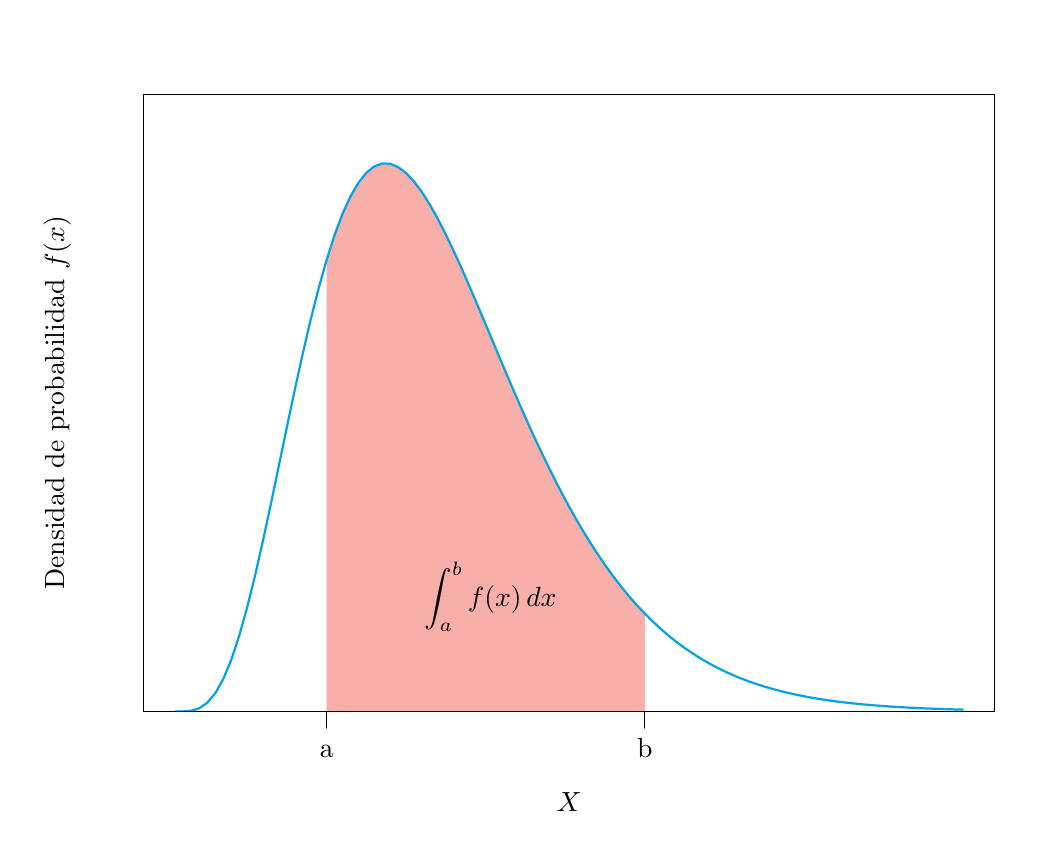
\begin{tikzpicture}[x=1pt,y=1pt]
\definecolor{fillColor}{RGB}{255,255,255}
\path[use as bounding box,fill=fillColor,fill opacity=0.00] (0,0) rectangle (361.35,289.08);
\begin{scope}
\path[clip] (  0.00,  0.00) rectangle (361.35,289.08);
\definecolor{drawColor}{RGB}{0,0,0}

\node[text=drawColor,anchor=base,inner sep=0pt, outer sep=0pt, scale=  1.00] at (195.67,  6.00) {$X$};

\node[text=drawColor,rotate= 90.00,anchor=base,inner sep=0pt, outer sep=0pt, scale=  1.00] at ( 13.20,153.54) {Densidad de probabilidad $f(x)$};
\end{scope}
\begin{scope}
\path[clip] (  0.00,  0.00) rectangle (361.35,289.08);
\definecolor{drawColor}{RGB}{0,0,0}

\path[draw=drawColor,line width= 0.4pt,line join=round,line cap=round] (108.00, 42.00) -- (222.98, 42.00);

\path[draw=drawColor,line width= 0.4pt,line join=round,line cap=round] (108.00, 42.00) -- (108.00, 36.00);

\path[draw=drawColor,line width= 0.4pt,line join=round,line cap=round] (222.98, 42.00) -- (222.98, 36.00);

\node[text=drawColor,anchor=base,inner sep=0pt, outer sep=0pt, scale=  1.00] at (108.00, 25.20) {a};

\node[text=drawColor,anchor=base,inner sep=0pt, outer sep=0pt, scale=  1.00] at (222.98, 25.20) {b};
\end{scope}
\begin{scope}
\path[clip] ( 42.00, 42.00) rectangle (349.35,265.08);
\definecolor{fillColor}{RGB}{238,50,36}

\path[fill=fillColor,fill opacity=0.39] (108.00, 42.00) --
	(108.00,205.09) --
	(110.87,214.08) --
	(113.75,221.76) --
	(116.62,228.08) --
	(119.50,233.03) --
	(122.37,236.65) --
	(125.25,238.95) --
	(128.12,240.01) --
	(131.00,239.90) --
	(133.87,238.71) --
	(136.75,236.53) --
	(139.62,233.46) --
	(142.50,229.60) --
	(145.37,225.05) --
	(148.24,219.92) --
	(151.12,214.30) --
	(153.99,208.28) --
	(156.87,201.95) --
	(159.74,195.38) --
	(162.62,188.66) --
	(165.49,181.84) --
	(168.37,174.99) --
	(171.24,168.15) --
	(174.12,161.39) --
	(176.99,154.73) --
	(179.86,148.21) --
	(182.74,141.86) --
	(185.61,135.71) --
	(188.49,129.77) --
	(191.36,124.06) --
	(194.24,118.58) --
	(197.11,113.35) --
	(199.99,108.38) --
	(202.86,103.65) --
	(205.74, 99.18) --
	(208.61, 94.96) --
	(211.49, 90.98) --
	(214.36, 87.24) --
	(217.23, 83.73) --
	(220.11, 80.44) --
	(222.98, 77.38) --
	(222.98, 42.00) --
	cycle;
\definecolor{drawColor}{RGB}{5,161,230}

\path[draw=drawColor,line width= 0.8pt,line join=round,line cap=round] ( 53.38, 42.00) --
	( 56.26, 42.02) --
	( 59.13, 42.26) --
	( 62.01, 43.14) --
	( 64.88, 45.11) --
	( 67.76, 48.52) --
	( 70.63, 53.63) --
	( 73.51, 60.51) --
	( 76.38, 69.14) --
	( 79.25, 79.36) --
	( 82.13, 90.94) --
	( 85.00,103.57) --
	( 87.88,116.95) --
	( 90.75,130.71) --
	( 93.63,144.55) --
	( 96.50,158.14) --
	( 99.38,171.21) --
	(102.25,183.52) --
	(105.13,194.86) --
	(108.00,205.09) --
	(110.87,214.08) --
	(113.75,221.76) --
	(116.62,228.08) --
	(119.50,233.03) --
	(122.37,236.65) --
	(125.25,238.95) --
	(128.12,240.01) --
	(131.00,239.90) --
	(133.87,238.71) --
	(136.75,236.53) --
	(139.62,233.46) --
	(142.50,229.60) --
	(145.37,225.05) --
	(148.24,219.92) --
	(151.12,214.30) --
	(153.99,208.28) --
	(156.87,201.95) --
	(159.74,195.38) --
	(162.62,188.66) --
	(165.49,181.84) --
	(168.37,174.99) --
	(171.24,168.15) --
	(174.12,161.39) --
	(176.99,154.73) --
	(179.86,148.21) --
	(182.74,141.86) --
	(185.61,135.71) --
	(188.49,129.77) --
	(191.36,124.06) --
	(194.24,118.58) --
	(197.11,113.35) --
	(199.99,108.38) --
	(202.86,103.65) --
	(205.74, 99.18) --
	(208.61, 94.96) --
	(211.49, 90.98) --
	(214.36, 87.24) --
	(217.23, 83.73) --
	(220.11, 80.44) --
	(222.98, 77.38) --
	(225.86, 74.52) --
	(228.73, 71.86) --
	(231.61, 69.38) --
	(234.48, 67.09) --
	(237.36, 64.96) --
	(240.23, 63.00) --
	(243.11, 61.18) --
	(245.98, 59.51) --
	(248.85, 57.96) --
	(251.73, 56.54) --
	(254.60, 55.24) --
	(257.48, 54.04) --
	(260.35, 52.95) --
	(263.23, 51.94) --
	(266.10, 51.02) --
	(268.98, 50.18) --
	(271.85, 49.41) --
	(274.73, 48.71) --
	(277.60, 48.07) --
	(280.48, 47.49) --
	(283.35, 46.96) --
	(286.22, 46.48) --
	(289.10, 46.05) --
	(291.97, 45.65) --
	(294.85, 45.29) --
	(297.72, 44.97) --
	(300.60, 44.67) --
	(303.47, 44.40) --
	(306.35, 44.16) --
	(309.22, 43.94) --
	(312.10, 43.75) --
	(314.97, 43.57) --
	(317.84, 43.41) --
	(320.72, 43.26) --
	(323.59, 43.13) --
	(326.47, 43.02) --
	(329.34, 42.91) --
	(332.22, 42.82) --
	(335.09, 42.73) --
	(337.97, 42.65);
\definecolor{drawColor}{RGB}{0,0,0}

\node[text=drawColor,anchor=base,inner sep=0pt, outer sep=0pt, scale=  1.00] at (167.22, 80.06) {$\displaystyle \int_a^b f(x)\,dx$};
\end{scope}
\begin{scope}
\path[clip] (  0.00,  0.00) rectangle (361.35,289.08);
\definecolor{drawColor}{RGB}{0,0,0}

\path[draw=drawColor,line width= 0.4pt,line join=round,line cap=round] ( 42.00, 42.00) --
	(349.35, 42.00) --
	(349.35,265.08) --
	( 42.00,265.08) --
	( 42.00, 42.00);
\end{scope}
\end{tikzpicture}
}}
	\mode<presentation>{\resizebox{0.7\textwidth}{!}{% Created by tikzDevice version 0.9 on 2016-04-28 16:54:50
% !TEX encoding = UTF-8 Unicode
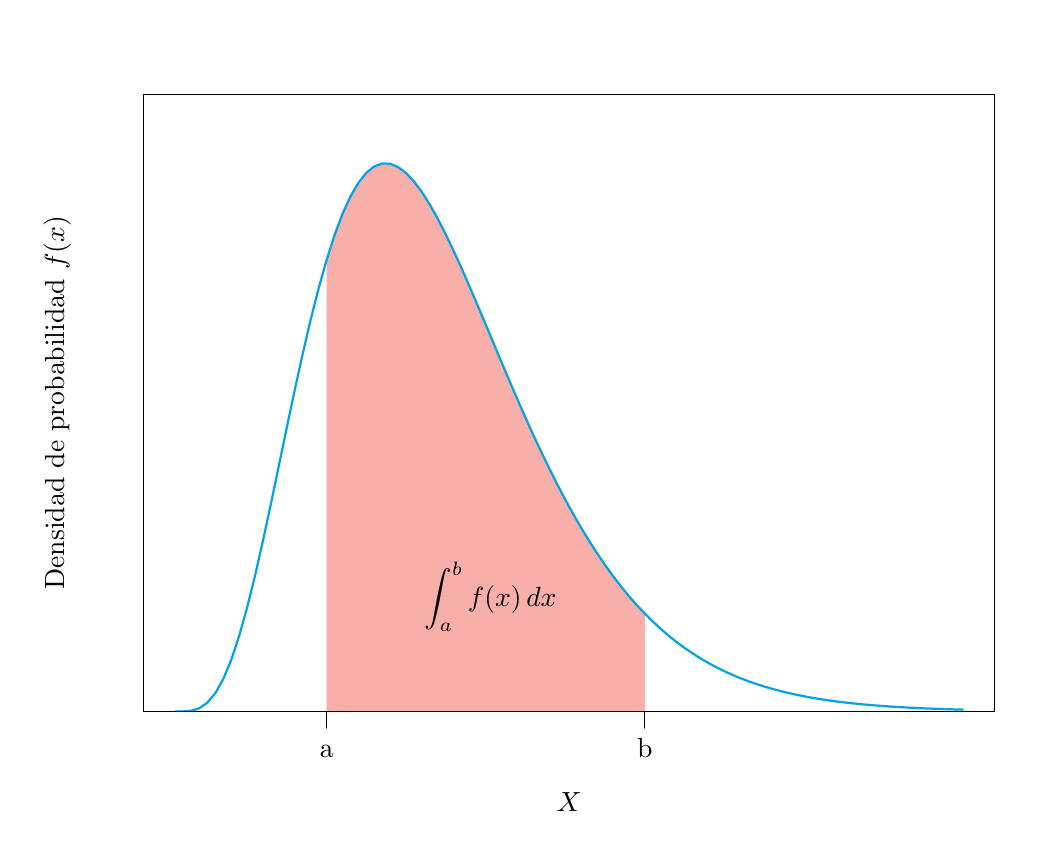
\begin{tikzpicture}[x=1pt,y=1pt]
\definecolor{fillColor}{RGB}{255,255,255}
\path[use as bounding box,fill=fillColor,fill opacity=0.00] (0,0) rectangle (361.35,289.08);
\begin{scope}
\path[clip] (  0.00,  0.00) rectangle (361.35,289.08);
\definecolor{drawColor}{RGB}{0,0,0}

\node[text=drawColor,anchor=base,inner sep=0pt, outer sep=0pt, scale=  1.00] at (195.67,  6.00) {$X$};

\node[text=drawColor,rotate= 90.00,anchor=base,inner sep=0pt, outer sep=0pt, scale=  1.00] at ( 13.20,153.54) {Densidad de probabilidad $f(x)$};
\end{scope}
\begin{scope}
\path[clip] (  0.00,  0.00) rectangle (361.35,289.08);
\definecolor{drawColor}{RGB}{0,0,0}

\path[draw=drawColor,line width= 0.4pt,line join=round,line cap=round] (108.00, 42.00) -- (222.98, 42.00);

\path[draw=drawColor,line width= 0.4pt,line join=round,line cap=round] (108.00, 42.00) -- (108.00, 36.00);

\path[draw=drawColor,line width= 0.4pt,line join=round,line cap=round] (222.98, 42.00) -- (222.98, 36.00);

\node[text=drawColor,anchor=base,inner sep=0pt, outer sep=0pt, scale=  1.00] at (108.00, 25.20) {a};

\node[text=drawColor,anchor=base,inner sep=0pt, outer sep=0pt, scale=  1.00] at (222.98, 25.20) {b};
\end{scope}
\begin{scope}
\path[clip] ( 42.00, 42.00) rectangle (349.35,265.08);
\definecolor{fillColor}{RGB}{238,50,36}

\path[fill=fillColor,fill opacity=0.39] (108.00, 42.00) --
	(108.00,205.09) --
	(110.87,214.08) --
	(113.75,221.76) --
	(116.62,228.08) --
	(119.50,233.03) --
	(122.37,236.65) --
	(125.25,238.95) --
	(128.12,240.01) --
	(131.00,239.90) --
	(133.87,238.71) --
	(136.75,236.53) --
	(139.62,233.46) --
	(142.50,229.60) --
	(145.37,225.05) --
	(148.24,219.92) --
	(151.12,214.30) --
	(153.99,208.28) --
	(156.87,201.95) --
	(159.74,195.38) --
	(162.62,188.66) --
	(165.49,181.84) --
	(168.37,174.99) --
	(171.24,168.15) --
	(174.12,161.39) --
	(176.99,154.73) --
	(179.86,148.21) --
	(182.74,141.86) --
	(185.61,135.71) --
	(188.49,129.77) --
	(191.36,124.06) --
	(194.24,118.58) --
	(197.11,113.35) --
	(199.99,108.38) --
	(202.86,103.65) --
	(205.74, 99.18) --
	(208.61, 94.96) --
	(211.49, 90.98) --
	(214.36, 87.24) --
	(217.23, 83.73) --
	(220.11, 80.44) --
	(222.98, 77.38) --
	(222.98, 42.00) --
	cycle;
\definecolor{drawColor}{RGB}{5,161,230}

\path[draw=drawColor,line width= 0.8pt,line join=round,line cap=round] ( 53.38, 42.00) --
	( 56.26, 42.02) --
	( 59.13, 42.26) --
	( 62.01, 43.14) --
	( 64.88, 45.11) --
	( 67.76, 48.52) --
	( 70.63, 53.63) --
	( 73.51, 60.51) --
	( 76.38, 69.14) --
	( 79.25, 79.36) --
	( 82.13, 90.94) --
	( 85.00,103.57) --
	( 87.88,116.95) --
	( 90.75,130.71) --
	( 93.63,144.55) --
	( 96.50,158.14) --
	( 99.38,171.21) --
	(102.25,183.52) --
	(105.13,194.86) --
	(108.00,205.09) --
	(110.87,214.08) --
	(113.75,221.76) --
	(116.62,228.08) --
	(119.50,233.03) --
	(122.37,236.65) --
	(125.25,238.95) --
	(128.12,240.01) --
	(131.00,239.90) --
	(133.87,238.71) --
	(136.75,236.53) --
	(139.62,233.46) --
	(142.50,229.60) --
	(145.37,225.05) --
	(148.24,219.92) --
	(151.12,214.30) --
	(153.99,208.28) --
	(156.87,201.95) --
	(159.74,195.38) --
	(162.62,188.66) --
	(165.49,181.84) --
	(168.37,174.99) --
	(171.24,168.15) --
	(174.12,161.39) --
	(176.99,154.73) --
	(179.86,148.21) --
	(182.74,141.86) --
	(185.61,135.71) --
	(188.49,129.77) --
	(191.36,124.06) --
	(194.24,118.58) --
	(197.11,113.35) --
	(199.99,108.38) --
	(202.86,103.65) --
	(205.74, 99.18) --
	(208.61, 94.96) --
	(211.49, 90.98) --
	(214.36, 87.24) --
	(217.23, 83.73) --
	(220.11, 80.44) --
	(222.98, 77.38) --
	(225.86, 74.52) --
	(228.73, 71.86) --
	(231.61, 69.38) --
	(234.48, 67.09) --
	(237.36, 64.96) --
	(240.23, 63.00) --
	(243.11, 61.18) --
	(245.98, 59.51) --
	(248.85, 57.96) --
	(251.73, 56.54) --
	(254.60, 55.24) --
	(257.48, 54.04) --
	(260.35, 52.95) --
	(263.23, 51.94) --
	(266.10, 51.02) --
	(268.98, 50.18) --
	(271.85, 49.41) --
	(274.73, 48.71) --
	(277.60, 48.07) --
	(280.48, 47.49) --
	(283.35, 46.96) --
	(286.22, 46.48) --
	(289.10, 46.05) --
	(291.97, 45.65) --
	(294.85, 45.29) --
	(297.72, 44.97) --
	(300.60, 44.67) --
	(303.47, 44.40) --
	(306.35, 44.16) --
	(309.22, 43.94) --
	(312.10, 43.75) --
	(314.97, 43.57) --
	(317.84, 43.41) --
	(320.72, 43.26) --
	(323.59, 43.13) --
	(326.47, 43.02) --
	(329.34, 42.91) --
	(332.22, 42.82) --
	(335.09, 42.73) --
	(337.97, 42.65);
\definecolor{drawColor}{RGB}{0,0,0}

\node[text=drawColor,anchor=base,inner sep=0pt, outer sep=0pt, scale=  1.00] at (167.22, 80.06) {$\displaystyle \int_a^b f(x)\,dx$};
\end{scope}
\begin{scope}
\path[clip] (  0.00,  0.00) rectangle (361.35,289.08);
\definecolor{drawColor}{RGB}{0,0,0}

\path[draw=drawColor,line width= 0.4pt,line join=round,line cap=round] ( 42.00, 42.00) --
	(349.35, 42.00) --
	(349.35,265.08) --
	( 42.00,265.08) --
	( 42.00, 42.00);
\end{scope}
\end{tikzpicture}
}}
	$\displaystyle P(a\leq X\leq b) = \int_a^b f(x)\, dx = F(b)-F(a)$
\end{center}

\note{
Como ya hemos dicho, la función de densidad nos permite calcular la probabilidad un intervalo $[a,b]$ como el área acumulada por debajo de
la función en dicho intervalo.

Para ello tenemos dos posibilidades, a partir de la función de la función de densidad, calculando la integral definidad de esta entre $a$ y
$b$ o, a partir de la función de distribución, midiendo el área acumulada por debajo de $b$ y restandole el área acumulada por debajo de $a$
para quedarnos precisamente con el área que hay entre $a$ y $b$. Como es más fácil hacer restas que calcular integrales, trabajaremos la
mayoría de las veces con funciones de distribución. 
}
\end{frame}


%---------------------------------------------------------------------slide----
\begin{frame}
\frametitle{Cálculo de probabilidades como áreas}
\framesubtitle{Ejemplo}
Dada la siguiente función:
\[
f(x) = 
\begin{cases}
0 & \mbox{si $x<0$}\\
e^{-x} & \mbox{si $x\geq 0$},
\end{cases}
\]
veamos que se trata de una función de densidad. 

Como es evidente que la función es no negativa, solo que da por comprobar que el área por debajo de ella es 1.
\begin{align*}
\int_{-\infty}^\infty f(x)\;dx &= \int_{-\infty}^0 f(x)\;dx +\int_0^\infty f(x)\;dx = \int_{-\infty}^0 0\;dx +\int_0^\infty e^{-x}\;dx =\\
&= \left[-e^{-x}\right]_0^{\infty} = -e^{-\infty}+e^0 = 1.
\end{align*}
Calculemos la probabilidad de que la variable tome un valor entre 0 y 2.
\begin{align*}
P(0\leq X\leq 2) &= \int_0^2 f(x)\;dx = \int_0^2 e^{-x}\;dx = \left[-e^{-x}\right]_0^2 = -e^{-2}+e^0 = 0.8646. 
\end{align*}

\note{
Veamos un ejemplo.
}
\end{frame}


%---------------------------------------------------------------------slide----
\begin{frame}
\frametitle{Estadísticos poblacionales}
El cálculo de los estadísticos poblacionales es similar al caso discreto, pero utilizando la función de densidad en lugar de la función de
probabilidad, y extendiendo la suma discreta a la integral en todo el rango de la variable.

Los más importantes son:
\begin{itemize}
\item \structure{Media o esperanza matemática}:
\[
\mu = E(X) = \int_{-\infty}^\infty x f(x)\; dx
\]
\item \structure{Varianza}:
\[
\sigma^2 = Var(X) = \int_{-\infty}^\infty x^2f(x)\; dx -\mu^2
\]
\item \structure{Desviación típica}:
\[
\sigma = +\sqrt{\sigma^2}
\] 
\end{itemize}

\note{
El cálculo de los estadísticos poblacionales es similar al caso discreto, pero utilizando la función de densidad, en lugar de la función de
probabilidad, y extendiendo la suma discreta a la integral en todo el recorrido de la variable.

Así la media se define como 
\begin{itemize}
\item \structure{Media o esperanza matemática}:
\[
\mu = E(X) = \int_{-\infty}^\infty x f(x)\; dx
\]
\item \structure{Varianza}:
\[
\sigma^2 = Var(X) = \int_{-\infty}^\infty x^2f(x)\; dx -\mu^2
\]
\item \structure{Desviación típica}:
\[
\sigma = +\sqrt{\sigma^2}
\] 
\end{itemize}
}
\end{frame}


%---------------------------------------------------------------------slide----
\begin{frame}
\frametitle{Cálculo de los estadísticos poblacionales}
\framesubtitle{Ejemplo}
Sea $X$ una variable aleatoria con la siguiente función de densidad:
\[
f(x) = 
\begin{cases}
0 & \mbox{si $x<0$}\\
e^{-x} & \mbox{si $x\geq 0$}
\end{cases}
\]

Su media es
\begin{align*}
\mu &= \int_{-\infty}^\infty xf(x)\;dx = \int_{-\infty}^0 xf(x)\;dx +\int_0^\infty xf(x)\;dx = \int_{-\infty}^0 0\;dx +\int_0^\infty xe^{-x}\;dx =\\
&= \left[-e^{-x}(1+x)\right]_0^{\infty} = 1.
\end{align*}
y su varianza vale
\begin{align*}
\sigma^2 &= \int_{-\infty}^\infty x^2f(x)\;dx -\mu^2 = \int_{-\infty}^0 x^2f(x)\;dx +\int_0^\infty x^2f(x)\;dx -\mu^2 = \\
&= \int_{-\infty}^0 0\;dx +\int_0^\infty x^2e^{-x}\;dx -\mu^2= \left[-e^{-x}(x^2+2x+2)\right]_0^{\infty} - 1^2= 2e^0-1 = 1.
\end{align*}

\note{
Siguiendo con el ejemplo anterior, la media vale:
}
\end{frame}



%---------------------------------------------------------------------slide----
\begin{frame}
\frametitle{Modelos de distribución continuos}
Existen varios modelos de distribución de probabilidad que aparecen bastante a menudo en la naturaleza y también como consecuencia de los
procesos de muestreo aleatorio simple.
Los más importantes son:

\begin{itemize}
\item Distribución Uniforme continua.
\item Distribución Normal.
\item Distribución T de Student.
\item Distribución Chi-cuadrado.
\item Distribución F de Fisher-Snedecor.
\end{itemize}

\note{
Existen varios modelos de distribución de probabilidad que aparecen bastante a menudo en la naturaleza y también como consecuencia de los
procesos de muestreo aleatorio simple.

A continuación veremos los más importantes:
\begin{itemize}
\item Distribución Uniforme continua.
\item Distribución Normal.
\item Distribución T de Student.
\item Distribución Chi-cuadrado.
\item Distribución F de Fisher-Snedecor.
\end{itemize}
}
\end{frame}


\subsection{Distribución Uniforme continua}

%---------------------------------------------------------------------slide----
\begin{frame}
\frametitle{Distribución Uniforme continua $U(a,b)$}
Cuando todos los valores de una variable continua son equiprobables, se dice que la variable sigue un \emph{modelo de distribución uniforme
continuo}.

\begin{definicion}[Distribución Uniforme continua $U(a,b)$]
Una variable aleatoria continua $X$, sigue un modelo de distribución de probabilidad \emph{uniforme}, y se nota $X\sim U(a,b)$, si su rango es $\mbox{Ran}(X) = [a,b]$ y su función de densidad es 
\[
f(x)= \frac{1}{b-a}\quad \forall x\in [a,b]
\]
\end{definicion}

Obsérvese que $a$ y $b$ son el mínimo y el máximo del rango respectivamente, y que la función de densidad es constante.

Su media y varianza valen
\[
\mu = \frac{a+b}{2}\qquad \sigma^2=\frac{(b-a)^2}{12}.
\]

\note{
Al igual que para variables discretas, cuando todos los valores de una variable continua son equiprobables, se dice que la variable sigue
un \emph{modelo de distribución uniforme continuo}.

Si el recorrido de la variable es el intervalo $[a,b]$ entonces se dice que sigue un modelo de distribución \emph{uniforme} $U(a,b)$, y se
cumple que su función de densidad es constante y vale:
\[
f(x)= \frac{1}{b-a}\quad \forall x\in [a,b]
\]

Además, su media vale
\[
\mu = \frac{a+b}{2}.
\]
y su varianza
\[
\sigma^2=\frac{(b-a)^2}{12}.
\]
}
\end{frame}


%---------------------------------------------------------------------slide----
\begin{frame}
\frametitle{Función de densidad de la Uniforme continua $U(a,b)$}
\framesubtitle{Ejemplo}
La generación aleatoria de un número real entre 0 y 1 sigue un modelo de distribución uniforme continuo $U(0,1)$. 
\begin{center}
	\tikzsetnextfilename{variables_aleatorias_continuas/funcion_densidad_uniforme}
	\mode<article>{\resizebox{0.6\textwidth}{!}{% Created by tikzDevice version 0.9 on 2016-04-28 17:31:47
% !TEX encoding = UTF-8 Unicode
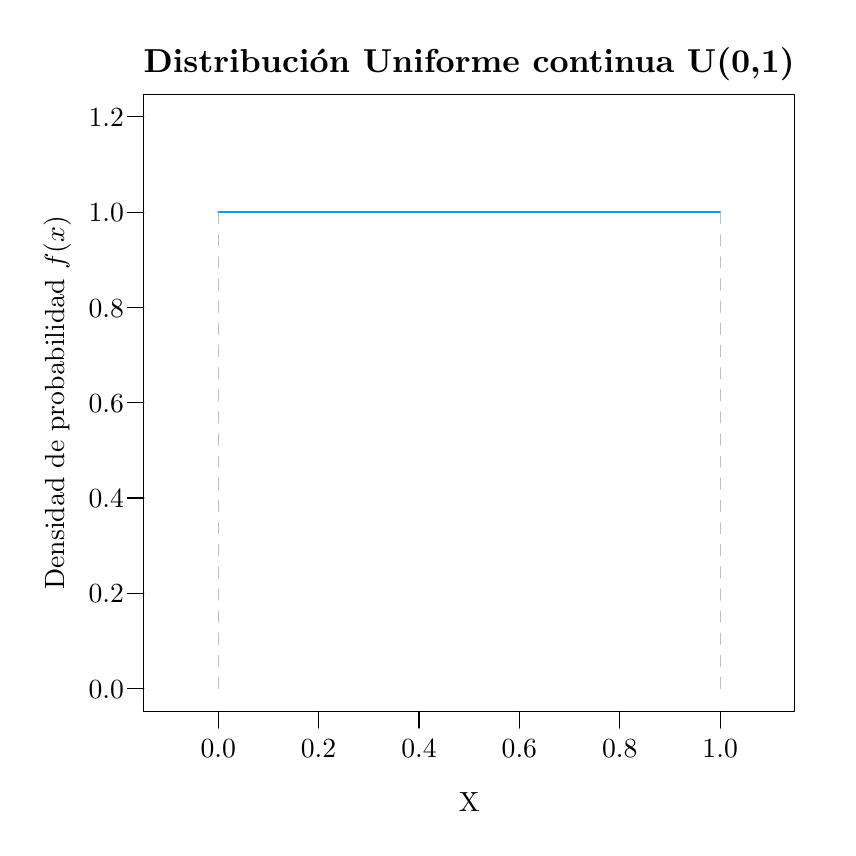
\begin{tikzpicture}[x=1pt,y=1pt]
\definecolor{fillColor}{RGB}{255,255,255}
\path[use as bounding box,fill=fillColor,fill opacity=0.00] (0,0) rectangle (289.08,289.08);
\begin{scope}
\path[clip] ( 42.00, 42.00) rectangle (277.08,265.08);
\definecolor{drawColor}{RGB}{5,161,230}

\path[draw=drawColor,line width= 0.8pt,line join=round,line cap=round] ( 68.85,222.39) --
	( 89.00,222.39) --
	(109.15,222.39) --
	(129.31,222.39) --
	(149.46,222.39) --
	(169.62,222.39) --
	(189.77,222.39) --
	(209.93,222.39) --
	(230.08,222.39) --
	(250.23,222.39);
\end{scope}
\begin{scope}
\path[clip] (  0.00,  0.00) rectangle (289.08,289.08);
\definecolor{drawColor}{RGB}{0,0,0}

\path[draw=drawColor,line width= 0.4pt,line join=round,line cap=round] ( 68.85, 42.00) -- (250.23, 42.00);

\path[draw=drawColor,line width= 0.4pt,line join=round,line cap=round] ( 68.85, 42.00) -- ( 68.85, 36.00);

\path[draw=drawColor,line width= 0.4pt,line join=round,line cap=round] (105.12, 42.00) -- (105.12, 36.00);

\path[draw=drawColor,line width= 0.4pt,line join=round,line cap=round] (141.40, 42.00) -- (141.40, 36.00);

\path[draw=drawColor,line width= 0.4pt,line join=round,line cap=round] (177.68, 42.00) -- (177.68, 36.00);

\path[draw=drawColor,line width= 0.4pt,line join=round,line cap=round] (213.96, 42.00) -- (213.96, 36.00);

\path[draw=drawColor,line width= 0.4pt,line join=round,line cap=round] (250.23, 42.00) -- (250.23, 36.00);

\node[text=drawColor,anchor=base,inner sep=0pt, outer sep=0pt, scale=  1.00] at ( 68.85, 25.20) {0.0};

\node[text=drawColor,anchor=base,inner sep=0pt, outer sep=0pt, scale=  1.00] at (105.12, 25.20) {0.2};

\node[text=drawColor,anchor=base,inner sep=0pt, outer sep=0pt, scale=  1.00] at (141.40, 25.20) {0.4};

\node[text=drawColor,anchor=base,inner sep=0pt, outer sep=0pt, scale=  1.00] at (177.68, 25.20) {0.6};

\node[text=drawColor,anchor=base,inner sep=0pt, outer sep=0pt, scale=  1.00] at (213.96, 25.20) {0.8};

\node[text=drawColor,anchor=base,inner sep=0pt, outer sep=0pt, scale=  1.00] at (250.23, 25.20) {1.0};

\path[draw=drawColor,line width= 0.4pt,line join=round,line cap=round] ( 42.00, 50.26) -- ( 42.00,256.82);

\path[draw=drawColor,line width= 0.4pt,line join=round,line cap=round] ( 42.00, 50.26) -- ( 36.00, 50.26);

\path[draw=drawColor,line width= 0.4pt,line join=round,line cap=round] ( 42.00, 84.69) -- ( 36.00, 84.69);

\path[draw=drawColor,line width= 0.4pt,line join=round,line cap=round] ( 42.00,119.11) -- ( 36.00,119.11);

\path[draw=drawColor,line width= 0.4pt,line join=round,line cap=round] ( 42.00,153.54) -- ( 36.00,153.54);

\path[draw=drawColor,line width= 0.4pt,line join=round,line cap=round] ( 42.00,187.97) -- ( 36.00,187.97);

\path[draw=drawColor,line width= 0.4pt,line join=round,line cap=round] ( 42.00,222.39) -- ( 36.00,222.39);

\path[draw=drawColor,line width= 0.4pt,line join=round,line cap=round] ( 42.00,256.82) -- ( 36.00,256.82);

\node[text=drawColor,anchor=base east,inner sep=0pt, outer sep=0pt, scale=  1.00] at ( 34.80, 46.82) {0.0};

\node[text=drawColor,anchor=base east,inner sep=0pt, outer sep=0pt, scale=  1.00] at ( 34.80, 81.24) {0.2};

\node[text=drawColor,anchor=base east,inner sep=0pt, outer sep=0pt, scale=  1.00] at ( 34.80,115.67) {0.4};

\node[text=drawColor,anchor=base east,inner sep=0pt, outer sep=0pt, scale=  1.00] at ( 34.80,150.10) {0.6};

\node[text=drawColor,anchor=base east,inner sep=0pt, outer sep=0pt, scale=  1.00] at ( 34.80,184.52) {0.8};

\node[text=drawColor,anchor=base east,inner sep=0pt, outer sep=0pt, scale=  1.00] at ( 34.80,218.95) {1.0};

\node[text=drawColor,anchor=base east,inner sep=0pt, outer sep=0pt, scale=  1.00] at ( 34.80,253.37) {1.2};

\path[draw=drawColor,line width= 0.4pt,line join=round,line cap=round] ( 42.00, 42.00) --
	(277.08, 42.00) --
	(277.08,265.08) --
	( 42.00,265.08) --
	( 42.00, 42.00);
\end{scope}
\begin{scope}
\path[clip] (  0.00,  0.00) rectangle (289.08,289.08);
\definecolor{drawColor}{RGB}{0,0,0}

\node[text=drawColor,anchor=base,inner sep=0pt, outer sep=0pt, scale=  1.20] at (159.54,272.89) {\bfseries Distribución Uniforme continua U(0,1)};

\node[text=drawColor,anchor=base,inner sep=0pt, outer sep=0pt, scale=  1.00] at (159.54,  6.00) {X};

\node[text=drawColor,rotate= 90.00,anchor=base,inner sep=0pt, outer sep=0pt, scale=  1.00] at ( 13.20,153.54) {Densidad de probabilidad $f(x)$};
\end{scope}
\begin{scope}
\path[clip] ( 42.00, 42.00) rectangle (277.08,265.08);
\definecolor{drawColor}{RGB}{190,190,190}

\path[draw=drawColor,line width= 0.4pt,dash pattern=on 4pt off 4pt ,line join=round,line cap=round] ( 68.85, 50.26) -- ( 68.85,222.39);

\path[draw=drawColor,line width= 0.4pt,dash pattern=on 4pt off 4pt ,line join=round,line cap=round] (250.23, 50.26) -- (250.23,222.39);
\end{scope}
\end{tikzpicture}
}}
	\mode<presentation>{\resizebox{0.6\textwidth}{!}{% Created by tikzDevice version 0.9 on 2016-04-28 17:31:47
% !TEX encoding = UTF-8 Unicode
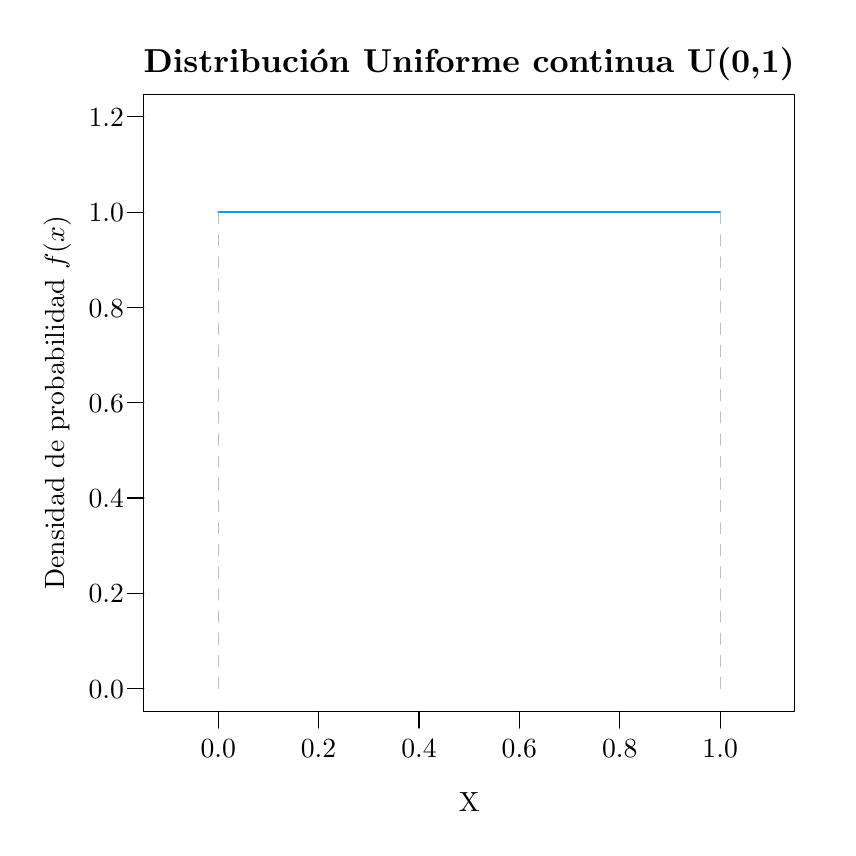
\begin{tikzpicture}[x=1pt,y=1pt]
\definecolor{fillColor}{RGB}{255,255,255}
\path[use as bounding box,fill=fillColor,fill opacity=0.00] (0,0) rectangle (289.08,289.08);
\begin{scope}
\path[clip] ( 42.00, 42.00) rectangle (277.08,265.08);
\definecolor{drawColor}{RGB}{5,161,230}

\path[draw=drawColor,line width= 0.8pt,line join=round,line cap=round] ( 68.85,222.39) --
	( 89.00,222.39) --
	(109.15,222.39) --
	(129.31,222.39) --
	(149.46,222.39) --
	(169.62,222.39) --
	(189.77,222.39) --
	(209.93,222.39) --
	(230.08,222.39) --
	(250.23,222.39);
\end{scope}
\begin{scope}
\path[clip] (  0.00,  0.00) rectangle (289.08,289.08);
\definecolor{drawColor}{RGB}{0,0,0}

\path[draw=drawColor,line width= 0.4pt,line join=round,line cap=round] ( 68.85, 42.00) -- (250.23, 42.00);

\path[draw=drawColor,line width= 0.4pt,line join=round,line cap=round] ( 68.85, 42.00) -- ( 68.85, 36.00);

\path[draw=drawColor,line width= 0.4pt,line join=round,line cap=round] (105.12, 42.00) -- (105.12, 36.00);

\path[draw=drawColor,line width= 0.4pt,line join=round,line cap=round] (141.40, 42.00) -- (141.40, 36.00);

\path[draw=drawColor,line width= 0.4pt,line join=round,line cap=round] (177.68, 42.00) -- (177.68, 36.00);

\path[draw=drawColor,line width= 0.4pt,line join=round,line cap=round] (213.96, 42.00) -- (213.96, 36.00);

\path[draw=drawColor,line width= 0.4pt,line join=round,line cap=round] (250.23, 42.00) -- (250.23, 36.00);

\node[text=drawColor,anchor=base,inner sep=0pt, outer sep=0pt, scale=  1.00] at ( 68.85, 25.20) {0.0};

\node[text=drawColor,anchor=base,inner sep=0pt, outer sep=0pt, scale=  1.00] at (105.12, 25.20) {0.2};

\node[text=drawColor,anchor=base,inner sep=0pt, outer sep=0pt, scale=  1.00] at (141.40, 25.20) {0.4};

\node[text=drawColor,anchor=base,inner sep=0pt, outer sep=0pt, scale=  1.00] at (177.68, 25.20) {0.6};

\node[text=drawColor,anchor=base,inner sep=0pt, outer sep=0pt, scale=  1.00] at (213.96, 25.20) {0.8};

\node[text=drawColor,anchor=base,inner sep=0pt, outer sep=0pt, scale=  1.00] at (250.23, 25.20) {1.0};

\path[draw=drawColor,line width= 0.4pt,line join=round,line cap=round] ( 42.00, 50.26) -- ( 42.00,256.82);

\path[draw=drawColor,line width= 0.4pt,line join=round,line cap=round] ( 42.00, 50.26) -- ( 36.00, 50.26);

\path[draw=drawColor,line width= 0.4pt,line join=round,line cap=round] ( 42.00, 84.69) -- ( 36.00, 84.69);

\path[draw=drawColor,line width= 0.4pt,line join=round,line cap=round] ( 42.00,119.11) -- ( 36.00,119.11);

\path[draw=drawColor,line width= 0.4pt,line join=round,line cap=round] ( 42.00,153.54) -- ( 36.00,153.54);

\path[draw=drawColor,line width= 0.4pt,line join=round,line cap=round] ( 42.00,187.97) -- ( 36.00,187.97);

\path[draw=drawColor,line width= 0.4pt,line join=round,line cap=round] ( 42.00,222.39) -- ( 36.00,222.39);

\path[draw=drawColor,line width= 0.4pt,line join=round,line cap=round] ( 42.00,256.82) -- ( 36.00,256.82);

\node[text=drawColor,anchor=base east,inner sep=0pt, outer sep=0pt, scale=  1.00] at ( 34.80, 46.82) {0.0};

\node[text=drawColor,anchor=base east,inner sep=0pt, outer sep=0pt, scale=  1.00] at ( 34.80, 81.24) {0.2};

\node[text=drawColor,anchor=base east,inner sep=0pt, outer sep=0pt, scale=  1.00] at ( 34.80,115.67) {0.4};

\node[text=drawColor,anchor=base east,inner sep=0pt, outer sep=0pt, scale=  1.00] at ( 34.80,150.10) {0.6};

\node[text=drawColor,anchor=base east,inner sep=0pt, outer sep=0pt, scale=  1.00] at ( 34.80,184.52) {0.8};

\node[text=drawColor,anchor=base east,inner sep=0pt, outer sep=0pt, scale=  1.00] at ( 34.80,218.95) {1.0};

\node[text=drawColor,anchor=base east,inner sep=0pt, outer sep=0pt, scale=  1.00] at ( 34.80,253.37) {1.2};

\path[draw=drawColor,line width= 0.4pt,line join=round,line cap=round] ( 42.00, 42.00) --
	(277.08, 42.00) --
	(277.08,265.08) --
	( 42.00,265.08) --
	( 42.00, 42.00);
\end{scope}
\begin{scope}
\path[clip] (  0.00,  0.00) rectangle (289.08,289.08);
\definecolor{drawColor}{RGB}{0,0,0}

\node[text=drawColor,anchor=base,inner sep=0pt, outer sep=0pt, scale=  1.20] at (159.54,272.89) {\bfseries Distribución Uniforme continua U(0,1)};

\node[text=drawColor,anchor=base,inner sep=0pt, outer sep=0pt, scale=  1.00] at (159.54,  6.00) {X};

\node[text=drawColor,rotate= 90.00,anchor=base,inner sep=0pt, outer sep=0pt, scale=  1.00] at ( 13.20,153.54) {Densidad de probabilidad $f(x)$};
\end{scope}
\begin{scope}
\path[clip] ( 42.00, 42.00) rectangle (277.08,265.08);
\definecolor{drawColor}{RGB}{190,190,190}

\path[draw=drawColor,line width= 0.4pt,dash pattern=on 4pt off 4pt ,line join=round,line cap=round] ( 68.85, 50.26) -- ( 68.85,222.39);

\path[draw=drawColor,line width= 0.4pt,dash pattern=on 4pt off 4pt ,line join=round,line cap=round] (250.23, 50.26) -- (250.23,222.39);
\end{scope}
\end{tikzpicture}
}}
\end{center}

\note{
Un ejemplo de variable aleatoria uniforme continua sería la que mide el resultado de generar aleatoriamente un número entre 0 y 1. Esta
variable seguiría un modelo de distribución uniforme continuo $U(0,1)$, y la gráfica de su función de densidad es esta. Como se ve, la
función es constante y vale 1, ya que debe cumplirse, al ser función de densidad, que el área total por debajo de ella debe ser 1, y como en
realidad se trata del área de un rectángulo de base 1, pues la altura debe ser también 1.
}
\end{frame}


%---------------------------------------------------------------------slide----
\begin{frame}
\frametitle{Función de distribución de la Uniforme continua $U(a,b)$}
\framesubtitle{Ejemplo}
Como la función de densidad es constante, la función de distribución presenta un crecimiento lineal.
\begin{center}
	\tikzsetnextfilename{variables_aleatorias_continuas/funcion_distribucion_uniforme}
	\mode<article>{\resizebox{0.6\textwidth}{!}{% Created by tikzDevice version 0.9 on 2016-04-28 17:47:04
% !TEX encoding = UTF-8 Unicode
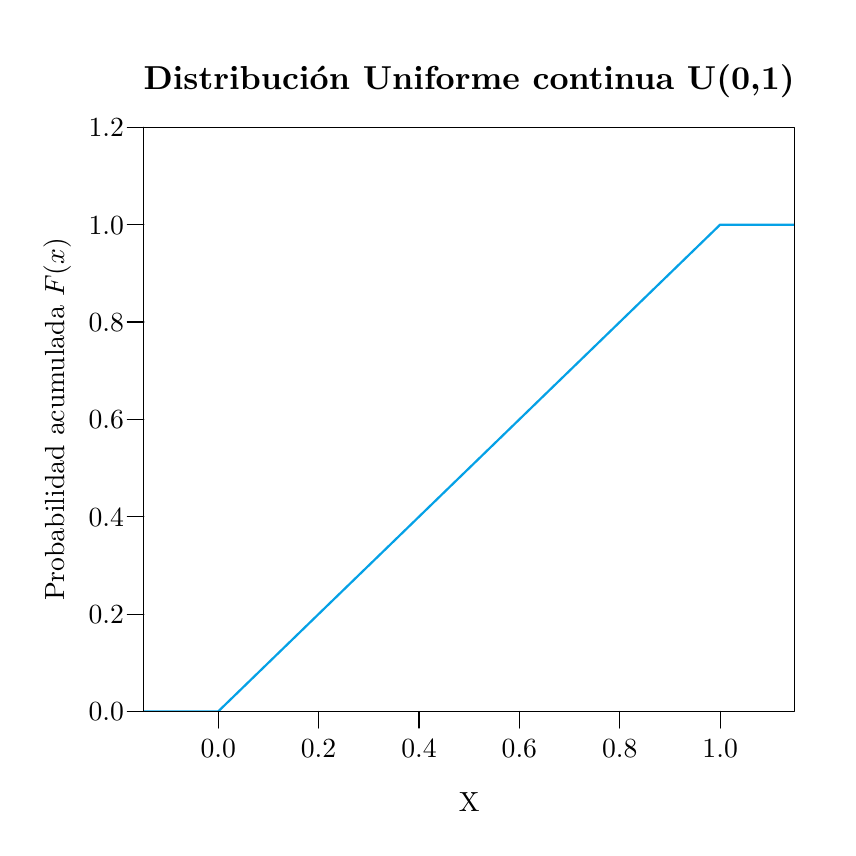
\begin{tikzpicture}[x=1pt,y=1pt]
\definecolor{fillColor}{RGB}{255,255,255}
\path[use as bounding box,fill=fillColor,fill opacity=0.00] (0,0) rectangle (289.08,289.08);
\begin{scope}
\path[clip] ( 42.00, 42.00) rectangle (277.08,253.08);
\definecolor{drawColor}{RGB}{5,161,230}

\path[draw=drawColor,line width= 0.8pt,line join=round,line cap=round] ( 32.57, 42.00) --
	( 68.85, 42.00) --
	( 89.00, 61.54) --
	(109.15, 81.09) --
	(129.31,100.63) --
	(149.46,120.18) --
	(169.62,139.72) --
	(189.77,159.27) --
	(209.93,178.81) --
	(230.08,198.36) --
	(250.23,217.90) --
	(286.51,217.90);
\end{scope}
\begin{scope}
\path[clip] (  0.00,  0.00) rectangle (289.08,289.08);
\definecolor{drawColor}{RGB}{0,0,0}

\path[draw=drawColor,line width= 0.4pt,line join=round,line cap=round] ( 68.85, 42.00) -- (250.23, 42.00);

\path[draw=drawColor,line width= 0.4pt,line join=round,line cap=round] ( 68.85, 42.00) -- ( 68.85, 36.00);

\path[draw=drawColor,line width= 0.4pt,line join=round,line cap=round] (105.12, 42.00) -- (105.12, 36.00);

\path[draw=drawColor,line width= 0.4pt,line join=round,line cap=round] (141.40, 42.00) -- (141.40, 36.00);

\path[draw=drawColor,line width= 0.4pt,line join=round,line cap=round] (177.68, 42.00) -- (177.68, 36.00);

\path[draw=drawColor,line width= 0.4pt,line join=round,line cap=round] (213.96, 42.00) -- (213.96, 36.00);

\path[draw=drawColor,line width= 0.4pt,line join=round,line cap=round] (250.23, 42.00) -- (250.23, 36.00);

\node[text=drawColor,anchor=base,inner sep=0pt, outer sep=0pt, scale=  1.00] at ( 68.85, 25.20) {0.0};

\node[text=drawColor,anchor=base,inner sep=0pt, outer sep=0pt, scale=  1.00] at (105.12, 25.20) {0.2};

\node[text=drawColor,anchor=base,inner sep=0pt, outer sep=0pt, scale=  1.00] at (141.40, 25.20) {0.4};

\node[text=drawColor,anchor=base,inner sep=0pt, outer sep=0pt, scale=  1.00] at (177.68, 25.20) {0.6};

\node[text=drawColor,anchor=base,inner sep=0pt, outer sep=0pt, scale=  1.00] at (213.96, 25.20) {0.8};

\node[text=drawColor,anchor=base,inner sep=0pt, outer sep=0pt, scale=  1.00] at (250.23, 25.20) {1.0};

\path[draw=drawColor,line width= 0.4pt,line join=round,line cap=round] ( 42.00, 42.00) -- ( 42.00,253.08);

\path[draw=drawColor,line width= 0.4pt,line join=round,line cap=round] ( 42.00, 42.00) -- ( 36.00, 42.00);

\path[draw=drawColor,line width= 0.4pt,line join=round,line cap=round] ( 42.00, 77.18) -- ( 36.00, 77.18);

\path[draw=drawColor,line width= 0.4pt,line join=round,line cap=round] ( 42.00,112.36) -- ( 36.00,112.36);

\path[draw=drawColor,line width= 0.4pt,line join=round,line cap=round] ( 42.00,147.54) -- ( 36.00,147.54);

\path[draw=drawColor,line width= 0.4pt,line join=round,line cap=round] ( 42.00,182.72) -- ( 36.00,182.72);

\path[draw=drawColor,line width= 0.4pt,line join=round,line cap=round] ( 42.00,217.90) -- ( 36.00,217.90);

\path[draw=drawColor,line width= 0.4pt,line join=round,line cap=round] ( 42.00,253.08) -- ( 36.00,253.08);

\node[text=drawColor,anchor=base east,inner sep=0pt, outer sep=0pt, scale=  1.00] at ( 34.80, 38.56) {0.0};

\node[text=drawColor,anchor=base east,inner sep=0pt, outer sep=0pt, scale=  1.00] at ( 34.80, 73.74) {0.2};

\node[text=drawColor,anchor=base east,inner sep=0pt, outer sep=0pt, scale=  1.00] at ( 34.80,108.92) {0.4};

\node[text=drawColor,anchor=base east,inner sep=0pt, outer sep=0pt, scale=  1.00] at ( 34.80,144.10) {0.6};

\node[text=drawColor,anchor=base east,inner sep=0pt, outer sep=0pt, scale=  1.00] at ( 34.80,179.28) {0.8};

\node[text=drawColor,anchor=base east,inner sep=0pt, outer sep=0pt, scale=  1.00] at ( 34.80,214.46) {1.0};

\node[text=drawColor,anchor=base east,inner sep=0pt, outer sep=0pt, scale=  1.00] at ( 34.80,249.64) {1.2};

\path[draw=drawColor,line width= 0.4pt,line join=round,line cap=round] ( 42.00, 42.00) --
	(277.08, 42.00) --
	(277.08,253.08) --
	( 42.00,253.08) --
	( 42.00, 42.00);
\end{scope}
\begin{scope}
\path[clip] (  0.00,  0.00) rectangle (289.08,289.08);
\definecolor{drawColor}{RGB}{0,0,0}

\node[text=drawColor,anchor=base,inner sep=0pt, outer sep=0pt, scale=  1.20] at (159.54,266.89) {\bfseries Distribución Uniforme continua U(0,1)};

\node[text=drawColor,anchor=base,inner sep=0pt, outer sep=0pt, scale=  1.00] at (159.54,  6.00) {X};

\node[text=drawColor,rotate= 90.00,anchor=base,inner sep=0pt, outer sep=0pt, scale=  1.00] at ( 13.20,147.54) {Probabilidad acumulada $F(x)$};
\end{scope}
\end{tikzpicture}
}}
	\mode<presentation>{\resizebox{0.6\textwidth}{!}{% Created by tikzDevice version 0.9 on 2016-04-28 17:47:04
% !TEX encoding = UTF-8 Unicode
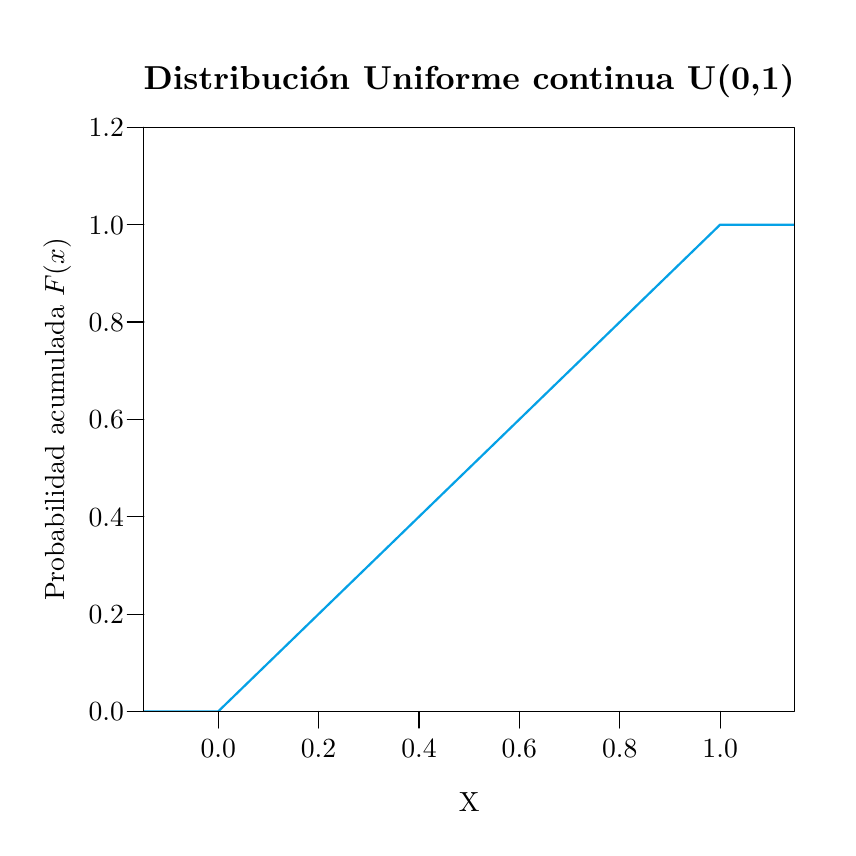
\begin{tikzpicture}[x=1pt,y=1pt]
\definecolor{fillColor}{RGB}{255,255,255}
\path[use as bounding box,fill=fillColor,fill opacity=0.00] (0,0) rectangle (289.08,289.08);
\begin{scope}
\path[clip] ( 42.00, 42.00) rectangle (277.08,253.08);
\definecolor{drawColor}{RGB}{5,161,230}

\path[draw=drawColor,line width= 0.8pt,line join=round,line cap=round] ( 32.57, 42.00) --
	( 68.85, 42.00) --
	( 89.00, 61.54) --
	(109.15, 81.09) --
	(129.31,100.63) --
	(149.46,120.18) --
	(169.62,139.72) --
	(189.77,159.27) --
	(209.93,178.81) --
	(230.08,198.36) --
	(250.23,217.90) --
	(286.51,217.90);
\end{scope}
\begin{scope}
\path[clip] (  0.00,  0.00) rectangle (289.08,289.08);
\definecolor{drawColor}{RGB}{0,0,0}

\path[draw=drawColor,line width= 0.4pt,line join=round,line cap=round] ( 68.85, 42.00) -- (250.23, 42.00);

\path[draw=drawColor,line width= 0.4pt,line join=round,line cap=round] ( 68.85, 42.00) -- ( 68.85, 36.00);

\path[draw=drawColor,line width= 0.4pt,line join=round,line cap=round] (105.12, 42.00) -- (105.12, 36.00);

\path[draw=drawColor,line width= 0.4pt,line join=round,line cap=round] (141.40, 42.00) -- (141.40, 36.00);

\path[draw=drawColor,line width= 0.4pt,line join=round,line cap=round] (177.68, 42.00) -- (177.68, 36.00);

\path[draw=drawColor,line width= 0.4pt,line join=round,line cap=round] (213.96, 42.00) -- (213.96, 36.00);

\path[draw=drawColor,line width= 0.4pt,line join=round,line cap=round] (250.23, 42.00) -- (250.23, 36.00);

\node[text=drawColor,anchor=base,inner sep=0pt, outer sep=0pt, scale=  1.00] at ( 68.85, 25.20) {0.0};

\node[text=drawColor,anchor=base,inner sep=0pt, outer sep=0pt, scale=  1.00] at (105.12, 25.20) {0.2};

\node[text=drawColor,anchor=base,inner sep=0pt, outer sep=0pt, scale=  1.00] at (141.40, 25.20) {0.4};

\node[text=drawColor,anchor=base,inner sep=0pt, outer sep=0pt, scale=  1.00] at (177.68, 25.20) {0.6};

\node[text=drawColor,anchor=base,inner sep=0pt, outer sep=0pt, scale=  1.00] at (213.96, 25.20) {0.8};

\node[text=drawColor,anchor=base,inner sep=0pt, outer sep=0pt, scale=  1.00] at (250.23, 25.20) {1.0};

\path[draw=drawColor,line width= 0.4pt,line join=round,line cap=round] ( 42.00, 42.00) -- ( 42.00,253.08);

\path[draw=drawColor,line width= 0.4pt,line join=round,line cap=round] ( 42.00, 42.00) -- ( 36.00, 42.00);

\path[draw=drawColor,line width= 0.4pt,line join=round,line cap=round] ( 42.00, 77.18) -- ( 36.00, 77.18);

\path[draw=drawColor,line width= 0.4pt,line join=round,line cap=round] ( 42.00,112.36) -- ( 36.00,112.36);

\path[draw=drawColor,line width= 0.4pt,line join=round,line cap=round] ( 42.00,147.54) -- ( 36.00,147.54);

\path[draw=drawColor,line width= 0.4pt,line join=round,line cap=round] ( 42.00,182.72) -- ( 36.00,182.72);

\path[draw=drawColor,line width= 0.4pt,line join=round,line cap=round] ( 42.00,217.90) -- ( 36.00,217.90);

\path[draw=drawColor,line width= 0.4pt,line join=round,line cap=round] ( 42.00,253.08) -- ( 36.00,253.08);

\node[text=drawColor,anchor=base east,inner sep=0pt, outer sep=0pt, scale=  1.00] at ( 34.80, 38.56) {0.0};

\node[text=drawColor,anchor=base east,inner sep=0pt, outer sep=0pt, scale=  1.00] at ( 34.80, 73.74) {0.2};

\node[text=drawColor,anchor=base east,inner sep=0pt, outer sep=0pt, scale=  1.00] at ( 34.80,108.92) {0.4};

\node[text=drawColor,anchor=base east,inner sep=0pt, outer sep=0pt, scale=  1.00] at ( 34.80,144.10) {0.6};

\node[text=drawColor,anchor=base east,inner sep=0pt, outer sep=0pt, scale=  1.00] at ( 34.80,179.28) {0.8};

\node[text=drawColor,anchor=base east,inner sep=0pt, outer sep=0pt, scale=  1.00] at ( 34.80,214.46) {1.0};

\node[text=drawColor,anchor=base east,inner sep=0pt, outer sep=0pt, scale=  1.00] at ( 34.80,249.64) {1.2};

\path[draw=drawColor,line width= 0.4pt,line join=round,line cap=round] ( 42.00, 42.00) --
	(277.08, 42.00) --
	(277.08,253.08) --
	( 42.00,253.08) --
	( 42.00, 42.00);
\end{scope}
\begin{scope}
\path[clip] (  0.00,  0.00) rectangle (289.08,289.08);
\definecolor{drawColor}{RGB}{0,0,0}

\node[text=drawColor,anchor=base,inner sep=0pt, outer sep=0pt, scale=  1.20] at (159.54,266.89) {\bfseries Distribución Uniforme continua U(0,1)};

\node[text=drawColor,anchor=base,inner sep=0pt, outer sep=0pt, scale=  1.00] at (159.54,  6.00) {X};

\node[text=drawColor,rotate= 90.00,anchor=base,inner sep=0pt, outer sep=0pt, scale=  1.00] at ( 13.20,147.54) {Probabilidad acumulada $F(x)$};
\end{scope}
\end{tikzpicture}
}}
\end{center}

\note{
En esta otra gráfica tenemos la función de distribución $U(0,1)$.
Como la función de densidad es constante, la función de distribución presenta un crecimiento lineal. Obsérvese que, como para cualquier
función de distribución, la probabilidad acumulada al comienzo del recorrido es 0, y al final, vale 1, que es la probabilidad total. 
}
\end{frame}


% ---------------------------------------------------------------------slide----
\begin{frame}
\frametitle{Cálculo de probabilidades con una Uniforme continua}
\framesubtitle{Ejemplo de espera de un autobús}
Un autobús pasa por una parada cada 15 minutos. 
Si una persona puede llegar a la parada en cualquier instante, \emph{¿cuál es
la probabilidad de que espere entre 5 y 10 minutos?}
\begin{columns}
\begin{column}{0.52\textwidth}
En este caso, la variable $X$ que mide el tiempo de espera sigue un modelo de distribución uniforme continua $U(0,15)$ ya que cualquier valor entre los 0 y los 15 minutos es equipobrable.

Así pues, la probabilidad de esperar entre 5 y 10 minutos es
\begin{align*}
P(5\leq X\leq 10) &= \int_{5}^{10} \frac{1}{15}\;dx = \left[\frac{x}{15}\right]_5^{10} = \\
&= \frac{10}{15}-\frac{5}{15} =\frac{1}{3}.
\end{align*}
\end{column}
\begin{column}{0.43\textwidth}
\begin{center}
	\tikzsetnextfilename{variables_aleatorias_continuas/calculo_probabilidades_uniforme}
	\mode<article>{\resizebox{0.6\textwidth}{!}{%% Input file name: calculo_probabilidades_uniforme.fig
%% FIG version: 3.2
%% Orientation: Landscape
%% Justification: Flush Left
%% Units: Inches
%% Paper size: A4
%% Magnification: 100.0
%% Resolution: 1200ppi
%% Include the following in the preamble:
%% \usepackage{textcomp}
%% End

\begin{pspicture}(6.68cm,3.48cm)(16.66cm,13.45cm)
\psset{unit=0.8cm}
%%
%% Depth: 2147483647
%%
\newgray{mycolor0}{0.74}\definecolor{mycolor0}{gray}{0.74}
\newrgbcolor{mycolor1}{1.00 0.50 0.31}\definecolor{mycolor1}{rgb}{1.00,0.50,0.31}
%%
%% Depth: 100
%%
\psset{linestyle=solid,linewidth=0.03175,linecolor=black,fillstyle=none}
\psline(10.90,13.59)(13.82,13.59)(16.73,13.59)(19.64,13.59)
\psset{fillstyle=solid,fillcolor=mycolor1}
\psline(13.82,6.80)(13.82,13.59)(16.73,13.59)(16.73,6.80)
\psset{fillstyle=none}
\psline(10.90,6.47)(19.64,6.47)
\psline(10.90,6.47)(10.90,6.26)
\psline(13.82,6.47)(13.82,6.26)
\psline(16.73,6.47)(16.73,6.26)
\psline(19.64,6.47)(19.64,6.26)
\rput(10.90,5.71){0}
\rput(13.82,5.71){5}
\rput(16.73,5.71){10}
\rput(19.64,5.71){15}
\psline(10.23,6.80)(10.23,14.95)
\psline(10.23,6.80)(10.02,6.80)
\psline(10.23,8.84)(10.02,8.84)
\psline(10.23,10.88)(10.02,10.88)
\psline(10.23,12.91)(10.02,12.91)
\psline(10.23,14.95)(10.02,14.95)
\rput{90}(9.73,6.80){0.00}
\rput{90}(9.73,8.84){0.02}
\rput{90}(9.73,10.88){0.04}
\rput{90}(9.73,12.91){0.06}
\rput{90}(9.73,14.95){0.08}
\psline(10.23,6.47)(20.31,6.47)(20.31,15.28)(10.23,15.28)(10.23,6.47)
\rput(15.27,15.99){Distribución Uniforme $U(0,15)$}
\rput(15.27,4.86){$X$}
\rput[l]{90}(8.86,9.54){Densidad $f(x)$}
\psset{linecolor=mycolor0}
\psline(10.23,6.80)(20.31,6.80)
\rput(15.27,10.78){$P(5\leq X\leq 10)=$}
\rput(15.27,9.76){$\int_5^{10}\frac{1}{15}\;dx$}
\psset{linestyle=dashed}
\psline(10.90,6.80)(10.90,13.59)
\psline(19.64,6.80)(19.64,13.59)
\end{pspicture}
%% End
}}
	\mode<presentation>{\resizebox{1\textwidth}{!}{%% Input file name: calculo_probabilidades_uniforme.fig
%% FIG version: 3.2
%% Orientation: Landscape
%% Justification: Flush Left
%% Units: Inches
%% Paper size: A4
%% Magnification: 100.0
%% Resolution: 1200ppi
%% Include the following in the preamble:
%% \usepackage{textcomp}
%% End

\begin{pspicture}(6.68cm,3.48cm)(16.66cm,13.45cm)
\psset{unit=0.8cm}
%%
%% Depth: 2147483647
%%
\newgray{mycolor0}{0.74}\definecolor{mycolor0}{gray}{0.74}
\newrgbcolor{mycolor1}{1.00 0.50 0.31}\definecolor{mycolor1}{rgb}{1.00,0.50,0.31}
%%
%% Depth: 100
%%
\psset{linestyle=solid,linewidth=0.03175,linecolor=black,fillstyle=none}
\psline(10.90,13.59)(13.82,13.59)(16.73,13.59)(19.64,13.59)
\psset{fillstyle=solid,fillcolor=mycolor1}
\psline(13.82,6.80)(13.82,13.59)(16.73,13.59)(16.73,6.80)
\psset{fillstyle=none}
\psline(10.90,6.47)(19.64,6.47)
\psline(10.90,6.47)(10.90,6.26)
\psline(13.82,6.47)(13.82,6.26)
\psline(16.73,6.47)(16.73,6.26)
\psline(19.64,6.47)(19.64,6.26)
\rput(10.90,5.71){0}
\rput(13.82,5.71){5}
\rput(16.73,5.71){10}
\rput(19.64,5.71){15}
\psline(10.23,6.80)(10.23,14.95)
\psline(10.23,6.80)(10.02,6.80)
\psline(10.23,8.84)(10.02,8.84)
\psline(10.23,10.88)(10.02,10.88)
\psline(10.23,12.91)(10.02,12.91)
\psline(10.23,14.95)(10.02,14.95)
\rput{90}(9.73,6.80){0.00}
\rput{90}(9.73,8.84){0.02}
\rput{90}(9.73,10.88){0.04}
\rput{90}(9.73,12.91){0.06}
\rput{90}(9.73,14.95){0.08}
\psline(10.23,6.47)(20.31,6.47)(20.31,15.28)(10.23,15.28)(10.23,6.47)
\rput(15.27,15.99){Distribución Uniforme $U(0,15)$}
\rput(15.27,4.86){$X$}
\rput[l]{90}(8.86,9.54){Densidad $f(x)$}
\psset{linecolor=mycolor0}
\psline(10.23,6.80)(20.31,6.80)
\rput(15.27,10.78){$P(5\leq X\leq 10)=$}
\rput(15.27,9.76){$\int_5^{10}\frac{1}{15}\;dx$}
\psset{linestyle=dashed}
\psline(10.90,6.80)(10.90,13.59)
\psline(19.64,6.80)(19.64,13.59)
\end{pspicture}
%% End
}}
\end{center}
\end{column}
\end{columns}
Además, el tiempo medio de espera será $\mu=\frac{0+15}{2}=7.5$ minutos.

\note{
Como ejemplo, supóngase que un autobús pasa por una parada cada 15 minutos. Si una persona puede llegar a la parada en cualquier instante,
\emph{¿cuál es la probabilidad de que espere entre 5 y 10 minutos?}

Está claro que lo mínimo que puede esperar una persona es 0 minutos, si llega justo cuando está el autobús, y lo máximo es 15 minutos, si
llega justo cuando el autobús se marcha. Como además puede llegar en cualquier instante con equiprobabiliadad, la variable $X$ que mide el
tiempo de espera sigue un modelo de distribución uniforme continua $U(0,15)$.

Así pues, la probabilidad que nos piden es
\begin{align*}
P(5\leq X\leq 10) &= \int_{5}^{10} \frac{1}{15}\;dx = \left[\frac{x}{15}\right]_5^{10} = \\
&= \frac{10}{15}-\frac{5}{15} =\frac{1}{3}.
\end{align*}

Aunque también podría calcularse fácilmente a partir de la gráfica de la función de densidad que es constante y vale $1/15$, midiendo el
área que queda por debajo de esta función entre 5 y 10. Como se tráta del área de un rectánculo, basta multiplicar la base, que es 5, por la
altura que es $1/15$ y de nuevo se obtiene $1/3$.
}
\end{frame}


\subsection{Distribución Normal}

%---------------------------------------------------------------------slide----
\begin{frame}
\frametitle{Distribución de probabilidad Normal $N(\mu,\sigma)$}
El modelo de distribución normal es, sin duda, el modelo de distribución continuo más importante, ya que es el que más a menudo se presenta
en la naturaleza.

\begin{definicion}[Distribución de probabilidad Normal $N(\mu,\sigma)$]
Una variable aleatoria continua $X$ sigue un modelo de distribución \emph{normal} de parámetros $\mu$ y $\sigma$, y se nota $X\sim N(\mu,\sigma)$, si su rango es $\mathbb{R}$ y su función de densidad vale
\[
f(x)= \frac{1}{\sigma\sqrt{2\pi}}e^{-\frac{(x-\mu)^2}{2\sigma^2}}.
\]
\end{definicion}

Los dos parámetros $\mu$ y $\sigma$ son la media y la desviación típica de la población respectivamente.

\note{
El modelo de distribución normal es, sin duda, el modelo de distribución continuo más importante, ya que es el que más a menudo se presenta
en la naturaleza, sobre todo en variables continuas biológicas.

\begin{definicion}[Distribución Normal]
Una variable aleatoria continua $X$ sigue un modelo de distribución \emph{normal} $N(\mu,\sigma)$ si su recorrido es $\mathbb{R}$ y su función de densidad vale
\[
f(x)= \frac{1}{\sigma\sqrt{2\pi}}e^{-\frac{(x-\mu)^2}{2\sigma^2}}.
\]
\end{definicion}

La distribución normal depende de dos parámetros $\mu$ y $\sigma$ que son, precisamente, su media y desviación típica.
}
\end{frame}


%---------------------------------------------------------------------slide----
\begin{frame}
\frametitle{Función de densidad de la Normal}
La gráfica de la función de densidad de la distribución normal tiene forma de una especie de campana, conocida como \emph{campana de Gauss}
(en honor a su descubridor).
\begin{center}
	\tikzsetnextfilename{variables_aleatorias_continuas/funcion_densidad_normal}
	\mode<article>{\resizebox{0.6\textwidth}{!}{% Created by tikzDevice version 0.10.1 on 2016-05-08 18:26:45
% !TEX encoding = UTF-8 Unicode
\begin{tikzpicture}[x=1pt,y=1pt]
\definecolor{fillColor}{RGB}{255,255,255}
\path[use as bounding box,fill=fillColor,fill opacity=0.00] (0,0) rectangle (289.08,289.08);
\begin{scope}
\path[clip] ( 42.00, 42.00) rectangle (277.08,253.08);
\definecolor{drawColor}{RGB}{5,161,230}

\path[draw=drawColor,line width= 0.8pt,line join=round,line cap=round] ( 50.71, 42.81) --
	( 52.36, 42.95) --
	( 54.00, 43.12) --
	( 55.65, 43.31) --
	( 57.30, 43.53) --
	( 58.95, 43.79) --
	( 60.60, 44.08) --
	( 62.25, 44.41) --
	( 63.90, 44.79) --
	( 65.55, 45.22) --
	( 67.20, 45.71) --
	( 68.85, 46.27) --
	( 70.49, 46.89) --
	( 72.14, 47.59) --
	( 73.79, 48.37) --
	( 75.44, 49.25) --
	( 77.09, 50.22) --
	( 78.74, 51.31) --
	( 80.39, 52.50) --
	( 82.04, 53.83) --
	( 83.69, 55.29) --
	( 85.34, 56.89) --
	( 86.98, 58.64) --
	( 88.63, 60.55) --
	( 90.28, 62.63) --
	( 91.93, 64.89) --
	( 93.58, 67.33) --
	( 95.23, 69.95) --
	( 96.88, 72.78) --
	( 98.53, 75.80) --
	(100.18, 79.03) --
	(101.83, 82.47) --
	(103.47, 86.12) --
	(105.12, 89.97) --
	(106.77, 94.03) --
	(108.42, 98.29) --
	(110.07,102.75) --
	(111.72,107.40) --
	(113.37,112.23) --
	(115.02,117.23) --
	(116.67,122.38) --
	(118.32,127.67) --
	(119.96,133.09) --
	(121.61,138.60) --
	(123.26,144.19) --
	(124.91,149.83) --
	(126.56,155.50) --
	(128.21,161.17) --
	(129.86,166.81) --
	(131.51,172.39) --
	(133.16,177.88) --
	(134.81,183.25) --
	(136.45,188.47) --
	(138.10,193.50) --
	(139.75,198.30) --
	(141.40,202.86) --
	(143.05,207.14) --
	(144.70,211.11) --
	(146.35,214.74) --
	(148.00,218.01) --
	(149.65,220.90) --
	(151.30,223.37) --
	(152.94,225.43) --
	(154.59,227.04) --
	(156.24,228.20) --
	(157.89,228.90) --
	(159.54,229.13) --
	(161.19,228.90) --
	(162.84,228.20) --
	(164.49,227.04) --
	(166.14,225.43) --
	(167.78,223.37) --
	(169.43,220.90) --
	(171.08,218.01) --
	(172.73,214.74) --
	(174.38,211.11) --
	(176.03,207.14) --
	(177.68,202.86) --
	(179.33,198.30) --
	(180.98,193.50) --
	(182.63,188.47) --
	(184.27,183.25) --
	(185.92,177.88) --
	(187.57,172.39) --
	(189.22,166.81) --
	(190.87,161.17) --
	(192.52,155.50) --
	(194.17,149.83) --
	(195.82,144.19) --
	(197.47,138.60) --
	(199.12,133.09) --
	(200.76,127.67) --
	(202.41,122.38) --
	(204.06,117.23) --
	(205.71,112.23) --
	(207.36,107.40) --
	(209.01,102.75) --
	(210.66, 98.29) --
	(212.31, 94.03) --
	(213.96, 89.97) --
	(215.61, 86.12) --
	(217.25, 82.47) --
	(218.90, 79.03) --
	(220.55, 75.80) --
	(222.20, 72.78) --
	(223.85, 69.95) --
	(225.50, 67.33) --
	(227.15, 64.89) --
	(228.80, 62.63) --
	(230.45, 60.55) --
	(232.10, 58.64) --
	(233.74, 56.89) --
	(235.39, 55.29) --
	(237.04, 53.83) --
	(238.69, 52.50) --
	(240.34, 51.31) --
	(241.99, 50.22) --
	(243.64, 49.25) --
	(245.29, 48.37) --
	(246.94, 47.59) --
	(248.59, 46.89) --
	(250.23, 46.27) --
	(251.88, 45.71) --
	(253.53, 45.22) --
	(255.18, 44.79) --
	(256.83, 44.41) --
	(258.48, 44.08) --
	(260.13, 43.79) --
	(261.78, 43.53) --
	(263.43, 43.31) --
	(265.08, 43.12) --
	(266.72, 42.95) --
	(268.37, 42.81);
\end{scope}
\begin{scope}
\path[clip] (  0.00,  0.00) rectangle (289.08,289.08);
\definecolor{drawColor}{RGB}{0,0,0}

\node[text=drawColor,anchor=base,inner sep=0pt, outer sep=0pt, scale=  1.20] at (159.54,266.89) {\bfseries Distribución Normal $N(\mu,\sigma)$};

\node[text=drawColor,anchor=base,inner sep=0pt, outer sep=0pt, scale=  1.00] at (159.54,  6.00) {X};

\node[text=drawColor,rotate= 90.00,anchor=base,inner sep=0pt, outer sep=0pt, scale=  1.00] at ( 13.20,147.54) {Densidad de probabilidad $f(x)$};
\end{scope}
\begin{scope}
\path[clip] (  0.00,  0.00) rectangle (289.08,289.08);
\definecolor{drawColor}{RGB}{0,0,0}

\path[draw=drawColor,line width= 0.4pt,line join=round,line cap=round] (159.54, 42.00) -- (159.54, 42.00);

\path[draw=drawColor,line width= 0.4pt,line join=round,line cap=round] (159.54, 42.00) -- (159.54, 36.00);

\node[text=drawColor,anchor=base,inner sep=0pt, outer sep=0pt, scale=  1.00] at (159.54, 25.20) {$\mu$};

\path[draw=drawColor,line width= 0.4pt,line join=round,line cap=round] ( 42.00, 42.00) --
	(277.08, 42.00) --
	(277.08,253.08) --
	( 42.00,253.08) --
	( 42.00, 42.00);
\end{scope}
\end{tikzpicture}
}}
	\mode<presentation>{\resizebox{0.6\textwidth}{!}{% Created by tikzDevice version 0.10.1 on 2016-05-08 18:26:45
% !TEX encoding = UTF-8 Unicode
\begin{tikzpicture}[x=1pt,y=1pt]
\definecolor{fillColor}{RGB}{255,255,255}
\path[use as bounding box,fill=fillColor,fill opacity=0.00] (0,0) rectangle (289.08,289.08);
\begin{scope}
\path[clip] ( 42.00, 42.00) rectangle (277.08,253.08);
\definecolor{drawColor}{RGB}{5,161,230}

\path[draw=drawColor,line width= 0.8pt,line join=round,line cap=round] ( 50.71, 42.81) --
	( 52.36, 42.95) --
	( 54.00, 43.12) --
	( 55.65, 43.31) --
	( 57.30, 43.53) --
	( 58.95, 43.79) --
	( 60.60, 44.08) --
	( 62.25, 44.41) --
	( 63.90, 44.79) --
	( 65.55, 45.22) --
	( 67.20, 45.71) --
	( 68.85, 46.27) --
	( 70.49, 46.89) --
	( 72.14, 47.59) --
	( 73.79, 48.37) --
	( 75.44, 49.25) --
	( 77.09, 50.22) --
	( 78.74, 51.31) --
	( 80.39, 52.50) --
	( 82.04, 53.83) --
	( 83.69, 55.29) --
	( 85.34, 56.89) --
	( 86.98, 58.64) --
	( 88.63, 60.55) --
	( 90.28, 62.63) --
	( 91.93, 64.89) --
	( 93.58, 67.33) --
	( 95.23, 69.95) --
	( 96.88, 72.78) --
	( 98.53, 75.80) --
	(100.18, 79.03) --
	(101.83, 82.47) --
	(103.47, 86.12) --
	(105.12, 89.97) --
	(106.77, 94.03) --
	(108.42, 98.29) --
	(110.07,102.75) --
	(111.72,107.40) --
	(113.37,112.23) --
	(115.02,117.23) --
	(116.67,122.38) --
	(118.32,127.67) --
	(119.96,133.09) --
	(121.61,138.60) --
	(123.26,144.19) --
	(124.91,149.83) --
	(126.56,155.50) --
	(128.21,161.17) --
	(129.86,166.81) --
	(131.51,172.39) --
	(133.16,177.88) --
	(134.81,183.25) --
	(136.45,188.47) --
	(138.10,193.50) --
	(139.75,198.30) --
	(141.40,202.86) --
	(143.05,207.14) --
	(144.70,211.11) --
	(146.35,214.74) --
	(148.00,218.01) --
	(149.65,220.90) --
	(151.30,223.37) --
	(152.94,225.43) --
	(154.59,227.04) --
	(156.24,228.20) --
	(157.89,228.90) --
	(159.54,229.13) --
	(161.19,228.90) --
	(162.84,228.20) --
	(164.49,227.04) --
	(166.14,225.43) --
	(167.78,223.37) --
	(169.43,220.90) --
	(171.08,218.01) --
	(172.73,214.74) --
	(174.38,211.11) --
	(176.03,207.14) --
	(177.68,202.86) --
	(179.33,198.30) --
	(180.98,193.50) --
	(182.63,188.47) --
	(184.27,183.25) --
	(185.92,177.88) --
	(187.57,172.39) --
	(189.22,166.81) --
	(190.87,161.17) --
	(192.52,155.50) --
	(194.17,149.83) --
	(195.82,144.19) --
	(197.47,138.60) --
	(199.12,133.09) --
	(200.76,127.67) --
	(202.41,122.38) --
	(204.06,117.23) --
	(205.71,112.23) --
	(207.36,107.40) --
	(209.01,102.75) --
	(210.66, 98.29) --
	(212.31, 94.03) --
	(213.96, 89.97) --
	(215.61, 86.12) --
	(217.25, 82.47) --
	(218.90, 79.03) --
	(220.55, 75.80) --
	(222.20, 72.78) --
	(223.85, 69.95) --
	(225.50, 67.33) --
	(227.15, 64.89) --
	(228.80, 62.63) --
	(230.45, 60.55) --
	(232.10, 58.64) --
	(233.74, 56.89) --
	(235.39, 55.29) --
	(237.04, 53.83) --
	(238.69, 52.50) --
	(240.34, 51.31) --
	(241.99, 50.22) --
	(243.64, 49.25) --
	(245.29, 48.37) --
	(246.94, 47.59) --
	(248.59, 46.89) --
	(250.23, 46.27) --
	(251.88, 45.71) --
	(253.53, 45.22) --
	(255.18, 44.79) --
	(256.83, 44.41) --
	(258.48, 44.08) --
	(260.13, 43.79) --
	(261.78, 43.53) --
	(263.43, 43.31) --
	(265.08, 43.12) --
	(266.72, 42.95) --
	(268.37, 42.81);
\end{scope}
\begin{scope}
\path[clip] (  0.00,  0.00) rectangle (289.08,289.08);
\definecolor{drawColor}{RGB}{0,0,0}

\node[text=drawColor,anchor=base,inner sep=0pt, outer sep=0pt, scale=  1.20] at (159.54,266.89) {\bfseries Distribución Normal $N(\mu,\sigma)$};

\node[text=drawColor,anchor=base,inner sep=0pt, outer sep=0pt, scale=  1.00] at (159.54,  6.00) {X};

\node[text=drawColor,rotate= 90.00,anchor=base,inner sep=0pt, outer sep=0pt, scale=  1.00] at ( 13.20,147.54) {Densidad de probabilidad $f(x)$};
\end{scope}
\begin{scope}
\path[clip] (  0.00,  0.00) rectangle (289.08,289.08);
\definecolor{drawColor}{RGB}{0,0,0}

\path[draw=drawColor,line width= 0.4pt,line join=round,line cap=round] (159.54, 42.00) -- (159.54, 42.00);

\path[draw=drawColor,line width= 0.4pt,line join=round,line cap=round] (159.54, 42.00) -- (159.54, 36.00);

\node[text=drawColor,anchor=base,inner sep=0pt, outer sep=0pt, scale=  1.00] at (159.54, 25.20) {$\mu$};

\path[draw=drawColor,line width= 0.4pt,line join=round,line cap=round] ( 42.00, 42.00) --
	(277.08, 42.00) --
	(277.08,253.08) --
	( 42.00,253.08) --
	( 42.00, 42.00);
\end{scope}
\end{tikzpicture}
}}
\end{center}

\note{
La gráfica de la función de densidad de la distribución normal tiene forma de una especie de campana, conocida como \emph{campana de Gauss}
(en honor a su descubridor), y está centrada en la media $\mu$.
}
\end{frame}


%---------------------------------------------------------------------slide----
\begin{frame}
\frametitle{Función de densidad de la Normal}
La forma de la campana de Gauss depende de sus dos parámetros:
\begin{itemize}
\item La media $\mu$ determina dónde está centrada la campana.
\item La desviación típica $\sigma$ determina la anchura de la campana.
\end{itemize} 
\begin{columns}
\begin{column}{0.47\textwidth}
	\mode<presentation>{\resizebox{\textwidth}{!}{% Created by tikzDevice version 0.10.1 on 2016-05-08 18:26:47
% !TEX encoding = UTF-8 Unicode
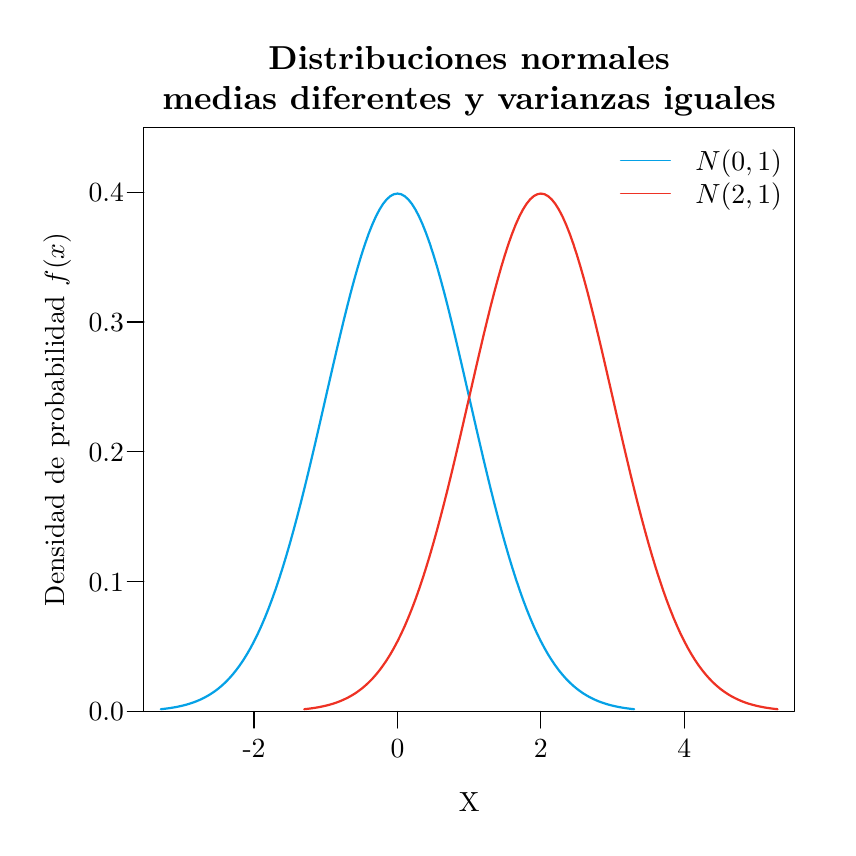
\begin{tikzpicture}[x=1pt,y=1pt]
\definecolor{fillColor}{RGB}{255,255,255}
\path[use as bounding box,fill=fillColor,fill opacity=0.00] (0,0) rectangle (289.08,289.08);
\begin{scope}
\path[clip] ( 42.00, 42.00) rectangle (277.08,253.08);
\definecolor{drawColor}{RGB}{5,161,230}

\path[draw=drawColor,line width= 0.8pt,line join=round,line cap=round] ( 48.12, 42.81) --
	( 49.41, 42.95) --
	( 50.71, 43.12) --
	( 52.00, 43.31) --
	( 53.30, 43.53) --
	( 54.59, 43.79) --
	( 55.89, 44.08) --
	( 57.18, 44.41) --
	( 58.48, 44.79) --
	( 59.78, 45.22) --
	( 61.07, 45.71) --
	( 62.37, 46.27) --
	( 63.66, 46.89) --
	( 64.96, 47.59) --
	( 66.25, 48.37) --
	( 67.55, 49.25) --
	( 68.85, 50.22) --
	( 70.14, 51.31) --
	( 71.44, 52.50) --
	( 72.73, 53.83) --
	( 74.03, 55.29) --
	( 75.32, 56.89) --
	( 76.62, 58.64) --
	( 77.92, 60.55) --
	( 79.21, 62.63) --
	( 80.51, 64.89) --
	( 81.80, 67.33) --
	( 83.10, 69.95) --
	( 84.39, 72.78) --
	( 85.69, 75.80) --
	( 86.98, 79.03) --
	( 88.28, 82.47) --
	( 89.58, 86.12) --
	( 90.87, 89.97) --
	( 92.17, 94.03) --
	( 93.46, 98.29) --
	( 94.76,102.75) --
	( 96.05,107.40) --
	( 97.35,112.23) --
	( 98.65,117.23) --
	( 99.94,122.38) --
	(101.24,127.67) --
	(102.53,133.09) --
	(103.83,138.60) --
	(105.12,144.19) --
	(106.42,149.83) --
	(107.71,155.50) --
	(109.01,161.17) --
	(110.31,166.81) --
	(111.60,172.39) --
	(112.90,177.88) --
	(114.19,183.25) --
	(115.49,188.47) --
	(116.78,193.50) --
	(118.08,198.30) --
	(119.38,202.86) --
	(120.67,207.14) --
	(121.97,211.11) --
	(123.26,214.74) --
	(124.56,218.01) --
	(125.85,220.90) --
	(127.15,223.37) --
	(128.44,225.43) --
	(129.74,227.04) --
	(131.04,228.20) --
	(132.33,228.90) --
	(133.63,229.13) --
	(134.92,228.90) --
	(136.22,228.20) --
	(137.51,227.04) --
	(138.81,225.43) --
	(140.11,223.37) --
	(141.40,220.90) --
	(142.70,218.01) --
	(143.99,214.74) --
	(145.29,211.11) --
	(146.58,207.14) --
	(147.88,202.86) --
	(149.17,198.30) --
	(150.47,193.50) --
	(151.77,188.47) --
	(153.06,183.25) --
	(154.36,177.88) --
	(155.65,172.39) --
	(156.95,166.81) --
	(158.24,161.17) --
	(159.54,155.50) --
	(160.84,149.83) --
	(162.13,144.19) --
	(163.43,138.60) --
	(164.72,133.09) --
	(166.02,127.67) --
	(167.31,122.38) --
	(168.61,117.23) --
	(169.91,112.23) --
	(171.20,107.40) --
	(172.50,102.75) --
	(173.79, 98.29) --
	(175.09, 94.03) --
	(176.38, 89.97) --
	(177.68, 86.12) --
	(178.97, 82.47) --
	(180.27, 79.03) --
	(181.57, 75.80) --
	(182.86, 72.78) --
	(184.16, 69.95) --
	(185.45, 67.33) --
	(186.75, 64.89) --
	(188.04, 62.63) --
	(189.34, 60.55) --
	(190.64, 58.64) --
	(191.93, 56.89) --
	(193.23, 55.29) --
	(194.52, 53.83) --
	(195.82, 52.50) --
	(197.11, 51.31) --
	(198.41, 50.22) --
	(199.70, 49.25) --
	(201.00, 48.37) --
	(202.30, 47.59) --
	(203.59, 46.89) --
	(204.89, 46.27) --
	(206.18, 45.71) --
	(207.48, 45.22) --
	(208.77, 44.79) --
	(210.07, 44.41) --
	(211.37, 44.08) --
	(212.66, 43.79) --
	(213.96, 43.53) --
	(215.25, 43.31) --
	(216.55, 43.12) --
	(217.84, 42.95) --
	(219.14, 42.81);
\end{scope}
\begin{scope}
\path[clip] (  0.00,  0.00) rectangle (289.08,289.08);
\definecolor{drawColor}{RGB}{0,0,0}

\path[draw=drawColor,line width= 0.4pt,line join=round,line cap=round] ( 81.80, 42.00) -- (237.28, 42.00);

\path[draw=drawColor,line width= 0.4pt,line join=round,line cap=round] ( 81.80, 42.00) -- ( 81.80, 36.00);

\path[draw=drawColor,line width= 0.4pt,line join=round,line cap=round] (133.63, 42.00) -- (133.63, 36.00);

\path[draw=drawColor,line width= 0.4pt,line join=round,line cap=round] (185.45, 42.00) -- (185.45, 36.00);

\path[draw=drawColor,line width= 0.4pt,line join=round,line cap=round] (237.28, 42.00) -- (237.28, 36.00);

\node[text=drawColor,anchor=base,inner sep=0pt, outer sep=0pt, scale=  1.00] at ( 81.80, 25.20) {-2};

\node[text=drawColor,anchor=base,inner sep=0pt, outer sep=0pt, scale=  1.00] at (133.63, 25.20) {0};

\node[text=drawColor,anchor=base,inner sep=0pt, outer sep=0pt, scale=  1.00] at (185.45, 25.20) {2};

\node[text=drawColor,anchor=base,inner sep=0pt, outer sep=0pt, scale=  1.00] at (237.28, 25.20) {4};

\path[draw=drawColor,line width= 0.4pt,line join=round,line cap=round] ( 42.00, 42.00) -- ( 42.00,229.63);

\path[draw=drawColor,line width= 0.4pt,line join=round,line cap=round] ( 42.00, 42.00) -- ( 36.00, 42.00);

\path[draw=drawColor,line width= 0.4pt,line join=round,line cap=round] ( 42.00, 88.91) -- ( 36.00, 88.91);

\path[draw=drawColor,line width= 0.4pt,line join=round,line cap=round] ( 42.00,135.81) -- ( 36.00,135.81);

\path[draw=drawColor,line width= 0.4pt,line join=round,line cap=round] ( 42.00,182.72) -- ( 36.00,182.72);

\path[draw=drawColor,line width= 0.4pt,line join=round,line cap=round] ( 42.00,229.63) -- ( 36.00,229.63);

\node[text=drawColor,anchor=base east,inner sep=0pt, outer sep=0pt, scale=  1.00] at ( 34.80, 38.56) {0.0};

\node[text=drawColor,anchor=base east,inner sep=0pt, outer sep=0pt, scale=  1.00] at ( 34.80, 85.46) {0.1};

\node[text=drawColor,anchor=base east,inner sep=0pt, outer sep=0pt, scale=  1.00] at ( 34.80,132.37) {0.2};

\node[text=drawColor,anchor=base east,inner sep=0pt, outer sep=0pt, scale=  1.00] at ( 34.80,179.28) {0.3};

\node[text=drawColor,anchor=base east,inner sep=0pt, outer sep=0pt, scale=  1.00] at ( 34.80,226.18) {0.4};

\path[draw=drawColor,line width= 0.4pt,line join=round,line cap=round] ( 42.00, 42.00) --
	(277.08, 42.00) --
	(277.08,253.08) --
	( 42.00,253.08) --
	( 42.00, 42.00);
\end{scope}
\begin{scope}
\path[clip] (  0.00,  0.00) rectangle (289.08,289.08);
\definecolor{drawColor}{RGB}{0,0,0}

\node[text=drawColor,anchor=base,inner sep=0pt, outer sep=0pt, scale=  1.20] at (159.54,274.09) {\bfseries Distribuciones normales};

\node[text=drawColor,anchor=base,inner sep=0pt, outer sep=0pt, scale=  1.20] at (159.54,259.69) {\bfseries medias diferentes y varianzas iguales};

\node[text=drawColor,anchor=base,inner sep=0pt, outer sep=0pt, scale=  1.00] at (159.54,  6.00) {X};

\node[text=drawColor,rotate= 90.00,anchor=base,inner sep=0pt, outer sep=0pt, scale=  1.00] at ( 13.20,147.54) {Densidad de probabilidad $f(x)$};
\end{scope}
\begin{scope}
\path[clip] ( 42.00, 42.00) rectangle (277.08,253.08);
\definecolor{drawColor}{RGB}{238,50,36}

\path[draw=drawColor,line width= 0.8pt,line join=round,line cap=round] ( 99.94, 42.81) --
	(101.24, 42.95) --
	(102.53, 43.12) --
	(103.83, 43.31) --
	(105.12, 43.53) --
	(106.42, 43.79) --
	(107.71, 44.08) --
	(109.01, 44.41) --
	(110.31, 44.79) --
	(111.60, 45.22) --
	(112.90, 45.71) --
	(114.19, 46.27) --
	(115.49, 46.89) --
	(116.78, 47.59) --
	(118.08, 48.37) --
	(119.38, 49.25) --
	(120.67, 50.22) --
	(121.97, 51.31) --
	(123.26, 52.50) --
	(124.56, 53.83) --
	(125.85, 55.29) --
	(127.15, 56.89) --
	(128.44, 58.64) --
	(129.74, 60.55) --
	(131.04, 62.63) --
	(132.33, 64.89) --
	(133.63, 67.33) --
	(134.92, 69.95) --
	(136.22, 72.78) --
	(137.51, 75.80) --
	(138.81, 79.03) --
	(140.11, 82.47) --
	(141.40, 86.12) --
	(142.70, 89.97) --
	(143.99, 94.03) --
	(145.29, 98.29) --
	(146.58,102.75) --
	(147.88,107.40) --
	(149.17,112.23) --
	(150.47,117.23) --
	(151.77,122.38) --
	(153.06,127.67) --
	(154.36,133.09) --
	(155.65,138.60) --
	(156.95,144.19) --
	(158.24,149.83) --
	(159.54,155.50) --
	(160.84,161.17) --
	(162.13,166.81) --
	(163.43,172.39) --
	(164.72,177.88) --
	(166.02,183.25) --
	(167.31,188.47) --
	(168.61,193.50) --
	(169.91,198.30) --
	(171.20,202.86) --
	(172.50,207.14) --
	(173.79,211.11) --
	(175.09,214.74) --
	(176.38,218.01) --
	(177.68,220.90) --
	(178.97,223.37) --
	(180.27,225.43) --
	(181.57,227.04) --
	(182.86,228.20) --
	(184.16,228.90) --
	(185.45,229.13) --
	(186.75,228.90) --
	(188.04,228.20) --
	(189.34,227.04) --
	(190.64,225.43) --
	(191.93,223.37) --
	(193.23,220.90) --
	(194.52,218.01) --
	(195.82,214.74) --
	(197.11,211.11) --
	(198.41,207.14) --
	(199.70,202.86) --
	(201.00,198.30) --
	(202.30,193.50) --
	(203.59,188.47) --
	(204.89,183.25) --
	(206.18,177.88) --
	(207.48,172.39) --
	(208.77,166.81) --
	(210.07,161.17) --
	(211.37,155.50) --
	(212.66,149.83) --
	(213.96,144.19) --
	(215.25,138.60) --
	(216.55,133.09) --
	(217.84,127.67) --
	(219.14,122.38) --
	(220.43,117.23) --
	(221.73,112.23) --
	(223.03,107.40) --
	(224.32,102.75) --
	(225.62, 98.29) --
	(226.91, 94.03) --
	(228.21, 89.97) --
	(229.50, 86.12) --
	(230.80, 82.47) --
	(232.10, 79.03) --
	(233.39, 75.80) --
	(234.69, 72.78) --
	(235.98, 69.95) --
	(237.28, 67.33) --
	(238.57, 64.89) --
	(239.87, 62.63) --
	(241.16, 60.55) --
	(242.46, 58.64) --
	(243.76, 56.89) --
	(245.05, 55.29) --
	(246.35, 53.83) --
	(247.64, 52.50) --
	(248.94, 51.31) --
	(250.23, 50.22) --
	(251.53, 49.25) --
	(252.83, 48.37) --
	(254.12, 47.59) --
	(255.42, 46.89) --
	(256.71, 46.27) --
	(258.01, 45.71) --
	(259.30, 45.22) --
	(260.60, 44.79) --
	(261.90, 44.41) --
	(263.19, 44.08) --
	(264.49, 43.79) --
	(265.78, 43.53) --
	(267.08, 43.31) --
	(268.37, 43.12) --
	(269.67, 42.95) --
	(270.96, 42.81);
\definecolor{drawColor}{RGB}{5,161,230}

\path[draw=drawColor,line width= 0.4pt,line join=round,line cap=round] (214.23,241.08) -- (232.23,241.08);
\definecolor{drawColor}{RGB}{238,50,36}

\path[draw=drawColor,line width= 0.4pt,line join=round,line cap=round] (214.23,229.08) -- (232.23,229.08);
\definecolor{drawColor}{RGB}{0,0,0}

\node[text=drawColor,anchor=base west,inner sep=0pt, outer sep=0pt, scale=  1.00] at (241.23,237.64) {$N(0,1)$};

\node[text=drawColor,anchor=base west,inner sep=0pt, outer sep=0pt, scale=  1.00] at (241.23,225.64) {$N(2,1)$};
\end{scope}
\end{tikzpicture}
}}
\end{column}
\begin{column}{0.47\textwidth}
	\mode<article>{
	\tikzsetnextfilename{variables_aleatorias_continuas/funcion_densidad_normal_medias_diferentes}
	\resizebox{0.5\textwidth}{!}{% Created by tikzDevice version 0.10.1 on 2016-05-08 18:26:47
% !TEX encoding = UTF-8 Unicode
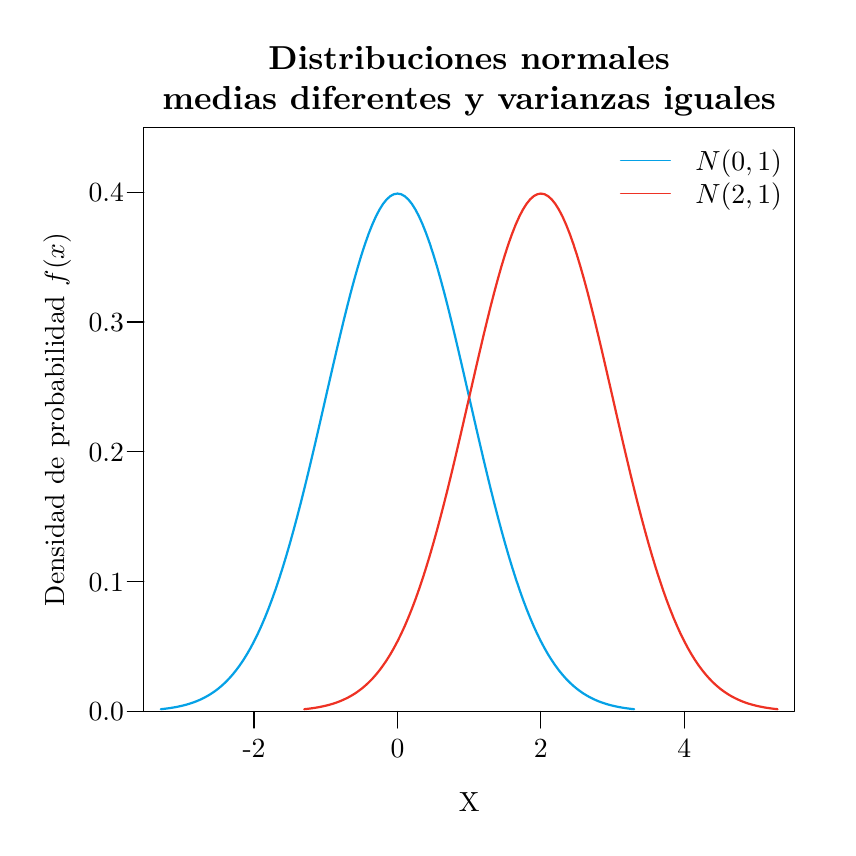
\begin{tikzpicture}[x=1pt,y=1pt]
\definecolor{fillColor}{RGB}{255,255,255}
\path[use as bounding box,fill=fillColor,fill opacity=0.00] (0,0) rectangle (289.08,289.08);
\begin{scope}
\path[clip] ( 42.00, 42.00) rectangle (277.08,253.08);
\definecolor{drawColor}{RGB}{5,161,230}

\path[draw=drawColor,line width= 0.8pt,line join=round,line cap=round] ( 48.12, 42.81) --
	( 49.41, 42.95) --
	( 50.71, 43.12) --
	( 52.00, 43.31) --
	( 53.30, 43.53) --
	( 54.59, 43.79) --
	( 55.89, 44.08) --
	( 57.18, 44.41) --
	( 58.48, 44.79) --
	( 59.78, 45.22) --
	( 61.07, 45.71) --
	( 62.37, 46.27) --
	( 63.66, 46.89) --
	( 64.96, 47.59) --
	( 66.25, 48.37) --
	( 67.55, 49.25) --
	( 68.85, 50.22) --
	( 70.14, 51.31) --
	( 71.44, 52.50) --
	( 72.73, 53.83) --
	( 74.03, 55.29) --
	( 75.32, 56.89) --
	( 76.62, 58.64) --
	( 77.92, 60.55) --
	( 79.21, 62.63) --
	( 80.51, 64.89) --
	( 81.80, 67.33) --
	( 83.10, 69.95) --
	( 84.39, 72.78) --
	( 85.69, 75.80) --
	( 86.98, 79.03) --
	( 88.28, 82.47) --
	( 89.58, 86.12) --
	( 90.87, 89.97) --
	( 92.17, 94.03) --
	( 93.46, 98.29) --
	( 94.76,102.75) --
	( 96.05,107.40) --
	( 97.35,112.23) --
	( 98.65,117.23) --
	( 99.94,122.38) --
	(101.24,127.67) --
	(102.53,133.09) --
	(103.83,138.60) --
	(105.12,144.19) --
	(106.42,149.83) --
	(107.71,155.50) --
	(109.01,161.17) --
	(110.31,166.81) --
	(111.60,172.39) --
	(112.90,177.88) --
	(114.19,183.25) --
	(115.49,188.47) --
	(116.78,193.50) --
	(118.08,198.30) --
	(119.38,202.86) --
	(120.67,207.14) --
	(121.97,211.11) --
	(123.26,214.74) --
	(124.56,218.01) --
	(125.85,220.90) --
	(127.15,223.37) --
	(128.44,225.43) --
	(129.74,227.04) --
	(131.04,228.20) --
	(132.33,228.90) --
	(133.63,229.13) --
	(134.92,228.90) --
	(136.22,228.20) --
	(137.51,227.04) --
	(138.81,225.43) --
	(140.11,223.37) --
	(141.40,220.90) --
	(142.70,218.01) --
	(143.99,214.74) --
	(145.29,211.11) --
	(146.58,207.14) --
	(147.88,202.86) --
	(149.17,198.30) --
	(150.47,193.50) --
	(151.77,188.47) --
	(153.06,183.25) --
	(154.36,177.88) --
	(155.65,172.39) --
	(156.95,166.81) --
	(158.24,161.17) --
	(159.54,155.50) --
	(160.84,149.83) --
	(162.13,144.19) --
	(163.43,138.60) --
	(164.72,133.09) --
	(166.02,127.67) --
	(167.31,122.38) --
	(168.61,117.23) --
	(169.91,112.23) --
	(171.20,107.40) --
	(172.50,102.75) --
	(173.79, 98.29) --
	(175.09, 94.03) --
	(176.38, 89.97) --
	(177.68, 86.12) --
	(178.97, 82.47) --
	(180.27, 79.03) --
	(181.57, 75.80) --
	(182.86, 72.78) --
	(184.16, 69.95) --
	(185.45, 67.33) --
	(186.75, 64.89) --
	(188.04, 62.63) --
	(189.34, 60.55) --
	(190.64, 58.64) --
	(191.93, 56.89) --
	(193.23, 55.29) --
	(194.52, 53.83) --
	(195.82, 52.50) --
	(197.11, 51.31) --
	(198.41, 50.22) --
	(199.70, 49.25) --
	(201.00, 48.37) --
	(202.30, 47.59) --
	(203.59, 46.89) --
	(204.89, 46.27) --
	(206.18, 45.71) --
	(207.48, 45.22) --
	(208.77, 44.79) --
	(210.07, 44.41) --
	(211.37, 44.08) --
	(212.66, 43.79) --
	(213.96, 43.53) --
	(215.25, 43.31) --
	(216.55, 43.12) --
	(217.84, 42.95) --
	(219.14, 42.81);
\end{scope}
\begin{scope}
\path[clip] (  0.00,  0.00) rectangle (289.08,289.08);
\definecolor{drawColor}{RGB}{0,0,0}

\path[draw=drawColor,line width= 0.4pt,line join=round,line cap=round] ( 81.80, 42.00) -- (237.28, 42.00);

\path[draw=drawColor,line width= 0.4pt,line join=round,line cap=round] ( 81.80, 42.00) -- ( 81.80, 36.00);

\path[draw=drawColor,line width= 0.4pt,line join=round,line cap=round] (133.63, 42.00) -- (133.63, 36.00);

\path[draw=drawColor,line width= 0.4pt,line join=round,line cap=round] (185.45, 42.00) -- (185.45, 36.00);

\path[draw=drawColor,line width= 0.4pt,line join=round,line cap=round] (237.28, 42.00) -- (237.28, 36.00);

\node[text=drawColor,anchor=base,inner sep=0pt, outer sep=0pt, scale=  1.00] at ( 81.80, 25.20) {-2};

\node[text=drawColor,anchor=base,inner sep=0pt, outer sep=0pt, scale=  1.00] at (133.63, 25.20) {0};

\node[text=drawColor,anchor=base,inner sep=0pt, outer sep=0pt, scale=  1.00] at (185.45, 25.20) {2};

\node[text=drawColor,anchor=base,inner sep=0pt, outer sep=0pt, scale=  1.00] at (237.28, 25.20) {4};

\path[draw=drawColor,line width= 0.4pt,line join=round,line cap=round] ( 42.00, 42.00) -- ( 42.00,229.63);

\path[draw=drawColor,line width= 0.4pt,line join=round,line cap=round] ( 42.00, 42.00) -- ( 36.00, 42.00);

\path[draw=drawColor,line width= 0.4pt,line join=round,line cap=round] ( 42.00, 88.91) -- ( 36.00, 88.91);

\path[draw=drawColor,line width= 0.4pt,line join=round,line cap=round] ( 42.00,135.81) -- ( 36.00,135.81);

\path[draw=drawColor,line width= 0.4pt,line join=round,line cap=round] ( 42.00,182.72) -- ( 36.00,182.72);

\path[draw=drawColor,line width= 0.4pt,line join=round,line cap=round] ( 42.00,229.63) -- ( 36.00,229.63);

\node[text=drawColor,anchor=base east,inner sep=0pt, outer sep=0pt, scale=  1.00] at ( 34.80, 38.56) {0.0};

\node[text=drawColor,anchor=base east,inner sep=0pt, outer sep=0pt, scale=  1.00] at ( 34.80, 85.46) {0.1};

\node[text=drawColor,anchor=base east,inner sep=0pt, outer sep=0pt, scale=  1.00] at ( 34.80,132.37) {0.2};

\node[text=drawColor,anchor=base east,inner sep=0pt, outer sep=0pt, scale=  1.00] at ( 34.80,179.28) {0.3};

\node[text=drawColor,anchor=base east,inner sep=0pt, outer sep=0pt, scale=  1.00] at ( 34.80,226.18) {0.4};

\path[draw=drawColor,line width= 0.4pt,line join=round,line cap=round] ( 42.00, 42.00) --
	(277.08, 42.00) --
	(277.08,253.08) --
	( 42.00,253.08) --
	( 42.00, 42.00);
\end{scope}
\begin{scope}
\path[clip] (  0.00,  0.00) rectangle (289.08,289.08);
\definecolor{drawColor}{RGB}{0,0,0}

\node[text=drawColor,anchor=base,inner sep=0pt, outer sep=0pt, scale=  1.20] at (159.54,274.09) {\bfseries Distribuciones normales};

\node[text=drawColor,anchor=base,inner sep=0pt, outer sep=0pt, scale=  1.20] at (159.54,259.69) {\bfseries medias diferentes y varianzas iguales};

\node[text=drawColor,anchor=base,inner sep=0pt, outer sep=0pt, scale=  1.00] at (159.54,  6.00) {X};

\node[text=drawColor,rotate= 90.00,anchor=base,inner sep=0pt, outer sep=0pt, scale=  1.00] at ( 13.20,147.54) {Densidad de probabilidad $f(x)$};
\end{scope}
\begin{scope}
\path[clip] ( 42.00, 42.00) rectangle (277.08,253.08);
\definecolor{drawColor}{RGB}{238,50,36}

\path[draw=drawColor,line width= 0.8pt,line join=round,line cap=round] ( 99.94, 42.81) --
	(101.24, 42.95) --
	(102.53, 43.12) --
	(103.83, 43.31) --
	(105.12, 43.53) --
	(106.42, 43.79) --
	(107.71, 44.08) --
	(109.01, 44.41) --
	(110.31, 44.79) --
	(111.60, 45.22) --
	(112.90, 45.71) --
	(114.19, 46.27) --
	(115.49, 46.89) --
	(116.78, 47.59) --
	(118.08, 48.37) --
	(119.38, 49.25) --
	(120.67, 50.22) --
	(121.97, 51.31) --
	(123.26, 52.50) --
	(124.56, 53.83) --
	(125.85, 55.29) --
	(127.15, 56.89) --
	(128.44, 58.64) --
	(129.74, 60.55) --
	(131.04, 62.63) --
	(132.33, 64.89) --
	(133.63, 67.33) --
	(134.92, 69.95) --
	(136.22, 72.78) --
	(137.51, 75.80) --
	(138.81, 79.03) --
	(140.11, 82.47) --
	(141.40, 86.12) --
	(142.70, 89.97) --
	(143.99, 94.03) --
	(145.29, 98.29) --
	(146.58,102.75) --
	(147.88,107.40) --
	(149.17,112.23) --
	(150.47,117.23) --
	(151.77,122.38) --
	(153.06,127.67) --
	(154.36,133.09) --
	(155.65,138.60) --
	(156.95,144.19) --
	(158.24,149.83) --
	(159.54,155.50) --
	(160.84,161.17) --
	(162.13,166.81) --
	(163.43,172.39) --
	(164.72,177.88) --
	(166.02,183.25) --
	(167.31,188.47) --
	(168.61,193.50) --
	(169.91,198.30) --
	(171.20,202.86) --
	(172.50,207.14) --
	(173.79,211.11) --
	(175.09,214.74) --
	(176.38,218.01) --
	(177.68,220.90) --
	(178.97,223.37) --
	(180.27,225.43) --
	(181.57,227.04) --
	(182.86,228.20) --
	(184.16,228.90) --
	(185.45,229.13) --
	(186.75,228.90) --
	(188.04,228.20) --
	(189.34,227.04) --
	(190.64,225.43) --
	(191.93,223.37) --
	(193.23,220.90) --
	(194.52,218.01) --
	(195.82,214.74) --
	(197.11,211.11) --
	(198.41,207.14) --
	(199.70,202.86) --
	(201.00,198.30) --
	(202.30,193.50) --
	(203.59,188.47) --
	(204.89,183.25) --
	(206.18,177.88) --
	(207.48,172.39) --
	(208.77,166.81) --
	(210.07,161.17) --
	(211.37,155.50) --
	(212.66,149.83) --
	(213.96,144.19) --
	(215.25,138.60) --
	(216.55,133.09) --
	(217.84,127.67) --
	(219.14,122.38) --
	(220.43,117.23) --
	(221.73,112.23) --
	(223.03,107.40) --
	(224.32,102.75) --
	(225.62, 98.29) --
	(226.91, 94.03) --
	(228.21, 89.97) --
	(229.50, 86.12) --
	(230.80, 82.47) --
	(232.10, 79.03) --
	(233.39, 75.80) --
	(234.69, 72.78) --
	(235.98, 69.95) --
	(237.28, 67.33) --
	(238.57, 64.89) --
	(239.87, 62.63) --
	(241.16, 60.55) --
	(242.46, 58.64) --
	(243.76, 56.89) --
	(245.05, 55.29) --
	(246.35, 53.83) --
	(247.64, 52.50) --
	(248.94, 51.31) --
	(250.23, 50.22) --
	(251.53, 49.25) --
	(252.83, 48.37) --
	(254.12, 47.59) --
	(255.42, 46.89) --
	(256.71, 46.27) --
	(258.01, 45.71) --
	(259.30, 45.22) --
	(260.60, 44.79) --
	(261.90, 44.41) --
	(263.19, 44.08) --
	(264.49, 43.79) --
	(265.78, 43.53) --
	(267.08, 43.31) --
	(268.37, 43.12) --
	(269.67, 42.95) --
	(270.96, 42.81);
\definecolor{drawColor}{RGB}{5,161,230}

\path[draw=drawColor,line width= 0.4pt,line join=round,line cap=round] (214.23,241.08) -- (232.23,241.08);
\definecolor{drawColor}{RGB}{238,50,36}

\path[draw=drawColor,line width= 0.4pt,line join=round,line cap=round] (214.23,229.08) -- (232.23,229.08);
\definecolor{drawColor}{RGB}{0,0,0}

\node[text=drawColor,anchor=base west,inner sep=0pt, outer sep=0pt, scale=  1.00] at (241.23,237.64) {$N(0,1)$};

\node[text=drawColor,anchor=base west,inner sep=0pt, outer sep=0pt, scale=  1.00] at (241.23,225.64) {$N(2,1)$};
\end{scope}
\end{tikzpicture}
}
	\tikzsetnextfilename{variables_aleatorias_continuas/funcion_densidad_normal_varianzas_diferentes}
	\resizebox{0.5\textwidth}{!}{% Created by tikzDevice version 0.10.1 on 2016-05-08 18:26:50
% !TEX encoding = UTF-8 Unicode
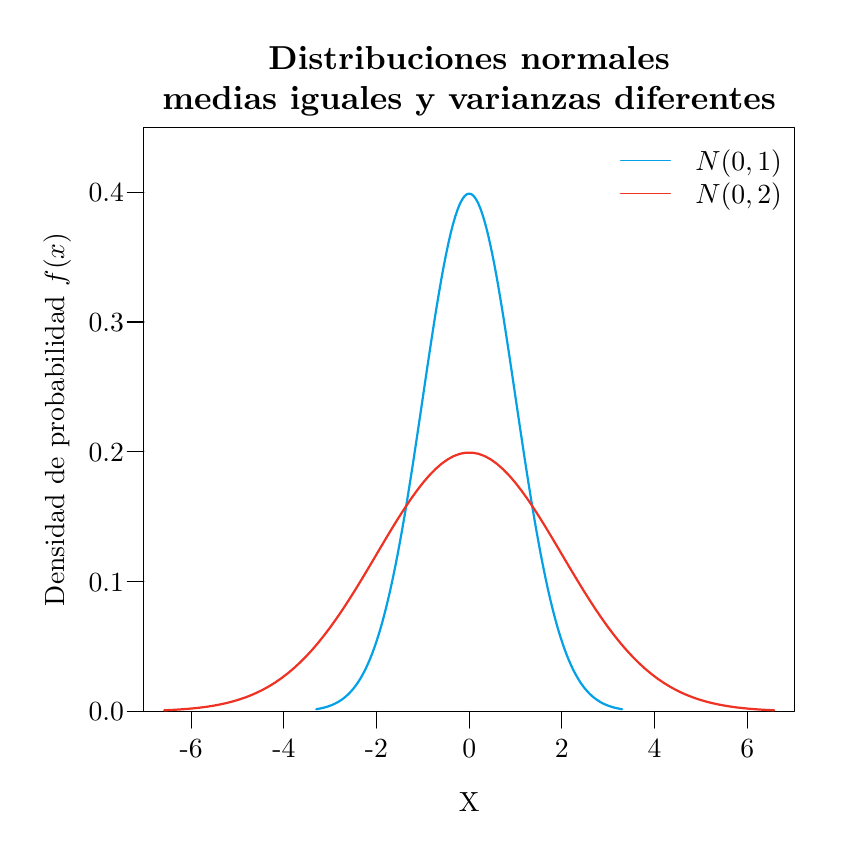
\begin{tikzpicture}[x=1pt,y=1pt]
\definecolor{fillColor}{RGB}{255,255,255}
\path[use as bounding box,fill=fillColor,fill opacity=0.00] (0,0) rectangle (289.08,289.08);
\begin{scope}
\path[clip] ( 42.00, 42.00) rectangle (277.08,253.08);
\definecolor{drawColor}{RGB}{5,161,230}

\path[draw=drawColor,line width= 0.8pt,line join=round,line cap=round] (104.29, 42.81) --
	(105.12, 42.95) --
	(105.96, 43.12) --
	(106.80, 43.31) --
	(107.63, 43.53) --
	(108.47, 43.79) --
	(109.31, 44.08) --
	(110.15, 44.41) --
	(110.98, 44.79) --
	(111.82, 45.22) --
	(112.66, 45.71) --
	(113.50, 46.27) --
	(114.33, 46.89) --
	(115.17, 47.59) --
	(116.01, 48.37) --
	(116.84, 49.25) --
	(117.68, 50.22) --
	(118.52, 51.31) --
	(119.36, 52.50) --
	(120.19, 53.83) --
	(121.03, 55.29) --
	(121.87, 56.89) --
	(122.70, 58.64) --
	(123.54, 60.55) --
	(124.38, 62.63) --
	(125.22, 64.89) --
	(126.05, 67.33) --
	(126.89, 69.95) --
	(127.73, 72.78) --
	(128.56, 75.80) --
	(129.40, 79.03) --
	(130.24, 82.47) --
	(131.08, 86.12) --
	(131.91, 89.97) --
	(132.75, 94.03) --
	(133.59, 98.29) --
	(134.42,102.75) --
	(135.26,107.40) --
	(136.10,112.23) --
	(136.94,117.23) --
	(137.77,122.38) --
	(138.61,127.67) --
	(139.45,133.09) --
	(140.28,138.60) --
	(141.12,144.19) --
	(141.96,149.83) --
	(142.80,155.50) --
	(143.63,161.17) --
	(144.47,166.81) --
	(145.31,172.39) --
	(146.15,177.88) --
	(146.98,183.25) --
	(147.82,188.47) --
	(148.66,193.50) --
	(149.49,198.30) --
	(150.33,202.86) --
	(151.17,207.14) --
	(152.01,211.11) --
	(152.84,214.74) --
	(153.68,218.01) --
	(154.52,220.90) --
	(155.35,223.37) --
	(156.19,225.43) --
	(157.03,227.04) --
	(157.87,228.20) --
	(158.70,228.90) --
	(159.54,229.13) --
	(160.38,228.90) --
	(161.21,228.20) --
	(162.05,227.04) --
	(162.89,225.43) --
	(163.73,223.37) --
	(164.56,220.90) --
	(165.40,218.01) --
	(166.24,214.74) --
	(167.07,211.11) --
	(167.91,207.14) --
	(168.75,202.86) --
	(169.59,198.30) --
	(170.42,193.50) --
	(171.26,188.47) --
	(172.10,183.25) --
	(172.93,177.88) --
	(173.77,172.39) --
	(174.61,166.81) --
	(175.45,161.17) --
	(176.28,155.50) --
	(177.12,149.83) --
	(177.96,144.19) --
	(178.80,138.60) --
	(179.63,133.09) --
	(180.47,127.67) --
	(181.31,122.38) --
	(182.14,117.23) --
	(182.98,112.23) --
	(183.82,107.40) --
	(184.66,102.75) --
	(185.49, 98.29) --
	(186.33, 94.03) --
	(187.17, 89.97) --
	(188.00, 86.12) --
	(188.84, 82.47) --
	(189.68, 79.03) --
	(190.52, 75.80) --
	(191.35, 72.78) --
	(192.19, 69.95) --
	(193.03, 67.33) --
	(193.86, 64.89) --
	(194.70, 62.63) --
	(195.54, 60.55) --
	(196.38, 58.64) --
	(197.21, 56.89) --
	(198.05, 55.29) --
	(198.89, 53.83) --
	(199.72, 52.50) --
	(200.56, 51.31) --
	(201.40, 50.22) --
	(202.24, 49.25) --
	(203.07, 48.37) --
	(203.91, 47.59) --
	(204.75, 46.89) --
	(205.58, 46.27) --
	(206.42, 45.71) --
	(207.26, 45.22) --
	(208.10, 44.79) --
	(208.93, 44.41) --
	(209.77, 44.08) --
	(210.61, 43.79) --
	(211.45, 43.53) --
	(212.28, 43.31) --
	(213.12, 43.12) --
	(213.96, 42.95) --
	(214.79, 42.81);
\end{scope}
\begin{scope}
\path[clip] (  0.00,  0.00) rectangle (289.08,289.08);
\definecolor{drawColor}{RGB}{0,0,0}

\path[draw=drawColor,line width= 0.4pt,line join=round,line cap=round] ( 59.08, 42.00) -- (260.00, 42.00);

\path[draw=drawColor,line width= 0.4pt,line join=round,line cap=round] ( 59.08, 42.00) -- ( 59.08, 36.00);

\path[draw=drawColor,line width= 0.4pt,line join=round,line cap=round] ( 92.57, 42.00) -- ( 92.57, 36.00);

\path[draw=drawColor,line width= 0.4pt,line join=round,line cap=round] (126.05, 42.00) -- (126.05, 36.00);

\path[draw=drawColor,line width= 0.4pt,line join=round,line cap=round] (159.54, 42.00) -- (159.54, 36.00);

\path[draw=drawColor,line width= 0.4pt,line join=round,line cap=round] (193.03, 42.00) -- (193.03, 36.00);

\path[draw=drawColor,line width= 0.4pt,line join=round,line cap=round] (226.51, 42.00) -- (226.51, 36.00);

\path[draw=drawColor,line width= 0.4pt,line join=round,line cap=round] (260.00, 42.00) -- (260.00, 36.00);

\node[text=drawColor,anchor=base,inner sep=0pt, outer sep=0pt, scale=  1.00] at ( 59.08, 25.20) {-6};

\node[text=drawColor,anchor=base,inner sep=0pt, outer sep=0pt, scale=  1.00] at ( 92.57, 25.20) {-4};

\node[text=drawColor,anchor=base,inner sep=0pt, outer sep=0pt, scale=  1.00] at (126.05, 25.20) {-2};

\node[text=drawColor,anchor=base,inner sep=0pt, outer sep=0pt, scale=  1.00] at (159.54, 25.20) {0};

\node[text=drawColor,anchor=base,inner sep=0pt, outer sep=0pt, scale=  1.00] at (193.03, 25.20) {2};

\node[text=drawColor,anchor=base,inner sep=0pt, outer sep=0pt, scale=  1.00] at (226.51, 25.20) {4};

\node[text=drawColor,anchor=base,inner sep=0pt, outer sep=0pt, scale=  1.00] at (260.00, 25.20) {6};

\path[draw=drawColor,line width= 0.4pt,line join=round,line cap=round] ( 42.00, 42.00) -- ( 42.00,229.63);

\path[draw=drawColor,line width= 0.4pt,line join=round,line cap=round] ( 42.00, 42.00) -- ( 36.00, 42.00);

\path[draw=drawColor,line width= 0.4pt,line join=round,line cap=round] ( 42.00, 88.91) -- ( 36.00, 88.91);

\path[draw=drawColor,line width= 0.4pt,line join=round,line cap=round] ( 42.00,135.81) -- ( 36.00,135.81);

\path[draw=drawColor,line width= 0.4pt,line join=round,line cap=round] ( 42.00,182.72) -- ( 36.00,182.72);

\path[draw=drawColor,line width= 0.4pt,line join=round,line cap=round] ( 42.00,229.63) -- ( 36.00,229.63);

\node[text=drawColor,anchor=base east,inner sep=0pt, outer sep=0pt, scale=  1.00] at ( 34.80, 38.56) {0.0};

\node[text=drawColor,anchor=base east,inner sep=0pt, outer sep=0pt, scale=  1.00] at ( 34.80, 85.46) {0.1};

\node[text=drawColor,anchor=base east,inner sep=0pt, outer sep=0pt, scale=  1.00] at ( 34.80,132.37) {0.2};

\node[text=drawColor,anchor=base east,inner sep=0pt, outer sep=0pt, scale=  1.00] at ( 34.80,179.28) {0.3};

\node[text=drawColor,anchor=base east,inner sep=0pt, outer sep=0pt, scale=  1.00] at ( 34.80,226.18) {0.4};

\path[draw=drawColor,line width= 0.4pt,line join=round,line cap=round] ( 42.00, 42.00) --
	(277.08, 42.00) --
	(277.08,253.08) --
	( 42.00,253.08) --
	( 42.00, 42.00);
\end{scope}
\begin{scope}
\path[clip] (  0.00,  0.00) rectangle (289.08,289.08);
\definecolor{drawColor}{RGB}{0,0,0}

\node[text=drawColor,anchor=base,inner sep=0pt, outer sep=0pt, scale=  1.20] at (159.54,274.09) {\bfseries Distribuciones normales};

\node[text=drawColor,anchor=base,inner sep=0pt, outer sep=0pt, scale=  1.20] at (159.54,259.69) {\bfseries medias iguales y varianzas diferentes};

\node[text=drawColor,anchor=base,inner sep=0pt, outer sep=0pt, scale=  1.00] at (159.54,  6.00) {X};

\node[text=drawColor,rotate= 90.00,anchor=base,inner sep=0pt, outer sep=0pt, scale=  1.00] at ( 13.20,147.54) {Densidad de probabilidad $f(x)$};
\end{scope}
\begin{scope}
\path[clip] ( 42.00, 42.00) rectangle (277.08,253.08);
\definecolor{drawColor}{RGB}{238,50,36}

\path[draw=drawColor,line width= 0.8pt,line join=round,line cap=round] ( 49.35, 42.42) --
	( 51.58, 42.52) --
	( 53.80, 42.64) --
	( 56.03, 42.79) --
	( 58.25, 42.97) --
	( 60.48, 43.18) --
	( 62.71, 43.43) --
	( 64.93, 43.73) --
	( 67.16, 44.08) --
	( 69.38, 44.50) --
	( 71.61, 44.98) --
	( 73.84, 45.54) --
	( 76.06, 46.19) --
	( 78.29, 46.93) --
	( 80.52, 47.78) --
	( 82.74, 48.75) --
	( 84.97, 49.84) --
	( 87.19, 51.07) --
	( 89.42, 52.45) --
	( 91.65, 53.98) --
	( 93.87, 55.68) --
	( 96.10, 57.55) --
	( 98.32, 59.60) --
	(100.55, 61.83) --
	(102.78, 64.24) --
	(105.00, 66.84) --
	(107.23, 69.62) --
	(109.45, 72.57) --
	(111.68, 75.69) --
	(113.91, 78.97) --
	(116.13, 82.39) --
	(118.36, 85.92) --
	(120.58, 89.56) --
	(122.81, 93.27) --
	(125.04, 97.03) --
	(127.26,100.80) --
	(129.49,104.55) --
	(131.71,108.25) --
	(133.94,111.86) --
	(136.17,115.34) --
	(138.39,118.65) --
	(140.62,121.76) --
	(142.84,124.63) --
	(145.07,127.23) --
	(147.30,129.52) --
	(149.52,131.47) --
	(151.75,133.07) --
	(153.97,134.28) --
	(156.20,135.10) --
	(158.43,135.51) --
	(160.65,135.51) --
	(162.88,135.10) --
	(165.11,134.28) --
	(167.33,133.07) --
	(169.56,131.47) --
	(171.78,129.52) --
	(174.01,127.23) --
	(176.24,124.63) --
	(178.46,121.76) --
	(180.69,118.65) --
	(182.91,115.34) --
	(185.14,111.86) --
	(187.37,108.25) --
	(189.59,104.55) --
	(191.82,100.80) --
	(194.04, 97.03) --
	(196.27, 93.27) --
	(198.50, 89.56) --
	(200.72, 85.92) --
	(202.95, 82.39) --
	(205.17, 78.97) --
	(207.40, 75.69) --
	(209.63, 72.57) --
	(211.85, 69.62) --
	(214.08, 66.84) --
	(216.30, 64.24) --
	(218.53, 61.83) --
	(220.76, 59.60) --
	(222.98, 57.55) --
	(225.21, 55.68) --
	(227.43, 53.98) --
	(229.66, 52.45) --
	(231.89, 51.07) --
	(234.11, 49.84) --
	(236.34, 48.75) --
	(238.56, 47.78) --
	(240.79, 46.93) --
	(243.02, 46.19) --
	(245.24, 45.54) --
	(247.47, 44.98) --
	(249.70, 44.50) --
	(251.92, 44.08) --
	(254.15, 43.73) --
	(256.37, 43.43) --
	(258.60, 43.18) --
	(260.83, 42.97) --
	(263.05, 42.79) --
	(265.28, 42.64) --
	(267.50, 42.52) --
	(269.73, 42.42);
\definecolor{drawColor}{RGB}{5,161,230}

\path[draw=drawColor,line width= 0.4pt,line join=round,line cap=round] (214.23,241.08) -- (232.23,241.08);
\definecolor{drawColor}{RGB}{238,50,36}

\path[draw=drawColor,line width= 0.4pt,line join=round,line cap=round] (214.23,229.08) -- (232.23,229.08);
\definecolor{drawColor}{RGB}{0,0,0}

\node[text=drawColor,anchor=base west,inner sep=0pt, outer sep=0pt, scale=  1.00] at (241.23,237.64) {$N(0,1)$};

\node[text=drawColor,anchor=base west,inner sep=0pt, outer sep=0pt, scale=  1.00] at (241.23,225.64) {$N(0,2)$};
\end{scope}
\end{tikzpicture}
}
	}
	\mode<presentation>{\resizebox{\textwidth}{!}{% Created by tikzDevice version 0.10.1 on 2016-05-08 18:26:50
% !TEX encoding = UTF-8 Unicode
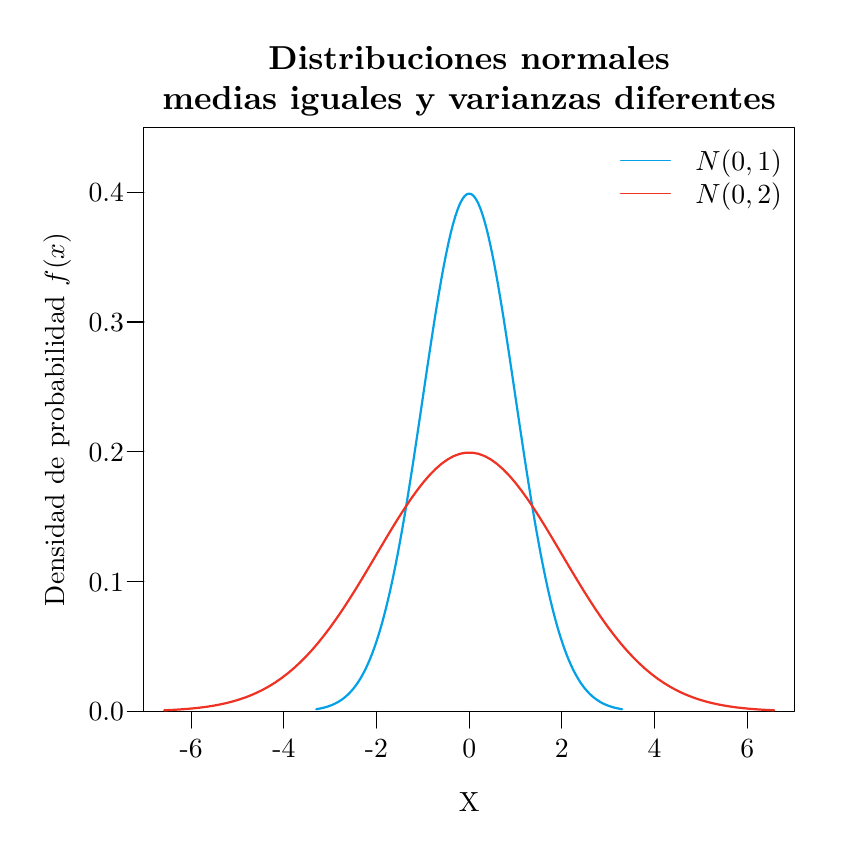
\begin{tikzpicture}[x=1pt,y=1pt]
\definecolor{fillColor}{RGB}{255,255,255}
\path[use as bounding box,fill=fillColor,fill opacity=0.00] (0,0) rectangle (289.08,289.08);
\begin{scope}
\path[clip] ( 42.00, 42.00) rectangle (277.08,253.08);
\definecolor{drawColor}{RGB}{5,161,230}

\path[draw=drawColor,line width= 0.8pt,line join=round,line cap=round] (104.29, 42.81) --
	(105.12, 42.95) --
	(105.96, 43.12) --
	(106.80, 43.31) --
	(107.63, 43.53) --
	(108.47, 43.79) --
	(109.31, 44.08) --
	(110.15, 44.41) --
	(110.98, 44.79) --
	(111.82, 45.22) --
	(112.66, 45.71) --
	(113.50, 46.27) --
	(114.33, 46.89) --
	(115.17, 47.59) --
	(116.01, 48.37) --
	(116.84, 49.25) --
	(117.68, 50.22) --
	(118.52, 51.31) --
	(119.36, 52.50) --
	(120.19, 53.83) --
	(121.03, 55.29) --
	(121.87, 56.89) --
	(122.70, 58.64) --
	(123.54, 60.55) --
	(124.38, 62.63) --
	(125.22, 64.89) --
	(126.05, 67.33) --
	(126.89, 69.95) --
	(127.73, 72.78) --
	(128.56, 75.80) --
	(129.40, 79.03) --
	(130.24, 82.47) --
	(131.08, 86.12) --
	(131.91, 89.97) --
	(132.75, 94.03) --
	(133.59, 98.29) --
	(134.42,102.75) --
	(135.26,107.40) --
	(136.10,112.23) --
	(136.94,117.23) --
	(137.77,122.38) --
	(138.61,127.67) --
	(139.45,133.09) --
	(140.28,138.60) --
	(141.12,144.19) --
	(141.96,149.83) --
	(142.80,155.50) --
	(143.63,161.17) --
	(144.47,166.81) --
	(145.31,172.39) --
	(146.15,177.88) --
	(146.98,183.25) --
	(147.82,188.47) --
	(148.66,193.50) --
	(149.49,198.30) --
	(150.33,202.86) --
	(151.17,207.14) --
	(152.01,211.11) --
	(152.84,214.74) --
	(153.68,218.01) --
	(154.52,220.90) --
	(155.35,223.37) --
	(156.19,225.43) --
	(157.03,227.04) --
	(157.87,228.20) --
	(158.70,228.90) --
	(159.54,229.13) --
	(160.38,228.90) --
	(161.21,228.20) --
	(162.05,227.04) --
	(162.89,225.43) --
	(163.73,223.37) --
	(164.56,220.90) --
	(165.40,218.01) --
	(166.24,214.74) --
	(167.07,211.11) --
	(167.91,207.14) --
	(168.75,202.86) --
	(169.59,198.30) --
	(170.42,193.50) --
	(171.26,188.47) --
	(172.10,183.25) --
	(172.93,177.88) --
	(173.77,172.39) --
	(174.61,166.81) --
	(175.45,161.17) --
	(176.28,155.50) --
	(177.12,149.83) --
	(177.96,144.19) --
	(178.80,138.60) --
	(179.63,133.09) --
	(180.47,127.67) --
	(181.31,122.38) --
	(182.14,117.23) --
	(182.98,112.23) --
	(183.82,107.40) --
	(184.66,102.75) --
	(185.49, 98.29) --
	(186.33, 94.03) --
	(187.17, 89.97) --
	(188.00, 86.12) --
	(188.84, 82.47) --
	(189.68, 79.03) --
	(190.52, 75.80) --
	(191.35, 72.78) --
	(192.19, 69.95) --
	(193.03, 67.33) --
	(193.86, 64.89) --
	(194.70, 62.63) --
	(195.54, 60.55) --
	(196.38, 58.64) --
	(197.21, 56.89) --
	(198.05, 55.29) --
	(198.89, 53.83) --
	(199.72, 52.50) --
	(200.56, 51.31) --
	(201.40, 50.22) --
	(202.24, 49.25) --
	(203.07, 48.37) --
	(203.91, 47.59) --
	(204.75, 46.89) --
	(205.58, 46.27) --
	(206.42, 45.71) --
	(207.26, 45.22) --
	(208.10, 44.79) --
	(208.93, 44.41) --
	(209.77, 44.08) --
	(210.61, 43.79) --
	(211.45, 43.53) --
	(212.28, 43.31) --
	(213.12, 43.12) --
	(213.96, 42.95) --
	(214.79, 42.81);
\end{scope}
\begin{scope}
\path[clip] (  0.00,  0.00) rectangle (289.08,289.08);
\definecolor{drawColor}{RGB}{0,0,0}

\path[draw=drawColor,line width= 0.4pt,line join=round,line cap=round] ( 59.08, 42.00) -- (260.00, 42.00);

\path[draw=drawColor,line width= 0.4pt,line join=round,line cap=round] ( 59.08, 42.00) -- ( 59.08, 36.00);

\path[draw=drawColor,line width= 0.4pt,line join=round,line cap=round] ( 92.57, 42.00) -- ( 92.57, 36.00);

\path[draw=drawColor,line width= 0.4pt,line join=round,line cap=round] (126.05, 42.00) -- (126.05, 36.00);

\path[draw=drawColor,line width= 0.4pt,line join=round,line cap=round] (159.54, 42.00) -- (159.54, 36.00);

\path[draw=drawColor,line width= 0.4pt,line join=round,line cap=round] (193.03, 42.00) -- (193.03, 36.00);

\path[draw=drawColor,line width= 0.4pt,line join=round,line cap=round] (226.51, 42.00) -- (226.51, 36.00);

\path[draw=drawColor,line width= 0.4pt,line join=round,line cap=round] (260.00, 42.00) -- (260.00, 36.00);

\node[text=drawColor,anchor=base,inner sep=0pt, outer sep=0pt, scale=  1.00] at ( 59.08, 25.20) {-6};

\node[text=drawColor,anchor=base,inner sep=0pt, outer sep=0pt, scale=  1.00] at ( 92.57, 25.20) {-4};

\node[text=drawColor,anchor=base,inner sep=0pt, outer sep=0pt, scale=  1.00] at (126.05, 25.20) {-2};

\node[text=drawColor,anchor=base,inner sep=0pt, outer sep=0pt, scale=  1.00] at (159.54, 25.20) {0};

\node[text=drawColor,anchor=base,inner sep=0pt, outer sep=0pt, scale=  1.00] at (193.03, 25.20) {2};

\node[text=drawColor,anchor=base,inner sep=0pt, outer sep=0pt, scale=  1.00] at (226.51, 25.20) {4};

\node[text=drawColor,anchor=base,inner sep=0pt, outer sep=0pt, scale=  1.00] at (260.00, 25.20) {6};

\path[draw=drawColor,line width= 0.4pt,line join=round,line cap=round] ( 42.00, 42.00) -- ( 42.00,229.63);

\path[draw=drawColor,line width= 0.4pt,line join=round,line cap=round] ( 42.00, 42.00) -- ( 36.00, 42.00);

\path[draw=drawColor,line width= 0.4pt,line join=round,line cap=round] ( 42.00, 88.91) -- ( 36.00, 88.91);

\path[draw=drawColor,line width= 0.4pt,line join=round,line cap=round] ( 42.00,135.81) -- ( 36.00,135.81);

\path[draw=drawColor,line width= 0.4pt,line join=round,line cap=round] ( 42.00,182.72) -- ( 36.00,182.72);

\path[draw=drawColor,line width= 0.4pt,line join=round,line cap=round] ( 42.00,229.63) -- ( 36.00,229.63);

\node[text=drawColor,anchor=base east,inner sep=0pt, outer sep=0pt, scale=  1.00] at ( 34.80, 38.56) {0.0};

\node[text=drawColor,anchor=base east,inner sep=0pt, outer sep=0pt, scale=  1.00] at ( 34.80, 85.46) {0.1};

\node[text=drawColor,anchor=base east,inner sep=0pt, outer sep=0pt, scale=  1.00] at ( 34.80,132.37) {0.2};

\node[text=drawColor,anchor=base east,inner sep=0pt, outer sep=0pt, scale=  1.00] at ( 34.80,179.28) {0.3};

\node[text=drawColor,anchor=base east,inner sep=0pt, outer sep=0pt, scale=  1.00] at ( 34.80,226.18) {0.4};

\path[draw=drawColor,line width= 0.4pt,line join=round,line cap=round] ( 42.00, 42.00) --
	(277.08, 42.00) --
	(277.08,253.08) --
	( 42.00,253.08) --
	( 42.00, 42.00);
\end{scope}
\begin{scope}
\path[clip] (  0.00,  0.00) rectangle (289.08,289.08);
\definecolor{drawColor}{RGB}{0,0,0}

\node[text=drawColor,anchor=base,inner sep=0pt, outer sep=0pt, scale=  1.20] at (159.54,274.09) {\bfseries Distribuciones normales};

\node[text=drawColor,anchor=base,inner sep=0pt, outer sep=0pt, scale=  1.20] at (159.54,259.69) {\bfseries medias iguales y varianzas diferentes};

\node[text=drawColor,anchor=base,inner sep=0pt, outer sep=0pt, scale=  1.00] at (159.54,  6.00) {X};

\node[text=drawColor,rotate= 90.00,anchor=base,inner sep=0pt, outer sep=0pt, scale=  1.00] at ( 13.20,147.54) {Densidad de probabilidad $f(x)$};
\end{scope}
\begin{scope}
\path[clip] ( 42.00, 42.00) rectangle (277.08,253.08);
\definecolor{drawColor}{RGB}{238,50,36}

\path[draw=drawColor,line width= 0.8pt,line join=round,line cap=round] ( 49.35, 42.42) --
	( 51.58, 42.52) --
	( 53.80, 42.64) --
	( 56.03, 42.79) --
	( 58.25, 42.97) --
	( 60.48, 43.18) --
	( 62.71, 43.43) --
	( 64.93, 43.73) --
	( 67.16, 44.08) --
	( 69.38, 44.50) --
	( 71.61, 44.98) --
	( 73.84, 45.54) --
	( 76.06, 46.19) --
	( 78.29, 46.93) --
	( 80.52, 47.78) --
	( 82.74, 48.75) --
	( 84.97, 49.84) --
	( 87.19, 51.07) --
	( 89.42, 52.45) --
	( 91.65, 53.98) --
	( 93.87, 55.68) --
	( 96.10, 57.55) --
	( 98.32, 59.60) --
	(100.55, 61.83) --
	(102.78, 64.24) --
	(105.00, 66.84) --
	(107.23, 69.62) --
	(109.45, 72.57) --
	(111.68, 75.69) --
	(113.91, 78.97) --
	(116.13, 82.39) --
	(118.36, 85.92) --
	(120.58, 89.56) --
	(122.81, 93.27) --
	(125.04, 97.03) --
	(127.26,100.80) --
	(129.49,104.55) --
	(131.71,108.25) --
	(133.94,111.86) --
	(136.17,115.34) --
	(138.39,118.65) --
	(140.62,121.76) --
	(142.84,124.63) --
	(145.07,127.23) --
	(147.30,129.52) --
	(149.52,131.47) --
	(151.75,133.07) --
	(153.97,134.28) --
	(156.20,135.10) --
	(158.43,135.51) --
	(160.65,135.51) --
	(162.88,135.10) --
	(165.11,134.28) --
	(167.33,133.07) --
	(169.56,131.47) --
	(171.78,129.52) --
	(174.01,127.23) --
	(176.24,124.63) --
	(178.46,121.76) --
	(180.69,118.65) --
	(182.91,115.34) --
	(185.14,111.86) --
	(187.37,108.25) --
	(189.59,104.55) --
	(191.82,100.80) --
	(194.04, 97.03) --
	(196.27, 93.27) --
	(198.50, 89.56) --
	(200.72, 85.92) --
	(202.95, 82.39) --
	(205.17, 78.97) --
	(207.40, 75.69) --
	(209.63, 72.57) --
	(211.85, 69.62) --
	(214.08, 66.84) --
	(216.30, 64.24) --
	(218.53, 61.83) --
	(220.76, 59.60) --
	(222.98, 57.55) --
	(225.21, 55.68) --
	(227.43, 53.98) --
	(229.66, 52.45) --
	(231.89, 51.07) --
	(234.11, 49.84) --
	(236.34, 48.75) --
	(238.56, 47.78) --
	(240.79, 46.93) --
	(243.02, 46.19) --
	(245.24, 45.54) --
	(247.47, 44.98) --
	(249.70, 44.50) --
	(251.92, 44.08) --
	(254.15, 43.73) --
	(256.37, 43.43) --
	(258.60, 43.18) --
	(260.83, 42.97) --
	(263.05, 42.79) --
	(265.28, 42.64) --
	(267.50, 42.52) --
	(269.73, 42.42);
\definecolor{drawColor}{RGB}{5,161,230}

\path[draw=drawColor,line width= 0.4pt,line join=round,line cap=round] (214.23,241.08) -- (232.23,241.08);
\definecolor{drawColor}{RGB}{238,50,36}

\path[draw=drawColor,line width= 0.4pt,line join=round,line cap=round] (214.23,229.08) -- (232.23,229.08);
\definecolor{drawColor}{RGB}{0,0,0}

\node[text=drawColor,anchor=base west,inner sep=0pt, outer sep=0pt, scale=  1.00] at (241.23,237.64) {$N(0,1)$};

\node[text=drawColor,anchor=base west,inner sep=0pt, outer sep=0pt, scale=  1.00] at (241.23,225.64) {$N(0,2)$};
\end{scope}
\end{tikzpicture}
}}
\end{column}
\end{columns}

\note{
La forma de la campana de Gauss depende de sus dos parámetros:
\begin{itemize}
\item Por un lado, ya hemos visto que la media $\mu$ determina dónde está centrada. En la gráfica de la izquierda podemos ver las funciones
de densidad de dos normales, una con media 0 y desviación típica 1, y otra con media 2 y desviación típica 1. Como se ve, ambas gráficas son
idénticas, salvo que la primera está centrada en el 0 y la segunda en el 2.
\item Por otro lado, la desviación típica $\sigma$, al ser una medida de la dispersión de la población, determina su anchura. En la gráfica
de la derecha podemos ver las funciones de densidad de dos normales con la misma media 0, y desviaciones típicas 1, y 2 respectivamente.
Como se ve, ambas están centradas en el 0, pero la primera es más estrecha que la segunda al tener menos dispersión. 
\end{itemize} 
}
\end{frame}


%---------------------------------------------------------------------slide----
\begin{frame}
\frametitle{Función de distribución de la Normal}
La gráfica de la función de distribución tiene forma de S. 
\begin{center}
	\tikzsetnextfilename{variables_aleatorias_continuas/funcion_distribucion_normal}
	\mode<article>{\resizebox{0.6\textwidth}{!}{%% Input file name: funcion_distribucion_normal_estandar.fig
%% FIG version: 3.2
%% Orientation: Landscape
%% Justification: Flush Left
%% Units: Inches
%% Paper size: A4
%% Magnification: 100.0
%% Resolution: 1200ppi
%% Include the following in the preamble:
%% \usepackage{textcomp}
%% End

\begin{pspicture}(6.69cm,3.44cm)(16.66cm,13.45cm)
\psset{unit=0.8cm}
%%
%% Depth: 2147483647
%%
\newgray{mycolor0}{0.74}\definecolor{mycolor0}{gray}{0.74}
\newrgbcolor{mycolor1}{1.00 0.50 0.31}\definecolor{mycolor1}{rgb}{1.00,0.50,0.31}
%%
%% Depth: 100
%%
\psset{linestyle=solid,linewidth=0.03175,linecolor=mycolor1,fillstyle=none}
\psline(10.61,6.75)(10.70,6.76)(10.80,6.76)(10.89,6.76)(10.99,6.76)(11.08,6.76)(11.17,6.77)(11.27,6.77)(11.36,6.78)(11.46,6.78)(11.55,6.79)(11.64,6.79)(11.74,6.80)(11.83,6.81)(11.93,6.83)(12.02,6.84)(12.12,6.86)(12.21,6.88)(12.30,6.90)(12.40,6.92)(12.49,6.95)(12.59,6.99)(12.68,7.03)(12.78,7.07)(12.87,7.12)(12.96,7.17)(13.06,7.23)(13.15,7.30)(13.25,7.37)(13.34,7.46)(13.43,7.55)(13.53,7.64)(13.62,7.75)(13.72,7.86)(13.81,7.99)(13.91,8.12)(14.00,8.26)(14.09,8.41)(14.19,8.56)(14.28,8.73)(14.38,8.90)(14.47,9.08)(14.56,9.27)(14.66,9.47)(14.76,9.67)(14.85,9.87)(14.94,10.08)(15.04,10.29)(15.13,10.51)(15.23,10.72)(15.32,10.94)(15.41,11.15)(15.51,11.37)(15.60,11.58)(15.70,11.79)(15.79,12.00)(15.89,12.20)(15.98,12.39)(16.07,12.58)(16.17,12.76)(16.26,12.93)(16.36,13.10)(16.45,13.26)(16.54,13.40)(16.64,13.54)(16.73,13.68)(16.83,13.80)(16.92,13.91)(17.02,14.02)(17.11,14.12)(17.20,14.21)(17.30,14.29)(17.39,14.36)(17.49,14.43)(17.58,14.49)(17.68,14.55)(17.77,14.59)(17.86,14.64)(17.96,14.67)(18.05,14.71)(18.15,14.74)(18.24,14.76)(18.33,14.79)(18.43,14.81)(18.52,14.82)(18.62,14.84)(18.71,14.85)(18.81,14.86)(18.90,14.87)(18.99,14.88)(19.09,14.88)(19.18,14.89)(19.28,14.89)(19.37,14.90)(19.47,14.90)(19.56,14.90)(19.66,14.90)(19.75,14.91)(19.84,14.91)(19.94,14.91)
\psset{linecolor=black}
\psline(11.02,6.43)(19.52,6.43)
\psline(15.27,6.43)(15.27,6.22)
\rput(15.27,5.67){$\mu$}
\psline(10.23,6.75)(10.23,14.91)
\psline(10.23,6.75)(10.02,6.75)
\psline(10.23,8.38)(10.02,8.38)
\psline(10.23,10.02)(10.02,10.02)
\psline(10.23,11.65)(10.02,11.65)
\psline(10.23,13.28)(10.02,13.28)
\psline(10.23,14.91)(10.02,14.91)
\rput{90}(9.73,6.75){0.0}
\rput{90}(9.73,8.38){0.2}
\rput{90}(9.73,10.02){0.4}
\rput{90}(9.73,11.65){0.6}
\rput{90}(9.73,13.28){0.8}
\rput{90}(9.73,14.91){1.0}
\psline(10.23,6.43)(20.31,6.43)(20.31,15.23)(10.23,15.23)(10.23,6.43)
\rput[l](12.14,15.99){Distribución normal $N(\mu,\sigma)$}
\rput(15.27,4.82){$X$}
\rput[l]{90}(8.88,8.51){Probabilidad acumulada $F(x)$}
\psset{linecolor=mycolor0}
\psline(10.23,6.75)(20.31,6.75)
\end{pspicture}
%% End
}}
	\mode<presentation>{\resizebox{0.6\textwidth}{!}{%% Input file name: funcion_distribucion_normal_estandar.fig
%% FIG version: 3.2
%% Orientation: Landscape
%% Justification: Flush Left
%% Units: Inches
%% Paper size: A4
%% Magnification: 100.0
%% Resolution: 1200ppi
%% Include the following in the preamble:
%% \usepackage{textcomp}
%% End

\begin{pspicture}(6.69cm,3.44cm)(16.66cm,13.45cm)
\psset{unit=0.8cm}
%%
%% Depth: 2147483647
%%
\newgray{mycolor0}{0.74}\definecolor{mycolor0}{gray}{0.74}
\newrgbcolor{mycolor1}{1.00 0.50 0.31}\definecolor{mycolor1}{rgb}{1.00,0.50,0.31}
%%
%% Depth: 100
%%
\psset{linestyle=solid,linewidth=0.03175,linecolor=mycolor1,fillstyle=none}
\psline(10.61,6.75)(10.70,6.76)(10.80,6.76)(10.89,6.76)(10.99,6.76)(11.08,6.76)(11.17,6.77)(11.27,6.77)(11.36,6.78)(11.46,6.78)(11.55,6.79)(11.64,6.79)(11.74,6.80)(11.83,6.81)(11.93,6.83)(12.02,6.84)(12.12,6.86)(12.21,6.88)(12.30,6.90)(12.40,6.92)(12.49,6.95)(12.59,6.99)(12.68,7.03)(12.78,7.07)(12.87,7.12)(12.96,7.17)(13.06,7.23)(13.15,7.30)(13.25,7.37)(13.34,7.46)(13.43,7.55)(13.53,7.64)(13.62,7.75)(13.72,7.86)(13.81,7.99)(13.91,8.12)(14.00,8.26)(14.09,8.41)(14.19,8.56)(14.28,8.73)(14.38,8.90)(14.47,9.08)(14.56,9.27)(14.66,9.47)(14.76,9.67)(14.85,9.87)(14.94,10.08)(15.04,10.29)(15.13,10.51)(15.23,10.72)(15.32,10.94)(15.41,11.15)(15.51,11.37)(15.60,11.58)(15.70,11.79)(15.79,12.00)(15.89,12.20)(15.98,12.39)(16.07,12.58)(16.17,12.76)(16.26,12.93)(16.36,13.10)(16.45,13.26)(16.54,13.40)(16.64,13.54)(16.73,13.68)(16.83,13.80)(16.92,13.91)(17.02,14.02)(17.11,14.12)(17.20,14.21)(17.30,14.29)(17.39,14.36)(17.49,14.43)(17.58,14.49)(17.68,14.55)(17.77,14.59)(17.86,14.64)(17.96,14.67)(18.05,14.71)(18.15,14.74)(18.24,14.76)(18.33,14.79)(18.43,14.81)(18.52,14.82)(18.62,14.84)(18.71,14.85)(18.81,14.86)(18.90,14.87)(18.99,14.88)(19.09,14.88)(19.18,14.89)(19.28,14.89)(19.37,14.90)(19.47,14.90)(19.56,14.90)(19.66,14.90)(19.75,14.91)(19.84,14.91)(19.94,14.91)
\psset{linecolor=black}
\psline(11.02,6.43)(19.52,6.43)
\psline(15.27,6.43)(15.27,6.22)
\rput(15.27,5.67){$\mu$}
\psline(10.23,6.75)(10.23,14.91)
\psline(10.23,6.75)(10.02,6.75)
\psline(10.23,8.38)(10.02,8.38)
\psline(10.23,10.02)(10.02,10.02)
\psline(10.23,11.65)(10.02,11.65)
\psline(10.23,13.28)(10.02,13.28)
\psline(10.23,14.91)(10.02,14.91)
\rput{90}(9.73,6.75){0.0}
\rput{90}(9.73,8.38){0.2}
\rput{90}(9.73,10.02){0.4}
\rput{90}(9.73,11.65){0.6}
\rput{90}(9.73,13.28){0.8}
\rput{90}(9.73,14.91){1.0}
\psline(10.23,6.43)(20.31,6.43)(20.31,15.23)(10.23,15.23)(10.23,6.43)
\rput[l](12.14,15.99){Distribución normal $N(\mu,\sigma)$}
\rput(15.27,4.82){$X$}
\rput[l]{90}(8.88,8.51){Probabilidad acumulada $F(x)$}
\psset{linecolor=mycolor0}
\psline(10.23,6.75)(20.31,6.75)
\end{pspicture}
%% End
}}
\end{center}

\note{
Por su parte, la gráfica de la función de distribución de una normal siempre tiene forma de S. 
}
\end{frame}


%---------------------------------------------------------------------slide----
\begin{frame}
\frametitle{Propiedades de la distribución Normal}
\begin{itemize}
\item La función de densidad es simétrica respecto a la media y por tanto, su coeficiente de asimetría es $g_1=0$.
\item También es mesocúrtica, ya que la función de densidad tiene forma de campana de Gauss, y por tanto, su coeficiente de apuntamiento vale $g_2=0$.
\item La media, la mediana y la moda coinciden
\[
\mu = Me = Mo.
\]
\item Tiende asintóticamente a 0 cuando $x$ tiende a $\pm \infty$.
\end{itemize}

\note{
La distribución normal tiene propiedades muy interesantes:
\begin{itemize}
\item La función de densidad es simétrica respecto a la media y por tanto, su coeficiente de asimetría es $g_1=0$.
\item También es mesocúrtica, y por tanto, su coeficiente de apuntamiento vale $g_2=0$. Recordemos que el apuntamiento de cualquier variable
se compara precisamente con el apuntamiento de la distribución normal, ya que al ser esta la distribución más común, se toma como
referencia.
\item De nuevo, al ser simétrica con respecto a la media, hasta la media tendremos acumulada la mitad de la probabilidad, y por tanto la
media coincide con la mediana, y también con la moda, ya que sobre la media se alcanza el máximo de la función de densidad.
\[
\mu = Me = Mo.
\]
\item Tiende asintóticamente a 0 cuando $x$ tiende a $\pm \infty$.
\end{itemize}
}
\end{frame}


%---------------------------------------------------------------------slide----
\begin{frame}
\frametitle{Propiedades de la distribución Normal}
\begin{center}
	\onslide<2->{$P(\mu-\sigma \leq X \leq \mu+\sigma) = 0.68$,}\\
	\onslide<3->{$P(\mu-2\sigma \leq X \leq \mu+2\sigma) = 0.95$,}\\
	\onslide<4->{$P(\mu-3\sigma \leq X \leq \mu+3\sigma) = 0.99$.}
	\mode<article>{
	\tikzsetnextfilename{variables_aleatorias_continuas/intervalo_normal_68}
	\resizebox{0.33\textwidth}{!}{% Created by tikzDevice version 0.10.1 on 2016-05-10 09:59:36
% !TEX encoding = UTF-8 Unicode
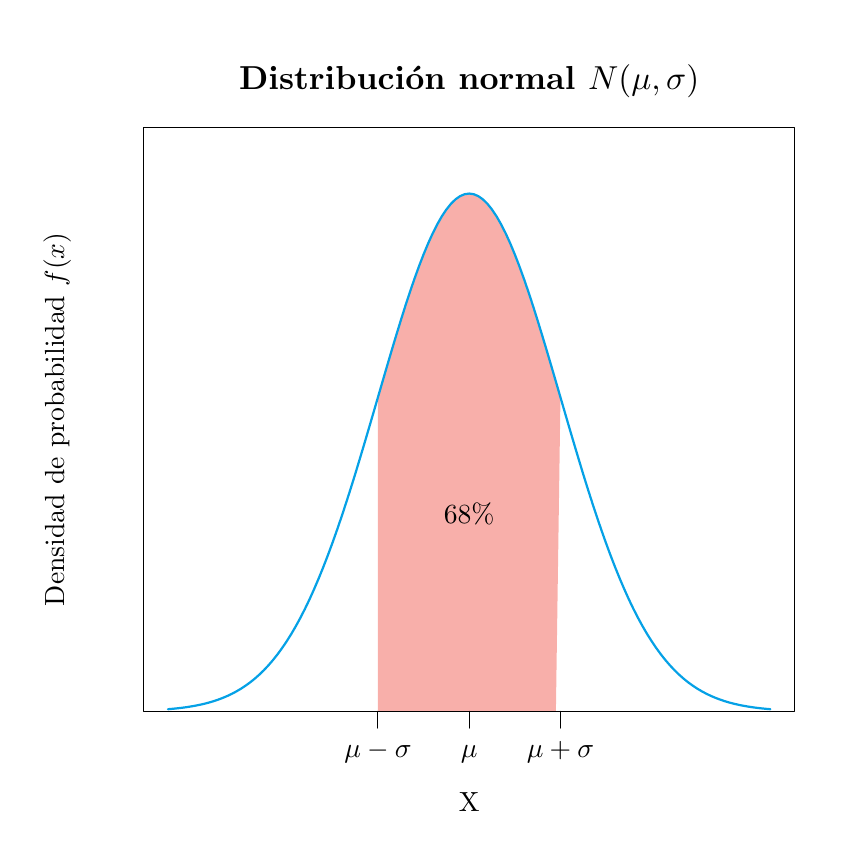
\begin{tikzpicture}[x=1pt,y=1pt]
\definecolor{fillColor}{RGB}{255,255,255}
\path[use as bounding box,fill=fillColor,fill opacity=0.00] (0,0) rectangle (289.08,289.08);
\begin{scope}
\path[clip] (  0.00,  0.00) rectangle (289.08,289.08);
\definecolor{drawColor}{RGB}{0,0,0}

\node[text=drawColor,anchor=base,inner sep=0pt, outer sep=0pt, scale=  1.20] at (159.54,266.89) {\bfseries Distribución normal $N(\mu,\sigma)$};

\node[text=drawColor,anchor=base,inner sep=0pt, outer sep=0pt, scale=  1.00] at (159.54,  6.00) {X};

\node[text=drawColor,rotate= 90.00,anchor=base,inner sep=0pt, outer sep=0pt, scale=  1.00] at ( 13.20,147.54) {Densidad de probabilidad $f(x)$};
\end{scope}
\begin{scope}
\path[clip] (  0.00,  0.00) rectangle (289.08,289.08);
\definecolor{drawColor}{RGB}{0,0,0}

\path[draw=drawColor,line width= 0.4pt,line join=round,line cap=round] (159.54, 42.00) -- (159.54, 42.00);

\path[draw=drawColor,line width= 0.4pt,line join=round,line cap=round] (159.54, 42.00) -- (159.54, 36.00);

\node[text=drawColor,anchor=base,inner sep=0pt, outer sep=0pt, scale=  1.00] at (159.54, 25.20) {$\mu$};

\path[draw=drawColor,line width= 0.4pt,line join=round,line cap=round] (126.56, 42.00) -- (192.52, 42.00);

\path[draw=drawColor,line width= 0.4pt,line join=round,line cap=round] (126.56, 42.00) -- (126.56, 36.00);

\path[draw=drawColor,line width= 0.4pt,line join=round,line cap=round] (192.52, 42.00) -- (192.52, 36.00);

\node[text=drawColor,anchor=base,inner sep=0pt, outer sep=0pt, scale=  1.00] at (126.56, 25.20) {$\mu-\sigma$};

\node[text=drawColor,anchor=base,inner sep=0pt, outer sep=0pt, scale=  1.00] at (192.52, 25.20) {$\mu+\sigma$};
\end{scope}
\begin{scope}
\path[clip] ( 42.00, 42.00) rectangle (277.08,253.08);
\definecolor{fillColor}{RGB}{238,50,36}

\path[fill=fillColor,fill opacity=0.39] (126.56, 42.00) --
	(126.56,155.50) --
	(128.21,161.17) --
	(129.86,166.81) --
	(131.51,172.39) --
	(133.16,177.88) --
	(134.81,183.25) --
	(136.45,188.47) --
	(138.10,193.50) --
	(139.75,198.30) --
	(141.40,202.86) --
	(143.05,207.14) --
	(144.70,211.11) --
	(146.35,214.74) --
	(148.00,218.01) --
	(149.65,220.90) --
	(151.30,223.37) --
	(152.94,225.43) --
	(154.59,227.04) --
	(156.24,228.20) --
	(157.89,228.90) --
	(159.54,229.13) --
	(161.19,228.90) --
	(162.84,228.20) --
	(164.49,227.04) --
	(166.14,225.43) --
	(167.78,223.37) --
	(169.43,220.90) --
	(171.08,218.01) --
	(172.73,214.74) --
	(174.38,211.11) --
	(176.03,207.14) --
	(177.68,202.86) --
	(179.33,198.30) --
	(180.98,193.50) --
	(182.63,188.47) --
	(184.27,183.25) --
	(185.92,177.88) --
	(187.57,172.39) --
	(189.22,166.81) --
	(190.87,161.17) --
	(192.52,155.50) --
	(190.87, 42.00) --
	cycle;
\definecolor{drawColor}{RGB}{0,0,0}

\node[text=drawColor,anchor=base,inner sep=0pt, outer sep=0pt, scale=  1.00] at (159.54,109.86) {$68\%$};
\definecolor{drawColor}{RGB}{5,161,230}

\path[draw=drawColor,line width= 0.8pt,line join=round,line cap=round] ( 50.71, 42.81) --
	( 52.36, 42.95) --
	( 54.00, 43.12) --
	( 55.65, 43.31) --
	( 57.30, 43.53) --
	( 58.95, 43.79) --
	( 60.60, 44.08) --
	( 62.25, 44.41) --
	( 63.90, 44.79) --
	( 65.55, 45.22) --
	( 67.20, 45.71) --
	( 68.85, 46.27) --
	( 70.49, 46.89) --
	( 72.14, 47.59) --
	( 73.79, 48.37) --
	( 75.44, 49.25) --
	( 77.09, 50.22) --
	( 78.74, 51.31) --
	( 80.39, 52.50) --
	( 82.04, 53.83) --
	( 83.69, 55.29) --
	( 85.34, 56.89) --
	( 86.98, 58.64) --
	( 88.63, 60.55) --
	( 90.28, 62.63) --
	( 91.93, 64.89) --
	( 93.58, 67.33) --
	( 95.23, 69.95) --
	( 96.88, 72.78) --
	( 98.53, 75.80) --
	(100.18, 79.03) --
	(101.83, 82.47) --
	(103.47, 86.12) --
	(105.12, 89.97) --
	(106.77, 94.03) --
	(108.42, 98.29) --
	(110.07,102.75) --
	(111.72,107.40) --
	(113.37,112.23) --
	(115.02,117.23) --
	(116.67,122.38) --
	(118.32,127.67) --
	(119.96,133.09) --
	(121.61,138.60) --
	(123.26,144.19) --
	(124.91,149.83) --
	(126.56,155.50) --
	(128.21,161.17) --
	(129.86,166.81) --
	(131.51,172.39) --
	(133.16,177.88) --
	(134.81,183.25) --
	(136.45,188.47) --
	(138.10,193.50) --
	(139.75,198.30) --
	(141.40,202.86) --
	(143.05,207.14) --
	(144.70,211.11) --
	(146.35,214.74) --
	(148.00,218.01) --
	(149.65,220.90) --
	(151.30,223.37) --
	(152.94,225.43) --
	(154.59,227.04) --
	(156.24,228.20) --
	(157.89,228.90) --
	(159.54,229.13) --
	(161.19,228.90) --
	(162.84,228.20) --
	(164.49,227.04) --
	(166.14,225.43) --
	(167.78,223.37) --
	(169.43,220.90) --
	(171.08,218.01) --
	(172.73,214.74) --
	(174.38,211.11) --
	(176.03,207.14) --
	(177.68,202.86) --
	(179.33,198.30) --
	(180.98,193.50) --
	(182.63,188.47) --
	(184.27,183.25) --
	(185.92,177.88) --
	(187.57,172.39) --
	(189.22,166.81) --
	(190.87,161.17) --
	(192.52,155.50) --
	(194.17,149.83) --
	(195.82,144.19) --
	(197.47,138.60) --
	(199.12,133.09) --
	(200.76,127.67) --
	(202.41,122.38) --
	(204.06,117.23) --
	(205.71,112.23) --
	(207.36,107.40) --
	(209.01,102.75) --
	(210.66, 98.29) --
	(212.31, 94.03) --
	(213.96, 89.97) --
	(215.61, 86.12) --
	(217.25, 82.47) --
	(218.90, 79.03) --
	(220.55, 75.80) --
	(222.20, 72.78) --
	(223.85, 69.95) --
	(225.50, 67.33) --
	(227.15, 64.89) --
	(228.80, 62.63) --
	(230.45, 60.55) --
	(232.10, 58.64) --
	(233.74, 56.89) --
	(235.39, 55.29) --
	(237.04, 53.83) --
	(238.69, 52.50) --
	(240.34, 51.31) --
	(241.99, 50.22) --
	(243.64, 49.25) --
	(245.29, 48.37) --
	(246.94, 47.59) --
	(248.59, 46.89) --
	(250.23, 46.27) --
	(251.88, 45.71) --
	(253.53, 45.22) --
	(255.18, 44.79) --
	(256.83, 44.41) --
	(258.48, 44.08) --
	(260.13, 43.79) --
	(261.78, 43.53) --
	(263.43, 43.31) --
	(265.08, 43.12) --
	(266.72, 42.95) --
	(268.37, 42.81);
\end{scope}
\begin{scope}
\path[clip] (  0.00,  0.00) rectangle (289.08,289.08);
\definecolor{drawColor}{RGB}{0,0,0}

\path[draw=drawColor,line width= 0.4pt,line join=round,line cap=round] ( 42.00, 42.00) --
	(277.08, 42.00) --
	(277.08,253.08) --
	( 42.00,253.08) --
	( 42.00, 42.00);
\end{scope}
\end{tikzpicture}

	\tikzsetnextfilename{variables_aleatorias_continuas/intervalo_normal_95}}
	\resizebox{0.33\textwidth}{!}{% Created by tikzDevice version 0.10.1 on 2016-05-10 09:59:44
% !TEX encoding = UTF-8 Unicode
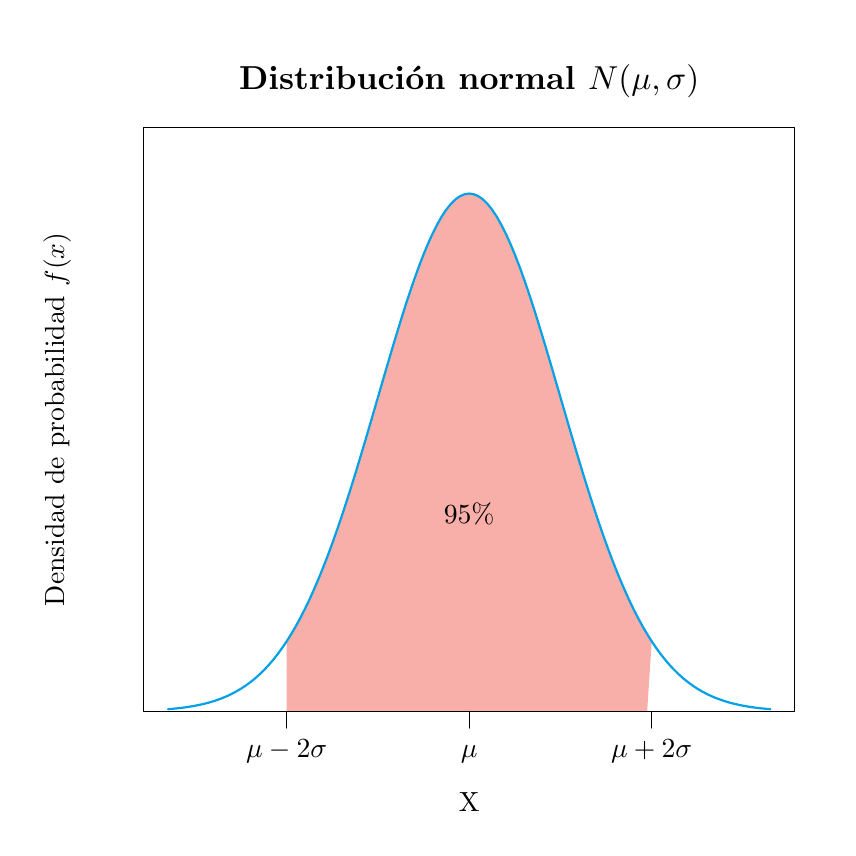
\begin{tikzpicture}[x=1pt,y=1pt]
\definecolor{fillColor}{RGB}{255,255,255}
\path[use as bounding box,fill=fillColor,fill opacity=0.00] (0,0) rectangle (289.08,289.08);
\begin{scope}
\path[clip] (  0.00,  0.00) rectangle (289.08,289.08);
\definecolor{drawColor}{RGB}{0,0,0}

\node[text=drawColor,anchor=base,inner sep=0pt, outer sep=0pt, scale=  1.20] at (159.54,266.89) {\bfseries Distribución normal $N(\mu,\sigma)$};

\node[text=drawColor,anchor=base,inner sep=0pt, outer sep=0pt, scale=  1.00] at (159.54,  6.00) {X};

\node[text=drawColor,rotate= 90.00,anchor=base,inner sep=0pt, outer sep=0pt, scale=  1.00] at ( 13.20,147.54) {Densidad de probabilidad $f(x)$};
\end{scope}
\begin{scope}
\path[clip] (  0.00,  0.00) rectangle (289.08,289.08);
\definecolor{drawColor}{RGB}{0,0,0}

\path[draw=drawColor,line width= 0.4pt,line join=round,line cap=round] (159.54, 42.00) -- (159.54, 42.00);

\path[draw=drawColor,line width= 0.4pt,line join=round,line cap=round] (159.54, 42.00) -- (159.54, 36.00);

\node[text=drawColor,anchor=base,inner sep=0pt, outer sep=0pt, scale=  1.00] at (159.54, 25.20) {$\mu$};

\path[draw=drawColor,line width= 0.4pt,line join=round,line cap=round] ( 93.58, 42.00) -- (225.50, 42.00);

\path[draw=drawColor,line width= 0.4pt,line join=round,line cap=round] ( 93.58, 42.00) -- ( 93.58, 36.00);

\path[draw=drawColor,line width= 0.4pt,line join=round,line cap=round] (225.50, 42.00) -- (225.50, 36.00);

\node[text=drawColor,anchor=base,inner sep=0pt, outer sep=0pt, scale=  1.00] at ( 93.58, 25.20) {$\mu-2\sigma$};

\node[text=drawColor,anchor=base,inner sep=0pt, outer sep=0pt, scale=  1.00] at (225.50, 25.20) {$\mu+2\sigma$};
\end{scope}
\begin{scope}
\path[clip] ( 42.00, 42.00) rectangle (277.08,253.08);
\definecolor{fillColor}{RGB}{238,50,36}

\path[fill=fillColor,fill opacity=0.39] ( 93.58, 42.00) --
	( 93.58, 67.33) --
	( 95.23, 69.95) --
	( 96.88, 72.78) --
	( 98.53, 75.80) --
	(100.18, 79.03) --
	(101.83, 82.47) --
	(103.47, 86.12) --
	(105.12, 89.97) --
	(106.77, 94.03) --
	(108.42, 98.29) --
	(110.07,102.75) --
	(111.72,107.40) --
	(113.37,112.23) --
	(115.02,117.23) --
	(116.67,122.38) --
	(118.32,127.67) --
	(119.96,133.09) --
	(121.61,138.60) --
	(123.26,144.19) --
	(124.91,149.83) --
	(126.56,155.50) --
	(128.21,161.17) --
	(129.86,166.81) --
	(131.51,172.39) --
	(133.16,177.88) --
	(134.81,183.25) --
	(136.45,188.47) --
	(138.10,193.50) --
	(139.75,198.30) --
	(141.40,202.86) --
	(143.05,207.14) --
	(144.70,211.11) --
	(146.35,214.74) --
	(148.00,218.01) --
	(149.65,220.90) --
	(151.30,223.37) --
	(152.94,225.43) --
	(154.59,227.04) --
	(156.24,228.20) --
	(157.89,228.90) --
	(159.54,229.13) --
	(161.19,228.90) --
	(162.84,228.20) --
	(164.49,227.04) --
	(166.14,225.43) --
	(167.78,223.37) --
	(169.43,220.90) --
	(171.08,218.01) --
	(172.73,214.74) --
	(174.38,211.11) --
	(176.03,207.14) --
	(177.68,202.86) --
	(179.33,198.30) --
	(180.98,193.50) --
	(182.63,188.47) --
	(184.27,183.25) --
	(185.92,177.88) --
	(187.57,172.39) --
	(189.22,166.81) --
	(190.87,161.17) --
	(192.52,155.50) --
	(194.17,149.83) --
	(195.82,144.19) --
	(197.47,138.60) --
	(199.12,133.09) --
	(200.76,127.67) --
	(202.41,122.38) --
	(204.06,117.23) --
	(205.71,112.23) --
	(207.36,107.40) --
	(209.01,102.75) --
	(210.66, 98.29) --
	(212.31, 94.03) --
	(213.96, 89.97) --
	(215.61, 86.12) --
	(217.25, 82.47) --
	(218.90, 79.03) --
	(220.55, 75.80) --
	(222.20, 72.78) --
	(223.85, 69.95) --
	(225.50, 67.33) --
	(223.85, 42.00) --
	cycle;
\definecolor{drawColor}{RGB}{0,0,0}

\node[text=drawColor,anchor=base,inner sep=0pt, outer sep=0pt, scale=  1.00] at (159.54,109.86) {$95\%$};
\definecolor{drawColor}{RGB}{5,161,230}

\path[draw=drawColor,line width= 0.8pt,line join=round,line cap=round] ( 50.71, 42.81) --
	( 52.36, 42.95) --
	( 54.00, 43.12) --
	( 55.65, 43.31) --
	( 57.30, 43.53) --
	( 58.95, 43.79) --
	( 60.60, 44.08) --
	( 62.25, 44.41) --
	( 63.90, 44.79) --
	( 65.55, 45.22) --
	( 67.20, 45.71) --
	( 68.85, 46.27) --
	( 70.49, 46.89) --
	( 72.14, 47.59) --
	( 73.79, 48.37) --
	( 75.44, 49.25) --
	( 77.09, 50.22) --
	( 78.74, 51.31) --
	( 80.39, 52.50) --
	( 82.04, 53.83) --
	( 83.69, 55.29) --
	( 85.34, 56.89) --
	( 86.98, 58.64) --
	( 88.63, 60.55) --
	( 90.28, 62.63) --
	( 91.93, 64.89) --
	( 93.58, 67.33) --
	( 95.23, 69.95) --
	( 96.88, 72.78) --
	( 98.53, 75.80) --
	(100.18, 79.03) --
	(101.83, 82.47) --
	(103.47, 86.12) --
	(105.12, 89.97) --
	(106.77, 94.03) --
	(108.42, 98.29) --
	(110.07,102.75) --
	(111.72,107.40) --
	(113.37,112.23) --
	(115.02,117.23) --
	(116.67,122.38) --
	(118.32,127.67) --
	(119.96,133.09) --
	(121.61,138.60) --
	(123.26,144.19) --
	(124.91,149.83) --
	(126.56,155.50) --
	(128.21,161.17) --
	(129.86,166.81) --
	(131.51,172.39) --
	(133.16,177.88) --
	(134.81,183.25) --
	(136.45,188.47) --
	(138.10,193.50) --
	(139.75,198.30) --
	(141.40,202.86) --
	(143.05,207.14) --
	(144.70,211.11) --
	(146.35,214.74) --
	(148.00,218.01) --
	(149.65,220.90) --
	(151.30,223.37) --
	(152.94,225.43) --
	(154.59,227.04) --
	(156.24,228.20) --
	(157.89,228.90) --
	(159.54,229.13) --
	(161.19,228.90) --
	(162.84,228.20) --
	(164.49,227.04) --
	(166.14,225.43) --
	(167.78,223.37) --
	(169.43,220.90) --
	(171.08,218.01) --
	(172.73,214.74) --
	(174.38,211.11) --
	(176.03,207.14) --
	(177.68,202.86) --
	(179.33,198.30) --
	(180.98,193.50) --
	(182.63,188.47) --
	(184.27,183.25) --
	(185.92,177.88) --
	(187.57,172.39) --
	(189.22,166.81) --
	(190.87,161.17) --
	(192.52,155.50) --
	(194.17,149.83) --
	(195.82,144.19) --
	(197.47,138.60) --
	(199.12,133.09) --
	(200.76,127.67) --
	(202.41,122.38) --
	(204.06,117.23) --
	(205.71,112.23) --
	(207.36,107.40) --
	(209.01,102.75) --
	(210.66, 98.29) --
	(212.31, 94.03) --
	(213.96, 89.97) --
	(215.61, 86.12) --
	(217.25, 82.47) --
	(218.90, 79.03) --
	(220.55, 75.80) --
	(222.20, 72.78) --
	(223.85, 69.95) --
	(225.50, 67.33) --
	(227.15, 64.89) --
	(228.80, 62.63) --
	(230.45, 60.55) --
	(232.10, 58.64) --
	(233.74, 56.89) --
	(235.39, 55.29) --
	(237.04, 53.83) --
	(238.69, 52.50) --
	(240.34, 51.31) --
	(241.99, 50.22) --
	(243.64, 49.25) --
	(245.29, 48.37) --
	(246.94, 47.59) --
	(248.59, 46.89) --
	(250.23, 46.27) --
	(251.88, 45.71) --
	(253.53, 45.22) --
	(255.18, 44.79) --
	(256.83, 44.41) --
	(258.48, 44.08) --
	(260.13, 43.79) --
	(261.78, 43.53) --
	(263.43, 43.31) --
	(265.08, 43.12) --
	(266.72, 42.95) --
	(268.37, 42.81);
\end{scope}
\begin{scope}
\path[clip] (  0.00,  0.00) rectangle (289.08,289.08);
\definecolor{drawColor}{RGB}{0,0,0}

\path[draw=drawColor,line width= 0.4pt,line join=round,line cap=round] ( 42.00, 42.00) --
	(277.08, 42.00) --
	(277.08,253.08) --
	( 42.00,253.08) --
	( 42.00, 42.00);
\end{scope}
\end{tikzpicture}

	\tikzsetnextfilename{variables_aleatorias_continuas/intervalo_normal_99}}
	\resizebox{0.33\textwidth}{!}{% Created by tikzDevice version 0.10.1 on 2016-05-10 09:59:46
% !TEX encoding = UTF-8 Unicode
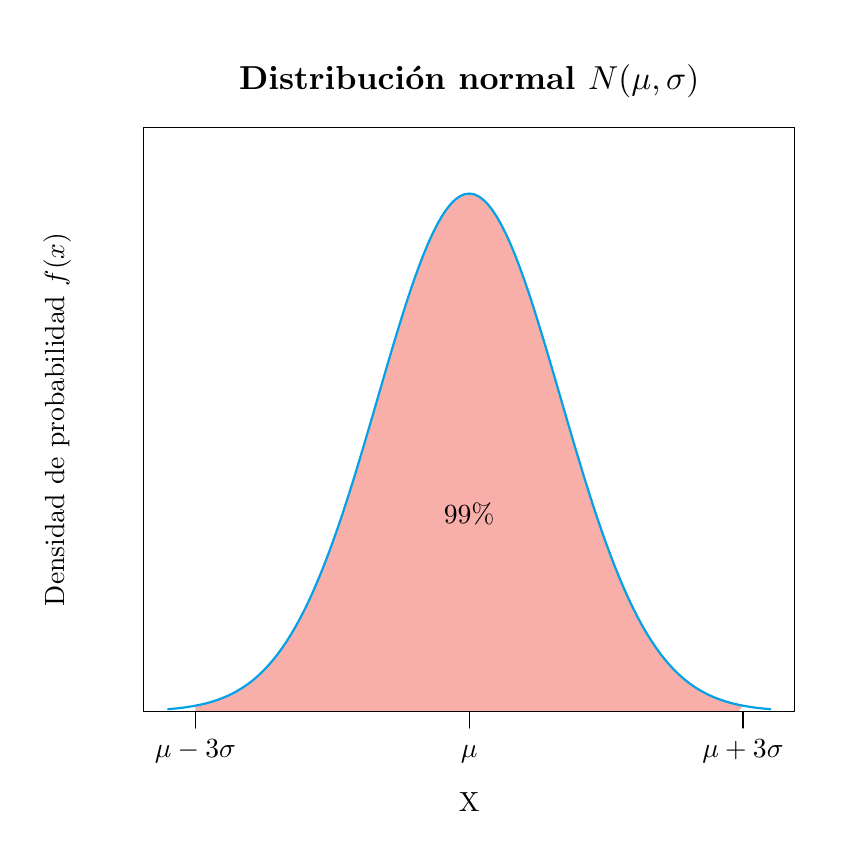
\begin{tikzpicture}[x=1pt,y=1pt]
\definecolor{fillColor}{RGB}{255,255,255}
\path[use as bounding box,fill=fillColor,fill opacity=0.00] (0,0) rectangle (289.08,289.08);
\begin{scope}
\path[clip] (  0.00,  0.00) rectangle (289.08,289.08);
\definecolor{drawColor}{RGB}{0,0,0}

\node[text=drawColor,anchor=base,inner sep=0pt, outer sep=0pt, scale=  1.20] at (159.54,266.89) {\bfseries Distribución normal $N(\mu,\sigma)$};

\node[text=drawColor,anchor=base,inner sep=0pt, outer sep=0pt, scale=  1.00] at (159.54,  6.00) {X};

\node[text=drawColor,rotate= 90.00,anchor=base,inner sep=0pt, outer sep=0pt, scale=  1.00] at ( 13.20,147.54) {Densidad de probabilidad $f(x)$};
\end{scope}
\begin{scope}
\path[clip] (  0.00,  0.00) rectangle (289.08,289.08);
\definecolor{drawColor}{RGB}{0,0,0}

\path[draw=drawColor,line width= 0.4pt,line join=round,line cap=round] (159.54, 42.00) -- (159.54, 42.00);

\path[draw=drawColor,line width= 0.4pt,line join=round,line cap=round] (159.54, 42.00) -- (159.54, 36.00);

\node[text=drawColor,anchor=base,inner sep=0pt, outer sep=0pt, scale=  1.00] at (159.54, 25.20) {$\mu$};

\path[draw=drawColor,line width= 0.4pt,line join=round,line cap=round] ( 60.60, 42.00) -- (258.48, 42.00);

\path[draw=drawColor,line width= 0.4pt,line join=round,line cap=round] ( 60.60, 42.00) -- ( 60.60, 36.00);

\path[draw=drawColor,line width= 0.4pt,line join=round,line cap=round] (258.48, 42.00) -- (258.48, 36.00);

\node[text=drawColor,anchor=base,inner sep=0pt, outer sep=0pt, scale=  1.00] at ( 60.60, 25.20) {$\mu-3\sigma$};

\node[text=drawColor,anchor=base,inner sep=0pt, outer sep=0pt, scale=  1.00] at (258.48, 25.20) {$\mu+3\sigma$};
\end{scope}
\begin{scope}
\path[clip] ( 42.00, 42.00) rectangle (277.08,253.08);
\definecolor{fillColor}{RGB}{238,50,36}

\path[fill=fillColor,fill opacity=0.39] ( 60.60, 42.00) --
	( 60.60, 44.08) --
	( 62.25, 44.41) --
	( 63.90, 44.79) --
	( 65.55, 45.22) --
	( 67.20, 45.71) --
	( 68.85, 46.27) --
	( 70.49, 46.89) --
	( 72.14, 47.59) --
	( 73.79, 48.37) --
	( 75.44, 49.25) --
	( 77.09, 50.22) --
	( 78.74, 51.31) --
	( 80.39, 52.50) --
	( 82.04, 53.83) --
	( 83.69, 55.29) --
	( 85.34, 56.89) --
	( 86.98, 58.64) --
	( 88.63, 60.55) --
	( 90.28, 62.63) --
	( 91.93, 64.89) --
	( 93.58, 67.33) --
	( 95.23, 69.95) --
	( 96.88, 72.78) --
	( 98.53, 75.80) --
	(100.18, 79.03) --
	(101.83, 82.47) --
	(103.47, 86.12) --
	(105.12, 89.97) --
	(106.77, 94.03) --
	(108.42, 98.29) --
	(110.07,102.75) --
	(111.72,107.40) --
	(113.37,112.23) --
	(115.02,117.23) --
	(116.67,122.38) --
	(118.32,127.67) --
	(119.96,133.09) --
	(121.61,138.60) --
	(123.26,144.19) --
	(124.91,149.83) --
	(126.56,155.50) --
	(128.21,161.17) --
	(129.86,166.81) --
	(131.51,172.39) --
	(133.16,177.88) --
	(134.81,183.25) --
	(136.45,188.47) --
	(138.10,193.50) --
	(139.75,198.30) --
	(141.40,202.86) --
	(143.05,207.14) --
	(144.70,211.11) --
	(146.35,214.74) --
	(148.00,218.01) --
	(149.65,220.90) --
	(151.30,223.37) --
	(152.94,225.43) --
	(154.59,227.04) --
	(156.24,228.20) --
	(157.89,228.90) --
	(159.54,229.13) --
	(161.19,228.90) --
	(162.84,228.20) --
	(164.49,227.04) --
	(166.14,225.43) --
	(167.78,223.37) --
	(169.43,220.90) --
	(171.08,218.01) --
	(172.73,214.74) --
	(174.38,211.11) --
	(176.03,207.14) --
	(177.68,202.86) --
	(179.33,198.30) --
	(180.98,193.50) --
	(182.63,188.47) --
	(184.27,183.25) --
	(185.92,177.88) --
	(187.57,172.39) --
	(189.22,166.81) --
	(190.87,161.17) --
	(192.52,155.50) --
	(194.17,149.83) --
	(195.82,144.19) --
	(197.47,138.60) --
	(199.12,133.09) --
	(200.76,127.67) --
	(202.41,122.38) --
	(204.06,117.23) --
	(205.71,112.23) --
	(207.36,107.40) --
	(209.01,102.75) --
	(210.66, 98.29) --
	(212.31, 94.03) --
	(213.96, 89.97) --
	(215.61, 86.12) --
	(217.25, 82.47) --
	(218.90, 79.03) --
	(220.55, 75.80) --
	(222.20, 72.78) --
	(223.85, 69.95) --
	(225.50, 67.33) --
	(227.15, 64.89) --
	(228.80, 62.63) --
	(230.45, 60.55) --
	(232.10, 58.64) --
	(233.74, 56.89) --
	(235.39, 55.29) --
	(237.04, 53.83) --
	(238.69, 52.50) --
	(240.34, 51.31) --
	(241.99, 50.22) --
	(243.64, 49.25) --
	(245.29, 48.37) --
	(246.94, 47.59) --
	(248.59, 46.89) --
	(250.23, 46.27) --
	(251.88, 45.71) --
	(253.53, 45.22) --
	(255.18, 44.79) --
	(256.83, 44.41) --
	(258.48, 44.08) --
	(256.83, 42.00) --
	cycle;
\definecolor{drawColor}{RGB}{0,0,0}

\node[text=drawColor,anchor=base,inner sep=0pt, outer sep=0pt, scale=  1.00] at (159.54,109.86) {$99\%$};
\definecolor{drawColor}{RGB}{5,161,230}

\path[draw=drawColor,line width= 0.8pt,line join=round,line cap=round] ( 50.71, 42.81) --
	( 52.36, 42.95) --
	( 54.00, 43.12) --
	( 55.65, 43.31) --
	( 57.30, 43.53) --
	( 58.95, 43.79) --
	( 60.60, 44.08) --
	( 62.25, 44.41) --
	( 63.90, 44.79) --
	( 65.55, 45.22) --
	( 67.20, 45.71) --
	( 68.85, 46.27) --
	( 70.49, 46.89) --
	( 72.14, 47.59) --
	( 73.79, 48.37) --
	( 75.44, 49.25) --
	( 77.09, 50.22) --
	( 78.74, 51.31) --
	( 80.39, 52.50) --
	( 82.04, 53.83) --
	( 83.69, 55.29) --
	( 85.34, 56.89) --
	( 86.98, 58.64) --
	( 88.63, 60.55) --
	( 90.28, 62.63) --
	( 91.93, 64.89) --
	( 93.58, 67.33) --
	( 95.23, 69.95) --
	( 96.88, 72.78) --
	( 98.53, 75.80) --
	(100.18, 79.03) --
	(101.83, 82.47) --
	(103.47, 86.12) --
	(105.12, 89.97) --
	(106.77, 94.03) --
	(108.42, 98.29) --
	(110.07,102.75) --
	(111.72,107.40) --
	(113.37,112.23) --
	(115.02,117.23) --
	(116.67,122.38) --
	(118.32,127.67) --
	(119.96,133.09) --
	(121.61,138.60) --
	(123.26,144.19) --
	(124.91,149.83) --
	(126.56,155.50) --
	(128.21,161.17) --
	(129.86,166.81) --
	(131.51,172.39) --
	(133.16,177.88) --
	(134.81,183.25) --
	(136.45,188.47) --
	(138.10,193.50) --
	(139.75,198.30) --
	(141.40,202.86) --
	(143.05,207.14) --
	(144.70,211.11) --
	(146.35,214.74) --
	(148.00,218.01) --
	(149.65,220.90) --
	(151.30,223.37) --
	(152.94,225.43) --
	(154.59,227.04) --
	(156.24,228.20) --
	(157.89,228.90) --
	(159.54,229.13) --
	(161.19,228.90) --
	(162.84,228.20) --
	(164.49,227.04) --
	(166.14,225.43) --
	(167.78,223.37) --
	(169.43,220.90) --
	(171.08,218.01) --
	(172.73,214.74) --
	(174.38,211.11) --
	(176.03,207.14) --
	(177.68,202.86) --
	(179.33,198.30) --
	(180.98,193.50) --
	(182.63,188.47) --
	(184.27,183.25) --
	(185.92,177.88) --
	(187.57,172.39) --
	(189.22,166.81) --
	(190.87,161.17) --
	(192.52,155.50) --
	(194.17,149.83) --
	(195.82,144.19) --
	(197.47,138.60) --
	(199.12,133.09) --
	(200.76,127.67) --
	(202.41,122.38) --
	(204.06,117.23) --
	(205.71,112.23) --
	(207.36,107.40) --
	(209.01,102.75) --
	(210.66, 98.29) --
	(212.31, 94.03) --
	(213.96, 89.97) --
	(215.61, 86.12) --
	(217.25, 82.47) --
	(218.90, 79.03) --
	(220.55, 75.80) --
	(222.20, 72.78) --
	(223.85, 69.95) --
	(225.50, 67.33) --
	(227.15, 64.89) --
	(228.80, 62.63) --
	(230.45, 60.55) --
	(232.10, 58.64) --
	(233.74, 56.89) --
	(235.39, 55.29) --
	(237.04, 53.83) --
	(238.69, 52.50) --
	(240.34, 51.31) --
	(241.99, 50.22) --
	(243.64, 49.25) --
	(245.29, 48.37) --
	(246.94, 47.59) --
	(248.59, 46.89) --
	(250.23, 46.27) --
	(251.88, 45.71) --
	(253.53, 45.22) --
	(255.18, 44.79) --
	(256.83, 44.41) --
	(258.48, 44.08) --
	(260.13, 43.79) --
	(261.78, 43.53) --
	(263.43, 43.31) --
	(265.08, 43.12) --
	(266.72, 42.95) --
	(268.37, 42.81);
\end{scope}
\begin{scope}
\path[clip] (  0.00,  0.00) rectangle (289.08,289.08);
\definecolor{drawColor}{RGB}{0,0,0}

\path[draw=drawColor,line width= 0.4pt,line join=round,line cap=round] ( 42.00, 42.00) --
	(277.08, 42.00) --
	(277.08,253.08) --
	( 42.00,253.08) --
	( 42.00, 42.00);
\end{scope}
\end{tikzpicture}
}
	}
	\mode<presentation>{\resizebox{0.5\textwidth}{!}{% Created by tikzDevice version 0.10.1 on 2016-05-09 14:41:45
% !TEX encoding = UTF-8 Unicode
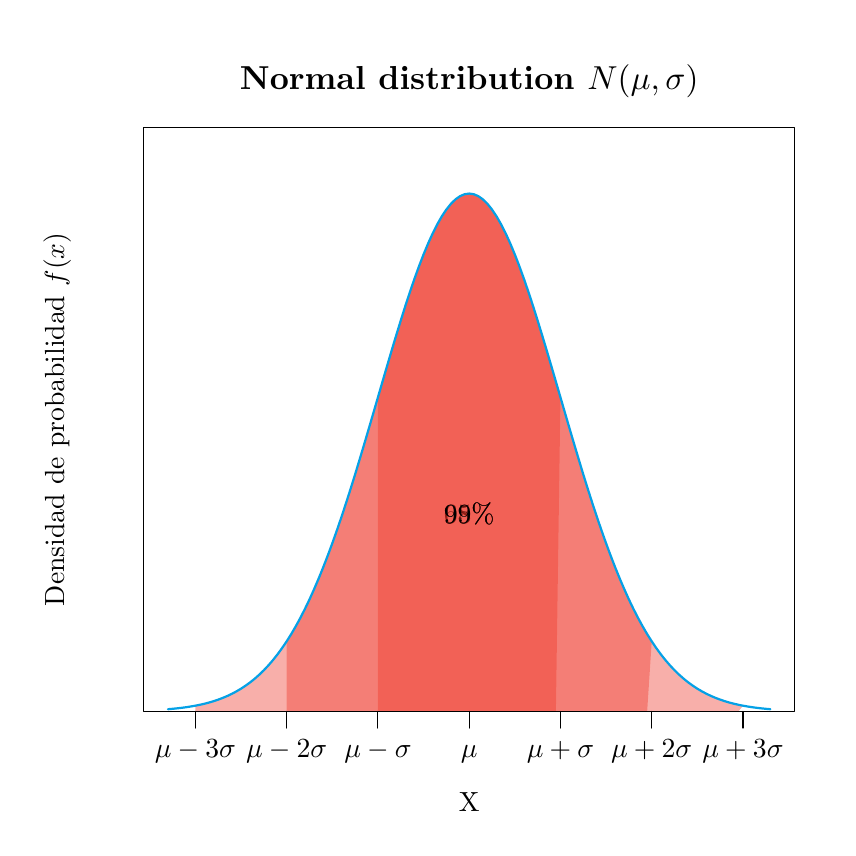
\begin{tikzpicture}[x=1pt,y=1pt]
\definecolor{fillColor}{RGB}{255,255,255}
\path[use as bounding box,fill=fillColor,fill opacity=0.00] (0,0) rectangle (289.08,289.08);
\begin{scope}
\path[clip] (  0.00,  0.00) rectangle (289.08,289.08);
\definecolor{drawColor}{RGB}{0,0,0}

\node[text=drawColor,anchor=base,inner sep=0pt, outer sep=0pt, scale=  1.20] at (159.54,266.89) {\bfseries Normal distribution $N(\mu,\sigma)$};

\node[text=drawColor,anchor=base,inner sep=0pt, outer sep=0pt, scale=  1.00] at (159.54,  6.00) {X};

\node[text=drawColor,rotate= 90.00,anchor=base,inner sep=0pt, outer sep=0pt, scale=  1.00] at ( 13.20,147.54) {Densidad de probabilidad $f(x)$};
\end{scope}
\begin{scope}
\path[clip] (  0.00,  0.00) rectangle (289.08,289.08);
\definecolor{drawColor}{RGB}{0,0,0}

\path[draw=drawColor,line width= 0.4pt,line join=round,line cap=round] (159.54, 42.00) -- (159.54, 42.00);

\path[draw=drawColor,line width= 0.4pt,line join=round,line cap=round] (159.54, 42.00) -- (159.54, 36.00);

\node[text=drawColor,anchor=base,inner sep=0pt, outer sep=0pt, scale=  1.00] at (159.54, 25.20) {$\mu$};

\path[draw=drawColor,line width= 0.4pt,line join=round,line cap=round] (126.56, 42.00) -- (192.52, 42.00);

\onslide<2>{\path[draw=drawColor,line width= 0.4pt,line join=round,line cap=round] (126.56, 42.00) -- (126.56, 36.00);

\path[draw=drawColor,line width= 0.4pt,line join=round,line cap=round] (192.52, 42.00) -- (192.52, 36.00);

\node[text=drawColor,anchor=base,inner sep=0pt, outer sep=0pt, scale=  1.00] at (126.56, 25.20) {$\mu-\sigma$};

\node[text=drawColor,anchor=base,inner sep=0pt, outer sep=0pt, scale=  1.00] at (192.52, 25.20) {$\mu+\sigma$};
}
\end{scope}

\onslide<2>{
\begin{scope}
\path[clip] ( 42.00, 42.00) rectangle (277.08,253.08);
\definecolor{fillColor}{RGB}{238,50,36}

\path[fill=fillColor,fill opacity=0.39] (126.56, 42.00) --
	(126.56,155.50) --
	(128.21,161.17) --
	(129.86,166.81) --
	(131.51,172.39) --
	(133.16,177.88) --
	(134.81,183.25) --
	(136.45,188.47) --
	(138.10,193.50) --
	(139.75,198.30) --
	(141.40,202.86) --
	(143.05,207.14) --
	(144.70,211.11) --
	(146.35,214.74) --
	(148.00,218.01) --
	(149.65,220.90) --
	(151.30,223.37) --
	(152.94,225.43) --
	(154.59,227.04) --
	(156.24,228.20) --
	(157.89,228.90) --
	(159.54,229.13) --
	(161.19,228.90) --
	(162.84,228.20) --
	(164.49,227.04) --
	(166.14,225.43) --
	(167.78,223.37) --
	(169.43,220.90) --
	(171.08,218.01) --
	(172.73,214.74) --
	(174.38,211.11) --
	(176.03,207.14) --
	(177.68,202.86) --
	(179.33,198.30) --
	(180.98,193.50) --
	(182.63,188.47) --
	(184.27,183.25) --
	(185.92,177.88) --
	(187.57,172.39) --
	(189.22,166.81) --
	(190.87,161.17) --
	(192.52,155.50) --
	(190.87, 42.00) --
	cycle;
\definecolor{drawColor}{RGB}{0,0,0}

\node[text=drawColor,anchor=base,inner sep=0pt, outer sep=0pt, scale=  1.00] at (159.54,109.86) {$68\%$};
\end{scope}
}
\onslide<3>{
\begin{scope}
\path[clip] (  0.00,  0.00) rectangle (289.08,289.08);
\definecolor{drawColor}{RGB}{0,0,0}

\path[draw=drawColor,line width= 0.4pt,line join=round,line cap=round] ( 93.58, 42.00) -- (225.50, 42.00);

\path[draw=drawColor,line width= 0.4pt,line join=round,line cap=round] ( 93.58, 42.00) -- ( 93.58, 36.00);

\path[draw=drawColor,line width= 0.4pt,line join=round,line cap=round] (225.50, 42.00) -- (225.50, 36.00);

\node[text=drawColor,anchor=base,inner sep=0pt, outer sep=0pt, scale=  1.00] at ( 93.58, 25.20) {$\mu-2\sigma$};

\node[text=drawColor,anchor=base,inner sep=0pt, outer sep=0pt, scale=  1.00] at (225.50, 25.20) {$\mu+2\sigma$};
\end{scope}
\begin{scope}
\path[clip] ( 42.00, 42.00) rectangle (277.08,253.08);
\definecolor{fillColor}{RGB}{238,50,36}

\path[fill=fillColor,fill opacity=0.39] ( 93.58, 42.00) --
	( 93.58, 67.33) --
	( 95.23, 69.95) --
	( 96.88, 72.78) --
	( 98.53, 75.80) --
	(100.18, 79.03) --
	(101.83, 82.47) --
	(103.47, 86.12) --
	(105.12, 89.97) --
	(106.77, 94.03) --
	(108.42, 98.29) --
	(110.07,102.75) --
	(111.72,107.40) --
	(113.37,112.23) --
	(115.02,117.23) --
	(116.67,122.38) --
	(118.32,127.67) --
	(119.96,133.09) --
	(121.61,138.60) --
	(123.26,144.19) --
	(124.91,149.83) --
	(126.56,155.50) --
	(128.21,161.17) --
	(129.86,166.81) --
	(131.51,172.39) --
	(133.16,177.88) --
	(134.81,183.25) --
	(136.45,188.47) --
	(138.10,193.50) --
	(139.75,198.30) --
	(141.40,202.86) --
	(143.05,207.14) --
	(144.70,211.11) --
	(146.35,214.74) --
	(148.00,218.01) --
	(149.65,220.90) --
	(151.30,223.37) --
	(152.94,225.43) --
	(154.59,227.04) --
	(156.24,228.20) --
	(157.89,228.90) --
	(159.54,229.13) --
	(161.19,228.90) --
	(162.84,228.20) --
	(164.49,227.04) --
	(166.14,225.43) --
	(167.78,223.37) --
	(169.43,220.90) --
	(171.08,218.01) --
	(172.73,214.74) --
	(174.38,211.11) --
	(176.03,207.14) --
	(177.68,202.86) --
	(179.33,198.30) --
	(180.98,193.50) --
	(182.63,188.47) --
	(184.27,183.25) --
	(185.92,177.88) --
	(187.57,172.39) --
	(189.22,166.81) --
	(190.87,161.17) --
	(192.52,155.50) --
	(194.17,149.83) --
	(195.82,144.19) --
	(197.47,138.60) --
	(199.12,133.09) --
	(200.76,127.67) --
	(202.41,122.38) --
	(204.06,117.23) --
	(205.71,112.23) --
	(207.36,107.40) --
	(209.01,102.75) --
	(210.66, 98.29) --
	(212.31, 94.03) --
	(213.96, 89.97) --
	(215.61, 86.12) --
	(217.25, 82.47) --
	(218.90, 79.03) --
	(220.55, 75.80) --
	(222.20, 72.78) --
	(223.85, 69.95) --
	(225.50, 67.33) --
	(223.85, 42.00) --
	cycle;
\definecolor{drawColor}{RGB}{0,0,0}

\node[text=drawColor,anchor=base,inner sep=0pt, outer sep=0pt, scale=  1.00] at (159.54,109.86) {$95\%$};
\end{scope}
}

\onslide<4>{
\begin{scope}
\path[clip] (  0.00,  0.00) rectangle (289.08,289.08);
\definecolor{drawColor}{RGB}{0,0,0}

\path[draw=drawColor,line width= 0.4pt,line join=round,line cap=round] ( 60.60, 42.00) -- (258.48, 42.00);

\path[draw=drawColor,line width= 0.4pt,line join=round,line cap=round] ( 60.60, 42.00) -- ( 60.60, 36.00);

\path[draw=drawColor,line width= 0.4pt,line join=round,line cap=round] (258.48, 42.00) -- (258.48, 36.00);

\node[text=drawColor,anchor=base,inner sep=0pt, outer sep=0pt, scale=  1.00] at ( 60.60, 25.20) {$\mu-3\sigma$};

\node[text=drawColor,anchor=base,inner sep=0pt, outer sep=0pt, scale=  1.00] at (258.48, 25.20) {$\mu+3\sigma$};
\end{scope}
}

\begin{scope}
\path[clip] ( 42.00, 42.00) rectangle (277.08,253.08);
\definecolor{fillColor}{RGB}{238,50,36}
\onslide<4>{
\path[fill=fillColor,fill opacity=0.39] ( 60.60, 42.00) --
	( 60.60, 44.08) --
	( 62.25, 44.41) --
	( 63.90, 44.79) --
	( 65.55, 45.22) --
	( 67.20, 45.71) --
	( 68.85, 46.27) --
	( 70.49, 46.89) --
	( 72.14, 47.59) --
	( 73.79, 48.37) --
	( 75.44, 49.25) --
	( 77.09, 50.22) --
	( 78.74, 51.31) --
	( 80.39, 52.50) --
	( 82.04, 53.83) --
	( 83.69, 55.29) --
	( 85.34, 56.89) --
	( 86.98, 58.64) --
	( 88.63, 60.55) --
	( 90.28, 62.63) --
	( 91.93, 64.89) --
	( 93.58, 67.33) --
	( 95.23, 69.95) --
	( 96.88, 72.78) --
	( 98.53, 75.80) --
	(100.18, 79.03) --
	(101.83, 82.47) --
	(103.47, 86.12) --
	(105.12, 89.97) --
	(106.77, 94.03) --
	(108.42, 98.29) --
	(110.07,102.75) --
	(111.72,107.40) --
	(113.37,112.23) --
	(115.02,117.23) --
	(116.67,122.38) --
	(118.32,127.67) --
	(119.96,133.09) --
	(121.61,138.60) --
	(123.26,144.19) --
	(124.91,149.83) --
	(126.56,155.50) --
	(128.21,161.17) --
	(129.86,166.81) --
	(131.51,172.39) --
	(133.16,177.88) --
	(134.81,183.25) --
	(136.45,188.47) --
	(138.10,193.50) --
	(139.75,198.30) --
	(141.40,202.86) --
	(143.05,207.14) --
	(144.70,211.11) --
	(146.35,214.74) --
	(148.00,218.01) --
	(149.65,220.90) --
	(151.30,223.37) --
	(152.94,225.43) --
	(154.59,227.04) --
	(156.24,228.20) --
	(157.89,228.90) --
	(159.54,229.13) --
	(161.19,228.90) --
	(162.84,228.20) --
	(164.49,227.04) --
	(166.14,225.43) --
	(167.78,223.37) --
	(169.43,220.90) --
	(171.08,218.01) --
	(172.73,214.74) --
	(174.38,211.11) --
	(176.03,207.14) --
	(177.68,202.86) --
	(179.33,198.30) --
	(180.98,193.50) --
	(182.63,188.47) --
	(184.27,183.25) --
	(185.92,177.88) --
	(187.57,172.39) --
	(189.22,166.81) --
	(190.87,161.17) --
	(192.52,155.50) --
	(194.17,149.83) --
	(195.82,144.19) --
	(197.47,138.60) --
	(199.12,133.09) --
	(200.76,127.67) --
	(202.41,122.38) --
	(204.06,117.23) --
	(205.71,112.23) --
	(207.36,107.40) --
	(209.01,102.75) --
	(210.66, 98.29) --
	(212.31, 94.03) --
	(213.96, 89.97) --
	(215.61, 86.12) --
	(217.25, 82.47) --
	(218.90, 79.03) --
	(220.55, 75.80) --
	(222.20, 72.78) --
	(223.85, 69.95) --
	(225.50, 67.33) --
	(227.15, 64.89) --
	(228.80, 62.63) --
	(230.45, 60.55) --
	(232.10, 58.64) --
	(233.74, 56.89) --
	(235.39, 55.29) --
	(237.04, 53.83) --
	(238.69, 52.50) --
	(240.34, 51.31) --
	(241.99, 50.22) --
	(243.64, 49.25) --
	(245.29, 48.37) --
	(246.94, 47.59) --
	(248.59, 46.89) --
	(250.23, 46.27) --
	(251.88, 45.71) --
	(253.53, 45.22) --
	(255.18, 44.79) --
	(256.83, 44.41) --
	(258.48, 44.08) --
	(256.83, 42.00) --
	cycle;
\definecolor{drawColor}{RGB}{0,0,0}

\node[text=drawColor,anchor=base,inner sep=0pt, outer sep=0pt, scale=  1.00] at (159.54,109.86) {$99\%$};
}

\definecolor{drawColor}{RGB}{5,161,230}

\path[draw=drawColor,line width= 0.8pt,line join=round,line cap=round] ( 50.71, 42.81) --
	( 52.36, 42.95) --
	( 54.00, 43.12) --
	( 55.65, 43.31) --
	( 57.30, 43.53) --
	( 58.95, 43.79) --
	( 60.60, 44.08) --
	( 62.25, 44.41) --
	( 63.90, 44.79) --
	( 65.55, 45.22) --
	( 67.20, 45.71) --
	( 68.85, 46.27) --
	( 70.49, 46.89) --
	( 72.14, 47.59) --
	( 73.79, 48.37) --
	( 75.44, 49.25) --
	( 77.09, 50.22) --
	( 78.74, 51.31) --
	( 80.39, 52.50) --
	( 82.04, 53.83) --
	( 83.69, 55.29) --
	( 85.34, 56.89) --
	( 86.98, 58.64) --
	( 88.63, 60.55) --
	( 90.28, 62.63) --
	( 91.93, 64.89) --
	( 93.58, 67.33) --
	( 95.23, 69.95) --
	( 96.88, 72.78) --
	( 98.53, 75.80) --
	(100.18, 79.03) --
	(101.83, 82.47) --
	(103.47, 86.12) --
	(105.12, 89.97) --
	(106.77, 94.03) --
	(108.42, 98.29) --
	(110.07,102.75) --
	(111.72,107.40) --
	(113.37,112.23) --
	(115.02,117.23) --
	(116.67,122.38) --
	(118.32,127.67) --
	(119.96,133.09) --
	(121.61,138.60) --
	(123.26,144.19) --
	(124.91,149.83) --
	(126.56,155.50) --
	(128.21,161.17) --
	(129.86,166.81) --
	(131.51,172.39) --
	(133.16,177.88) --
	(134.81,183.25) --
	(136.45,188.47) --
	(138.10,193.50) --
	(139.75,198.30) --
	(141.40,202.86) --
	(143.05,207.14) --
	(144.70,211.11) --
	(146.35,214.74) --
	(148.00,218.01) --
	(149.65,220.90) --
	(151.30,223.37) --
	(152.94,225.43) --
	(154.59,227.04) --
	(156.24,228.20) --
	(157.89,228.90) --
	(159.54,229.13) --
	(161.19,228.90) --
	(162.84,228.20) --
	(164.49,227.04) --
	(166.14,225.43) --
	(167.78,223.37) --
	(169.43,220.90) --
	(171.08,218.01) --
	(172.73,214.74) --
	(174.38,211.11) --
	(176.03,207.14) --
	(177.68,202.86) --
	(179.33,198.30) --
	(180.98,193.50) --
	(182.63,188.47) --
	(184.27,183.25) --
	(185.92,177.88) --
	(187.57,172.39) --
	(189.22,166.81) --
	(190.87,161.17) --
	(192.52,155.50) --
	(194.17,149.83) --
	(195.82,144.19) --
	(197.47,138.60) --
	(199.12,133.09) --
	(200.76,127.67) --
	(202.41,122.38) --
	(204.06,117.23) --
	(205.71,112.23) --
	(207.36,107.40) --
	(209.01,102.75) --
	(210.66, 98.29) --
	(212.31, 94.03) --
	(213.96, 89.97) --
	(215.61, 86.12) --
	(217.25, 82.47) --
	(218.90, 79.03) --
	(220.55, 75.80) --
	(222.20, 72.78) --
	(223.85, 69.95) --
	(225.50, 67.33) --
	(227.15, 64.89) --
	(228.80, 62.63) --
	(230.45, 60.55) --
	(232.10, 58.64) --
	(233.74, 56.89) --
	(235.39, 55.29) --
	(237.04, 53.83) --
	(238.69, 52.50) --
	(240.34, 51.31) --
	(241.99, 50.22) --
	(243.64, 49.25) --
	(245.29, 48.37) --
	(246.94, 47.59) --
	(248.59, 46.89) --
	(250.23, 46.27) --
	(251.88, 45.71) --
	(253.53, 45.22) --
	(255.18, 44.79) --
	(256.83, 44.41) --
	(258.48, 44.08) --
	(260.13, 43.79) --
	(261.78, 43.53) --
	(263.43, 43.31) --
	(265.08, 43.12) --
	(266.72, 42.95) --
	(268.37, 42.81);
\end{scope}
\begin{scope}
\path[clip] (  0.00,  0.00) rectangle (289.08,289.08);
\definecolor{drawColor}{RGB}{0,0,0}

\path[draw=drawColor,line width= 0.4pt,line join=round,line cap=round] ( 42.00, 42.00) --
	(277.08, 42.00) --
	(277.08,253.08) --
	( 42.00,253.08) --
	( 42.00, 42.00);
\end{scope}
\end{tikzpicture}
}}
\end{center}

\note{
Y también se cumple que
\begin{align*}
& P(\mu-\sigma \leq X \leq \mu+\sigma) = 0.68,\\
& P(\mu-2\sigma \leq X \leq \mu+2\sigma) = 0.95,\\
& P(\mu-3\sigma \leq X \leq \mu+3\sigma) = 0.99.
\end{align*}
}
\onslide<4->{es decir, casi la totalidad de los individuos de la población presentarán valores entre la media menos tres veces la desviación típica, y la
media mas tres veces la desviación típica.}
\end{frame}


%---------------------------------------------------------------------slide----
\begin{frame}
\frametitle{Propiedades de la distribución Normal}
\framesubtitle{Ejemplo}
En un estudio se ha comprobado que el nivel de colesterol total en mujeres
sanas de entre 40 y 50 años sigue una distribución normal de media de 210 mg/dl y desviación típica 20 mg/dl. 

Atendiendo a las propiedades de la campana de Gauss, se tiene que 
\begin{itemize}
\item El 68\% de las mujeres sanas tendrán el colesterol entre $210\pm 20$ mg/dl, es decir, entre 190 y 230 mg/dl.
\item El 95\% de las mujeres sanas tendrán el colesterol entre $210\pm 2\cdot 20$ mg/dl, es decir, entre 170 y 250 mg/dl.
\item El 99\% de las mujeres sanas tendrán el colesterol entre $210\pm 3\cdot 20$ mg/dl, es decir, entre 150 y 270 mg/dl.
\end{itemize}

\note{
Veamos una aplicación de estas propiedades. 

En un estudio se ha comprobado que el nivel de colesterol total en mujeres sanas de entre 40 y 50 años sigue una distribución normal de
media de 210 mg/dl y desviación típica 20 mg/dl. 
\emph{¿Qué quiere decir esto?}

Atendiendo a las propiedades de la campana de Gauss, se tiene que 
\begin{itemize}
\item El 68\% de las mujeres sanas tendrán el colesterol entre $210\pm 20$ mg/dl, es decir, entre 190 y 230 mg/dl.
\item El 95\% de las mujeres sanas tendrán el colesterol entre $210\pm 2\cdot 20$ mg/dl, es decir, entre 170 y 250
mg/dl.
\item El 99\% de las mujeres sanas tendrán el colesterol entre $210\pm 3\cdot 20$ mg/dl, es decir, entre 150 y 270
mg/dl.
\end{itemize}

En la analítica sanguínea suele utilizarse el intervalo $\mu\pm 2\sigma$ para detectar posibles patologías. En el caso
del coresterol, dicho intervalo es $[170\text{ mg/dl}, 250\text{ mg/dl}]$. Cuando una persona tiene el colesterol fuera
de estos límites, se tiende a pensar que tiene alguna patología, aunque ciertamente podría estar sana, pero la
probabilidad de que eso ocurra es sólo de un 5\%.
}
\end{frame}


%---------------------------------------------------------------------slide----
\begin{frame}
\frametitle{Propiedades de la distribución Normal}
\framesubtitle{Example blood analysis}
\begin{columns}
\begin{column}{0.47\textwidth}
	En la analítica sanguínea suele utilizarse el intervalo $\mu\pm 2\sigma$ para detectar posibles patologías. 
	En el caso del colesterol, dicho intervalo es $[170\text{ mg/dl}, 250\text{ mg/dl}]$. 
	
	Cuando una persona tiene el colesterol fuera	de estos límites, se tiende a pensar que tiene alguna patología, aunque ciertamente podría estar sana,pero la	probabilidad de que eso ocurra es sólo de un 5\%.
\end{column}
\begin{column}{0.47\textwidth}
\begin{center}
	\mode<article>{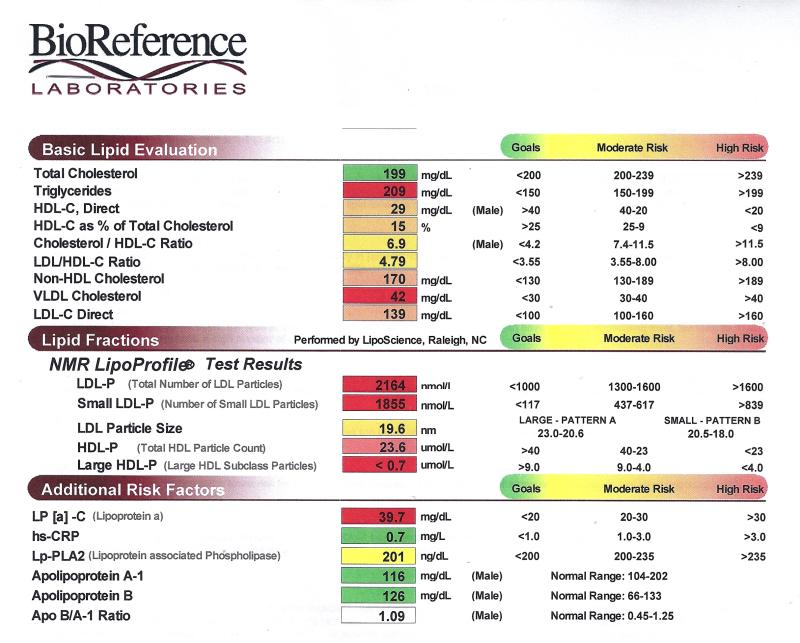
\includegraphics[width=0.7\textwidth]{img/variables_aleatorias_continuas/analitica_sanguinea.jpg}}
	\mode<presentation>{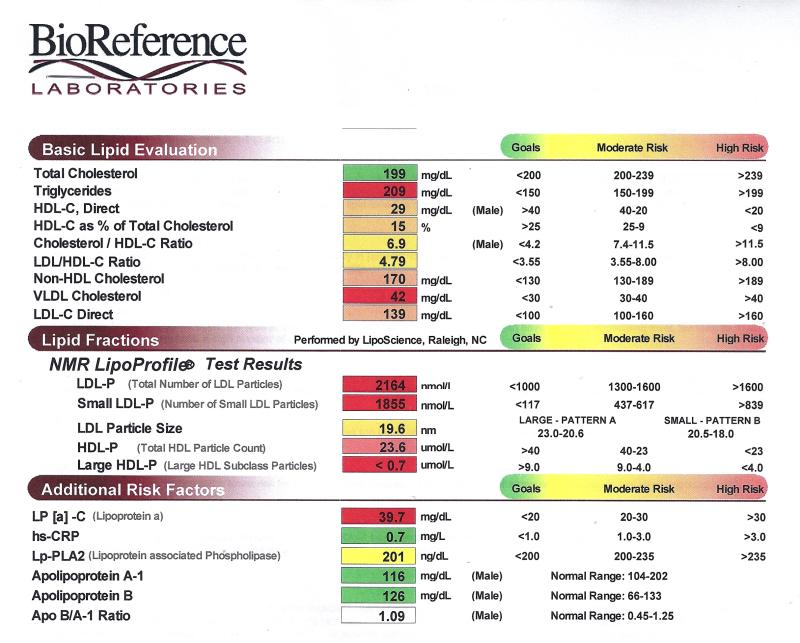
\includegraphics[width=\textwidth]{img/variables_aleatorias_continuas/analitica_sanguinea.jpg}}
\end{center}
\end{column}
\end{columns}
\end{frame}
	

%---------------------------------------------------------------------slide----
\begin{frame}
\frametitle{El teorema central del límite}
El comportamiento anterior lo presentan muchas variables continuas físicas y biológicas.

Si se piensa por ejemplo en la distribución de las estaturas, se verá que la mayor parte de los individuos presentan estaturas en torno a la
media, tanto por arriba, como por debajo, pero que a medida que van alejándose de la media, cada vez hay menos individuos con dichas
estaturas.

La justificación de que la distribución normal aparezca de manera tan frecuente en la naturaleza la encontramos en el
\highlight{\textbf{teorema central del límite}}, que veremos más adelante, y que establece que si una variable aleatoria continua proviene de un
experimento aleatorio cuyos resultados son debidos a un conjunto muy grande de factores independientes que actúan sumando sus efectos, entonces sigue una distribución aproximadamente normal.

\note{
Se ha observado que la mayor parte de las variables continuas físicas y biológicas presentan una distribucón con forma de campana de Gauss.

Si se piensa por ejemplo en la distribución de las estaturas, se verá que la mayor parte de los individuos presentan estaturas en torno a la
media, tanto por arriba, como por debajo, pero que a medida que van alejándose de la media, cada vez hay menos individuos con dichas
estaturas.

La justificación de que la distribución normal aparezca de manera tan frecuente en la naturaleza la encontramos en el
\structure{\textbf{teorema central del límite}}, que veremos más detenidamente en el siguiente tema, y que establece que si una variable
aleatoria $X$ proviene de un experimento aleatorio cuyos resultados son debidos a un conjunto muy grande de causas independientes que actúan
sumando sus efectos, entonces $X$ sigue una distribución aproximadamente normal.

Si pensamos en cualquier variable biológica, como por ejemplo la tensión arterial, rápidamente podremos identificar multitud de factores que
influyen en ella, como por ejemplo la edad, el sexo, la dieta, el ejercicio físico, si se fuma o no, etc. El valor de la tensión arterial en
un individuo es el resultado de todos estos factores que suman sus efectos de manera independiente, y por ello, el el colesterol acaba
teniendo una distribución normal.
}
\end{frame}


%---------------------------------------------------------------------slide----
\begin{frame}
\frametitle{La distribución Normal estándar $N(0,1)$}
De todas las distribuciones normales, la más importante es la que tiene media $\mu=0$ y desviación típica $\sigma=1$, que se conoce como \highlight{\textbf{normal estándar}} y se designa por $Z\sim N(0,1)$.

\begin{center}
	\tikzsetnextfilename{variables_aleatorias_continuas/funcion_densidad_normal_estandar}
	\mode<article>{\resizebox{0.6\textwidth}{!}{%% Input file name: funcion_densidad_normal_estandar.fig
%% FIG version: 3.2
%% Orientation: Landscape
%% Justification: Flush Left
%% Units: Inches
%% Paper size: A4
%% Magnification: 100.0
%% Resolution: 1200ppi
%% Include the following in the preamble:
%% \usepackage{textcomp}
%% End

\begin{pspicture}(6.69cm,3.44cm)(16.66cm,13.45cm)
\psset{unit=0.8cm}
%%
%% Depth: 2147483647
%%
\newgray{mycolor0}{0.74}\definecolor{mycolor0}{gray}{0.74}
\newrgbcolor{mycolor1}{1.00 0.50 0.31}\definecolor{mycolor1}{rgb}{1.00,0.50,0.31}
%%
%% Depth: 100
%%
\psset{linestyle=solid,linewidth=0.03175,linecolor=mycolor1,fillstyle=none}
\psline(10.61,6.75)(10.70,6.76)(10.80,6.77)(10.89,6.79)(10.99,6.80)(11.08,6.82)(11.17,6.84)(11.27,6.87)(11.36,6.90)(11.46,6.94)(11.55,6.98)(11.64,7.03)(11.74,7.08)(11.83,7.15)(11.93,7.22)(12.02,7.31)(12.12,7.40)(12.21,7.51)(12.30,7.63)(12.40,7.77)(12.49,7.92)(12.59,8.08)(12.68,8.26)(12.78,8.45)(12.87,8.67)(12.96,8.89)(13.06,9.14)(13.15,9.40)(13.25,9.67)(13.34,9.95)(13.43,10.26)(13.53,10.56)(13.62,10.88)(13.72,11.21)(13.81,11.54)(13.91,11.87)(14.00,12.20)(14.09,12.52)(14.19,12.84)(14.28,13.14)(14.38,13.43)(14.47,13.70)(14.56,13.96)(14.66,14.18)(14.76,14.38)(14.85,14.55)(14.94,14.69)(15.04,14.80)(15.13,14.87)(15.23,14.91)(15.32,14.91)(15.41,14.87)(15.51,14.80)(15.60,14.69)(15.70,14.55)(15.79,14.38)(15.89,14.18)(15.98,13.96)(16.07,13.70)(16.17,13.43)(16.26,13.14)(16.36,12.84)(16.45,12.52)(16.54,12.20)(16.64,11.87)(16.73,11.54)(16.83,11.21)(16.92,10.88)(17.02,10.56)(17.11,10.26)(17.20,9.95)(17.30,9.67)(17.39,9.40)(17.49,9.14)(17.58,8.89)(17.68,8.67)(17.77,8.45)(17.86,8.26)(17.96,8.08)(18.05,7.92)(18.15,7.77)(18.24,7.63)(18.33,7.51)(18.43,7.40)(18.52,7.31)(18.62,7.22)(18.71,7.15)(18.81,7.08)(18.90,7.03)(18.99,6.98)(19.09,6.94)(19.18,6.90)(19.28,6.87)(19.37,6.84)(19.47,6.82)(19.56,6.80)(19.66,6.79)(19.75,6.77)(19.84,6.76)(19.94,6.75)
\psset{linecolor=black}
\psline(11.02,6.43)(19.52,6.43)
\psline(11.02,6.43)(11.02,6.22)
\psline(12.44,6.43)(12.44,6.22)
\psline(13.86,6.43)(13.86,6.22)
\psline(15.27,6.43)(15.27,6.22)
\psline(16.69,6.43)(16.69,6.22)
\psline(18.11,6.43)(18.11,6.22)
\psline(19.52,6.43)(19.52,6.22)
\rput(11.02,5.67){-3}
\rput(12.44,5.67){-2}
\rput(13.86,5.67){-1}
\rput(15.27,5.67){0}
\rput(16.69,5.67){1}
\rput(18.11,5.67){2}
\rput(19.52,5.67){3}
\psline(10.23,6.72)(10.23,14.94)
\psline(10.23,6.72)(10.02,6.72)
\psline(10.23,8.77)(10.02,8.77)
\psline(10.23,10.83)(10.02,10.83)
\psline(10.23,12.88)(10.02,12.88)
\psline(10.23,14.94)(10.02,14.94)
\rput{90}(9.73,6.72){0.0}
\rput{90}(9.73,8.77){0.1}
\rput{90}(9.73,10.83){0.2}
\rput{90}(9.73,12.88){0.3}
\rput{90}(9.73,14.94){0.4}
\psline(10.23,6.43)(20.31,6.43)(20.31,15.23)(10.23,15.23)(10.23,6.43)
\rput[l](11.14,15.99){Distribución normal estándar $N(\mu=0,\sigma=1)$}
\rput(15.27,4.82){$Z$}
\rput[l]{90}(8.88,8.46){Densidad de probabilidad $f(z)$}
\psset{linecolor=mycolor0}
\psline(10.23,6.72)(20.31,6.72)
\end{pspicture}
%% End
}}
	\mode<presentation>{\resizebox{0.55\textwidth}{!}{%% Input file name: funcion_densidad_normal_estandar.fig
%% FIG version: 3.2
%% Orientation: Landscape
%% Justification: Flush Left
%% Units: Inches
%% Paper size: A4
%% Magnification: 100.0
%% Resolution: 1200ppi
%% Include the following in the preamble:
%% \usepackage{textcomp}
%% End

\begin{pspicture}(6.69cm,3.44cm)(16.66cm,13.45cm)
\psset{unit=0.8cm}
%%
%% Depth: 2147483647
%%
\newgray{mycolor0}{0.74}\definecolor{mycolor0}{gray}{0.74}
\newrgbcolor{mycolor1}{1.00 0.50 0.31}\definecolor{mycolor1}{rgb}{1.00,0.50,0.31}
%%
%% Depth: 100
%%
\psset{linestyle=solid,linewidth=0.03175,linecolor=mycolor1,fillstyle=none}
\psline(10.61,6.75)(10.70,6.76)(10.80,6.77)(10.89,6.79)(10.99,6.80)(11.08,6.82)(11.17,6.84)(11.27,6.87)(11.36,6.90)(11.46,6.94)(11.55,6.98)(11.64,7.03)(11.74,7.08)(11.83,7.15)(11.93,7.22)(12.02,7.31)(12.12,7.40)(12.21,7.51)(12.30,7.63)(12.40,7.77)(12.49,7.92)(12.59,8.08)(12.68,8.26)(12.78,8.45)(12.87,8.67)(12.96,8.89)(13.06,9.14)(13.15,9.40)(13.25,9.67)(13.34,9.95)(13.43,10.26)(13.53,10.56)(13.62,10.88)(13.72,11.21)(13.81,11.54)(13.91,11.87)(14.00,12.20)(14.09,12.52)(14.19,12.84)(14.28,13.14)(14.38,13.43)(14.47,13.70)(14.56,13.96)(14.66,14.18)(14.76,14.38)(14.85,14.55)(14.94,14.69)(15.04,14.80)(15.13,14.87)(15.23,14.91)(15.32,14.91)(15.41,14.87)(15.51,14.80)(15.60,14.69)(15.70,14.55)(15.79,14.38)(15.89,14.18)(15.98,13.96)(16.07,13.70)(16.17,13.43)(16.26,13.14)(16.36,12.84)(16.45,12.52)(16.54,12.20)(16.64,11.87)(16.73,11.54)(16.83,11.21)(16.92,10.88)(17.02,10.56)(17.11,10.26)(17.20,9.95)(17.30,9.67)(17.39,9.40)(17.49,9.14)(17.58,8.89)(17.68,8.67)(17.77,8.45)(17.86,8.26)(17.96,8.08)(18.05,7.92)(18.15,7.77)(18.24,7.63)(18.33,7.51)(18.43,7.40)(18.52,7.31)(18.62,7.22)(18.71,7.15)(18.81,7.08)(18.90,7.03)(18.99,6.98)(19.09,6.94)(19.18,6.90)(19.28,6.87)(19.37,6.84)(19.47,6.82)(19.56,6.80)(19.66,6.79)(19.75,6.77)(19.84,6.76)(19.94,6.75)
\psset{linecolor=black}
\psline(11.02,6.43)(19.52,6.43)
\psline(11.02,6.43)(11.02,6.22)
\psline(12.44,6.43)(12.44,6.22)
\psline(13.86,6.43)(13.86,6.22)
\psline(15.27,6.43)(15.27,6.22)
\psline(16.69,6.43)(16.69,6.22)
\psline(18.11,6.43)(18.11,6.22)
\psline(19.52,6.43)(19.52,6.22)
\rput(11.02,5.67){-3}
\rput(12.44,5.67){-2}
\rput(13.86,5.67){-1}
\rput(15.27,5.67){0}
\rput(16.69,5.67){1}
\rput(18.11,5.67){2}
\rput(19.52,5.67){3}
\psline(10.23,6.72)(10.23,14.94)
\psline(10.23,6.72)(10.02,6.72)
\psline(10.23,8.77)(10.02,8.77)
\psline(10.23,10.83)(10.02,10.83)
\psline(10.23,12.88)(10.02,12.88)
\psline(10.23,14.94)(10.02,14.94)
\rput{90}(9.73,6.72){0.0}
\rput{90}(9.73,8.77){0.1}
\rput{90}(9.73,10.83){0.2}
\rput{90}(9.73,12.88){0.3}
\rput{90}(9.73,14.94){0.4}
\psline(10.23,6.43)(20.31,6.43)(20.31,15.23)(10.23,15.23)(10.23,6.43)
\rput[l](11.14,15.99){Distribución normal estándar $N(\mu=0,\sigma=1)$}
\rput(15.27,4.82){$Z$}
\rput[l]{90}(8.88,8.46){Densidad de probabilidad $f(z)$}
\psset{linecolor=mycolor0}
\psline(10.23,6.72)(20.31,6.72)
\end{pspicture}
%% End
}}
\end{center}

\note{
De todas las distribuciones normales, la más importante es la que tiene media $\mu=0$ y desviación típica $\sigma=1$,
que se conoce como \highlight{\textbf{normal estándar}} y se designa por $Z$.

Su función de densidad será una campana de Gauss centrada en el 0, en la que el 99\% de los individuos estarán entre -3 y 3. 
}
\end{frame}


%---------------------------------------------------------------------slide----
\begin{frame}
\frametitle{Cálculo de probabilidades con la Normal estándar}
\framesubtitle{Manejo de la tabla de la función de distribución}
Para evitar tener que calcular probabilidades integrando la función de densidad de la normal estándar es habitual utilizar su función de
distribución, que se da en forma de tabla como la siguiente.

\begin{columns}
\begin{column}{0.47\textwidth}
\begin{center}
	Por ejemplo, para calcular $P(Z\leq 0.52)$
	
	\mode<article>{\begin{tabular}[b]
{|r||r|r|r|r|}
\hline
\multicolumn{1}{|c||}{$\mathbf{z}$}& 
\multicolumn{1}{c|}{\textbf{0,00}}& 
\multicolumn{1}{c|}{\textbf{0,01}}& 
\multicolumn{1}{c|}{\alert{\textbf{0,02}}}& 
\multicolumn{1}{c|}{\textbf{\cdots}}\\
\hline\hline
\textbf{0,0}& 
0,5000& 
0,5040& 
0,5080& 
\cdots\\
\hline
\textbf{0,1}& 
0,5398& 
0,5438& 
0,5478& 
\cdots \\
\hline
\textbf{0,2}& 
0,5793& 
0,5832& 
0,5871& 
\cdots\\
\hline
\textbf{0,3}& 
0,6179& 
0,6217& 
0,6255& 
\cdots\\
\hline
\textbf{0,4}& 
0,6554& 
0,6591& 
0,6628& 
\cdots\\
\hline
\alert{\textbf{0,5}}& 
0,6915& 
0,6950& 
\cellcolor{coral}{\alert{\textbf{0,6985}}}& 
\cdots\\
\hline
\textbf{\vdots}& 
\vdots& 
\vdots& 
\vdots& 
\ddots\\
\hline
\end{tabular}}
	\mode<presentation>{\scalebox{0.9}{\begin{tabular}[b]
{|r||r|r|r|r|}
\hline
\multicolumn{1}{|c||}{$\mathbf{z}$}& 
\multicolumn{1}{c|}{\textbf{0,00}}& 
\multicolumn{1}{c|}{\textbf{0,01}}& 
\multicolumn{1}{c|}{\alert{\textbf{0,02}}}& 
\multicolumn{1}{c|}{\textbf{\cdots}}\\
\hline\hline
\textbf{0,0}& 
0,5000& 
0,5040& 
0,5080& 
\cdots\\
\hline
\textbf{0,1}& 
0,5398& 
0,5438& 
0,5478& 
\cdots \\
\hline
\textbf{0,2}& 
0,5793& 
0,5832& 
0,5871& 
\cdots\\
\hline
\textbf{0,3}& 
0,6179& 
0,6217& 
0,6255& 
\cdots\\
\hline
\textbf{0,4}& 
0,6554& 
0,6591& 
0,6628& 
\cdots\\
\hline
\alert{\textbf{0,5}}& 
0,6915& 
0,6950& 
\cellcolor{coral}{\alert{\textbf{0,6985}}}& 
\cdots\\
\hline
\textbf{\vdots}& 
\vdots& 
\vdots& 
\vdots& 
\ddots\\
\hline
\end{tabular}}}
	
	$0.52 \rightarrow $ fila $0.5$ + columna $0.02$
\end{center}
\end{column}
\begin{column}{0.53\textwidth}
\begin{center}
	\tikzsetnextfilename{variables_aleatorias_continuas/calculo_probabilidades_normal_cola_izquierda}
	\mode<article>{\resizebox{0.6\textwidth}{!}{% Created by tikzDevice version 0.10.1 on 2016-05-16 22:15:16
% !TEX encoding = UTF-8 Unicode
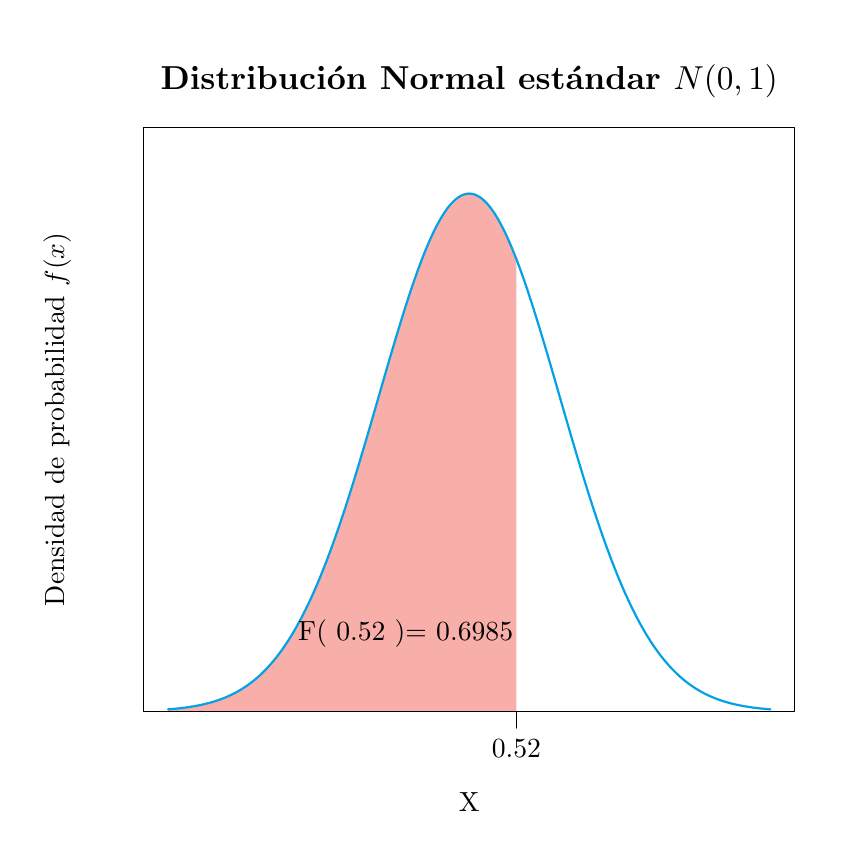
\begin{tikzpicture}[x=1pt,y=1pt]
\definecolor{fillColor}{RGB}{255,255,255}
\path[use as bounding box,fill=fillColor,fill opacity=0.00] (0,0) rectangle (289.08,289.08);
\begin{scope}
\path[clip] (  0.00,  0.00) rectangle (289.08,289.08);
\definecolor{drawColor}{RGB}{0,0,0}

\node[text=drawColor,anchor=base,inner sep=0pt, outer sep=0pt, scale=  1.20] at (159.54,266.89) {\bfseries Distribución Normal estándar $N(0,1)$};

\node[text=drawColor,anchor=base,inner sep=0pt, outer sep=0pt, scale=  1.00] at (159.54,  6.00) {X};

\node[text=drawColor,rotate= 90.00,anchor=base,inner sep=0pt, outer sep=0pt, scale=  1.00] at ( 13.20,147.54) {Densidad de probabilidad $f(x)$};
\end{scope}
\begin{scope}
\path[clip] (  0.00,  0.00) rectangle (289.08,289.08);
\definecolor{drawColor}{RGB}{0,0,0}

\path[draw=drawColor,line width= 0.4pt,line join=round,line cap=round] (176.59, 42.00) -- (176.59, 42.00);

\path[draw=drawColor,line width= 0.4pt,line join=round,line cap=round] (176.59, 42.00) -- (176.59, 36.00);

\node[text=drawColor,anchor=base,inner sep=0pt, outer sep=0pt, scale=  1.00] at (176.59, 25.20) {0.52};
\end{scope}
\begin{scope}
\path[clip] ( 42.00, 42.00) rectangle (277.08,253.08);
\definecolor{fillColor}{RGB}{238,50,36}

\path[fill=fillColor,fill opacity=0.39] ( 50.71, 42.00) --
	( 50.71, 42.76) --
	( 52.02, 42.86) --
	( 53.33, 42.98) --
	( 54.64, 43.12) --
	( 55.95, 43.27) --
	( 57.26, 43.44) --
	( 58.57, 43.63) --
	( 59.89, 43.84) --
	( 61.20, 44.08) --
	( 62.51, 44.34) --
	( 63.82, 44.63) --
	( 65.13, 44.96) --
	( 66.44, 45.32) --
	( 67.75, 45.71) --
	( 69.06, 46.15) --
	( 70.38, 46.63) --
	( 71.69, 47.16) --
	( 73.00, 47.74) --
	( 74.31, 48.37) --
	( 75.62, 49.06) --
	( 76.93, 49.82) --
	( 78.24, 50.64) --
	( 79.55, 51.54) --
	( 80.87, 52.50) --
	( 82.18, 53.55) --
	( 83.49, 54.69) --
	( 84.80, 55.91) --
	( 86.11, 57.23) --
	( 87.42, 58.64) --
	( 88.73, 60.16) --
	( 90.04, 61.78) --
	( 91.36, 63.51) --
	( 92.67, 65.36) --
	( 93.98, 67.33) --
	( 95.29, 69.41) --
	( 96.60, 71.62) --
	( 97.91, 73.96) --
	( 99.22, 76.43) --
	(100.53, 79.03) --
	(101.85, 81.77) --
	(103.16, 84.63) --
	(104.47, 87.63) --
	(105.78, 90.76) --
	(107.09, 94.03) --
	(108.40, 97.42) --
	(109.71,100.95) --
	(111.02,104.59) --
	(112.34,108.35) --
	(113.65,112.23) --
	(114.96,116.22) --
	(116.27,120.30) --
	(117.58,124.48) --
	(118.89,128.75) --
	(120.20,133.09) --
	(121.51,137.49) --
	(122.83,141.94) --
	(124.14,146.44) --
	(125.45,150.96) --
	(126.76,155.50) --
	(128.07,160.04) --
	(129.38,164.56) --
	(130.69,169.05) --
	(132.00,173.50) --
	(133.32,177.88) --
	(134.63,182.19) --
	(135.94,186.40) --
	(137.25,190.50) --
	(138.56,194.48) --
	(139.87,198.30) --
	(141.18,201.97) --
	(142.49,205.47) --
	(143.81,208.77) --
	(145.12,211.87) --
	(146.43,214.74) --
	(147.74,217.39) --
	(149.05,219.79) --
	(150.36,221.94) --
	(151.67,223.82) --
	(152.98,225.43) --
	(154.30,226.75) --
	(155.61,227.79) --
	(156.92,228.53) --
	(158.23,228.98) --
	(159.54,229.13) --
	(160.85,228.98) --
	(162.16,228.53) --
	(163.47,227.79) --
	(164.78,226.75) --
	(166.10,225.43) --
	(167.41,223.82) --
	(168.72,221.94) --
	(170.03,219.79) --
	(171.34,217.39) --
	(172.65,214.74) --
	(173.96,211.87) --
	(175.27,208.77) --
	(176.59,205.47) --
	(176.59, 42.00) --
	cycle;
\definecolor{drawColor}{RGB}{5,161,230}

\path[draw=drawColor,line width= 0.8pt,line join=round,line cap=round] ( 50.71, 42.76) --
	( 52.02, 42.86) --
	( 53.33, 42.98) --
	( 54.64, 43.12) --
	( 55.95, 43.27) --
	( 57.26, 43.44) --
	( 58.57, 43.63) --
	( 59.89, 43.84) --
	( 61.20, 44.08) --
	( 62.51, 44.34) --
	( 63.82, 44.63) --
	( 65.13, 44.96) --
	( 66.44, 45.32) --
	( 67.75, 45.71) --
	( 69.06, 46.15) --
	( 70.38, 46.63) --
	( 71.69, 47.16) --
	( 73.00, 47.74) --
	( 74.31, 48.37) --
	( 75.62, 49.06) --
	( 76.93, 49.82) --
	( 78.24, 50.64) --
	( 79.55, 51.54) --
	( 80.87, 52.50) --
	( 82.18, 53.55) --
	( 83.49, 54.69) --
	( 84.80, 55.91) --
	( 86.11, 57.23) --
	( 87.42, 58.64) --
	( 88.73, 60.16) --
	( 90.04, 61.78) --
	( 91.36, 63.51) --
	( 92.67, 65.36) --
	( 93.98, 67.33) --
	( 95.29, 69.41) --
	( 96.60, 71.62) --
	( 97.91, 73.96) --
	( 99.22, 76.43) --
	(100.53, 79.03) --
	(101.85, 81.77) --
	(103.16, 84.63) --
	(104.47, 87.63) --
	(105.78, 90.76) --
	(107.09, 94.03) --
	(108.40, 97.42) --
	(109.71,100.95) --
	(111.02,104.59) --
	(112.34,108.35) --
	(113.65,112.23) --
	(114.96,116.22) --
	(116.27,120.30) --
	(117.58,124.48) --
	(118.89,128.75) --
	(120.20,133.09) --
	(121.51,137.49) --
	(122.83,141.94) --
	(124.14,146.44) --
	(125.45,150.96) --
	(126.76,155.50) --
	(128.07,160.04) --
	(129.38,164.56) --
	(130.69,169.05) --
	(132.00,173.50) --
	(133.32,177.88) --
	(134.63,182.19) --
	(135.94,186.40) --
	(137.25,190.50) --
	(138.56,194.48) --
	(139.87,198.30) --
	(141.18,201.97) --
	(142.49,205.47) --
	(143.81,208.77) --
	(145.12,211.87) --
	(146.43,214.74) --
	(147.74,217.39) --
	(149.05,219.79) --
	(150.36,221.94) --
	(151.67,223.82) --
	(152.98,225.43) --
	(154.30,226.75) --
	(155.61,227.79) --
	(156.92,228.53) --
	(158.23,228.98) --
	(159.54,229.13) --
	(160.85,228.98) --
	(162.16,228.53) --
	(163.47,227.79) --
	(164.78,226.75) --
	(166.10,225.43) --
	(167.41,223.82) --
	(168.72,221.94) --
	(170.03,219.79) --
	(171.34,217.39) --
	(172.65,214.74) --
	(173.96,211.87) --
	(175.27,208.77) --
	(176.59,205.47) --
	(177.90,201.97) --
	(179.21,198.30) --
	(180.52,194.48) --
	(181.83,190.50) --
	(183.14,186.40) --
	(184.45,182.19) --
	(185.76,177.88) --
	(187.08,173.50) --
	(188.39,169.05) --
	(189.70,164.56) --
	(191.01,160.04) --
	(192.32,155.50) --
	(193.63,150.96) --
	(194.94,146.44) --
	(196.25,141.94) --
	(197.57,137.49) --
	(198.88,133.09) --
	(200.19,128.75) --
	(201.50,124.48) --
	(202.81,120.30) --
	(204.12,116.22) --
	(205.43,112.23) --
	(206.74,108.35) --
	(208.06,104.59) --
	(209.37,100.95) --
	(210.68, 97.42) --
	(211.99, 94.03) --
	(213.30, 90.76) --
	(214.61, 87.63) --
	(215.92, 84.63) --
	(217.23, 81.77) --
	(218.55, 79.03) --
	(219.86, 76.43) --
	(221.17, 73.96) --
	(222.48, 71.62) --
	(223.79, 69.41) --
	(225.10, 67.33) --
	(226.41, 65.36) --
	(227.72, 63.51) --
	(229.04, 61.78) --
	(230.35, 60.16) --
	(231.66, 58.64) --
	(232.97, 57.23) --
	(234.28, 55.91) --
	(235.59, 54.69) --
	(236.90, 53.55) --
	(238.21, 52.50) --
	(239.53, 51.54) --
	(240.84, 50.64) --
	(242.15, 49.82) --
	(243.46, 49.06) --
	(244.77, 48.37) --
	(246.08, 47.74) --
	(247.39, 47.16) --
	(248.70, 46.63) --
	(250.02, 46.15) --
	(251.33, 45.71) --
	(252.64, 45.32) --
	(253.95, 44.96) --
	(255.26, 44.63) --
	(256.57, 44.34) --
	(257.88, 44.08) --
	(259.19, 43.84) --
	(260.51, 43.63) --
	(261.82, 43.44) --
	(263.13, 43.27) --
	(264.44, 43.12) --
	(265.75, 42.98) --
	(267.06, 42.86) --
	(268.37, 42.76);
\definecolor{drawColor}{RGB}{0,0,0}

\node[text=drawColor,anchor=base,inner sep=0pt, outer sep=0pt, scale=  1.00] at (136.59, 67.64) {F( 0.52 )= 0.6985};
\end{scope}
\begin{scope}
\path[clip] (  0.00,  0.00) rectangle (289.08,289.08);
\definecolor{drawColor}{RGB}{0,0,0}

\path[draw=drawColor,line width= 0.4pt,line join=round,line cap=round] ( 42.00, 42.00) --
	(277.08, 42.00) --
	(277.08,253.08) --
	( 42.00,253.08) --
	( 42.00, 42.00);
\end{scope}
\end{tikzpicture}
}}
	\mode<presentation>{\resizebox{0.9\textwidth}{!}{% Created by tikzDevice version 0.10.1 on 2016-05-16 22:15:16
% !TEX encoding = UTF-8 Unicode
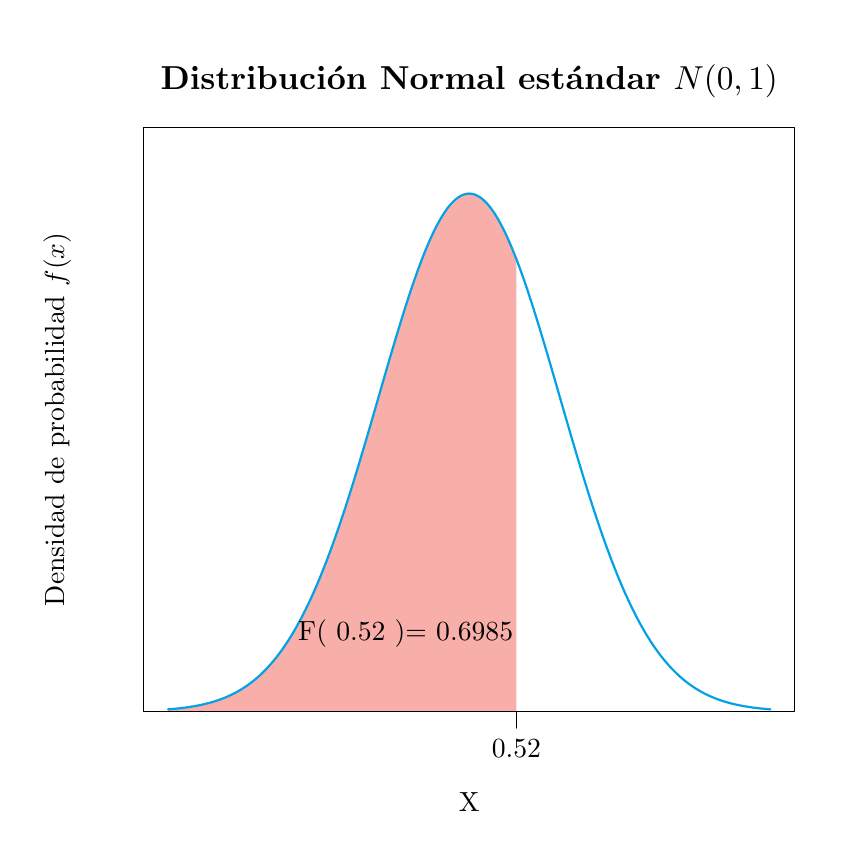
\begin{tikzpicture}[x=1pt,y=1pt]
\definecolor{fillColor}{RGB}{255,255,255}
\path[use as bounding box,fill=fillColor,fill opacity=0.00] (0,0) rectangle (289.08,289.08);
\begin{scope}
\path[clip] (  0.00,  0.00) rectangle (289.08,289.08);
\definecolor{drawColor}{RGB}{0,0,0}

\node[text=drawColor,anchor=base,inner sep=0pt, outer sep=0pt, scale=  1.20] at (159.54,266.89) {\bfseries Distribución Normal estándar $N(0,1)$};

\node[text=drawColor,anchor=base,inner sep=0pt, outer sep=0pt, scale=  1.00] at (159.54,  6.00) {X};

\node[text=drawColor,rotate= 90.00,anchor=base,inner sep=0pt, outer sep=0pt, scale=  1.00] at ( 13.20,147.54) {Densidad de probabilidad $f(x)$};
\end{scope}
\begin{scope}
\path[clip] (  0.00,  0.00) rectangle (289.08,289.08);
\definecolor{drawColor}{RGB}{0,0,0}

\path[draw=drawColor,line width= 0.4pt,line join=round,line cap=round] (176.59, 42.00) -- (176.59, 42.00);

\path[draw=drawColor,line width= 0.4pt,line join=round,line cap=round] (176.59, 42.00) -- (176.59, 36.00);

\node[text=drawColor,anchor=base,inner sep=0pt, outer sep=0pt, scale=  1.00] at (176.59, 25.20) {0.52};
\end{scope}
\begin{scope}
\path[clip] ( 42.00, 42.00) rectangle (277.08,253.08);
\definecolor{fillColor}{RGB}{238,50,36}

\path[fill=fillColor,fill opacity=0.39] ( 50.71, 42.00) --
	( 50.71, 42.76) --
	( 52.02, 42.86) --
	( 53.33, 42.98) --
	( 54.64, 43.12) --
	( 55.95, 43.27) --
	( 57.26, 43.44) --
	( 58.57, 43.63) --
	( 59.89, 43.84) --
	( 61.20, 44.08) --
	( 62.51, 44.34) --
	( 63.82, 44.63) --
	( 65.13, 44.96) --
	( 66.44, 45.32) --
	( 67.75, 45.71) --
	( 69.06, 46.15) --
	( 70.38, 46.63) --
	( 71.69, 47.16) --
	( 73.00, 47.74) --
	( 74.31, 48.37) --
	( 75.62, 49.06) --
	( 76.93, 49.82) --
	( 78.24, 50.64) --
	( 79.55, 51.54) --
	( 80.87, 52.50) --
	( 82.18, 53.55) --
	( 83.49, 54.69) --
	( 84.80, 55.91) --
	( 86.11, 57.23) --
	( 87.42, 58.64) --
	( 88.73, 60.16) --
	( 90.04, 61.78) --
	( 91.36, 63.51) --
	( 92.67, 65.36) --
	( 93.98, 67.33) --
	( 95.29, 69.41) --
	( 96.60, 71.62) --
	( 97.91, 73.96) --
	( 99.22, 76.43) --
	(100.53, 79.03) --
	(101.85, 81.77) --
	(103.16, 84.63) --
	(104.47, 87.63) --
	(105.78, 90.76) --
	(107.09, 94.03) --
	(108.40, 97.42) --
	(109.71,100.95) --
	(111.02,104.59) --
	(112.34,108.35) --
	(113.65,112.23) --
	(114.96,116.22) --
	(116.27,120.30) --
	(117.58,124.48) --
	(118.89,128.75) --
	(120.20,133.09) --
	(121.51,137.49) --
	(122.83,141.94) --
	(124.14,146.44) --
	(125.45,150.96) --
	(126.76,155.50) --
	(128.07,160.04) --
	(129.38,164.56) --
	(130.69,169.05) --
	(132.00,173.50) --
	(133.32,177.88) --
	(134.63,182.19) --
	(135.94,186.40) --
	(137.25,190.50) --
	(138.56,194.48) --
	(139.87,198.30) --
	(141.18,201.97) --
	(142.49,205.47) --
	(143.81,208.77) --
	(145.12,211.87) --
	(146.43,214.74) --
	(147.74,217.39) --
	(149.05,219.79) --
	(150.36,221.94) --
	(151.67,223.82) --
	(152.98,225.43) --
	(154.30,226.75) --
	(155.61,227.79) --
	(156.92,228.53) --
	(158.23,228.98) --
	(159.54,229.13) --
	(160.85,228.98) --
	(162.16,228.53) --
	(163.47,227.79) --
	(164.78,226.75) --
	(166.10,225.43) --
	(167.41,223.82) --
	(168.72,221.94) --
	(170.03,219.79) --
	(171.34,217.39) --
	(172.65,214.74) --
	(173.96,211.87) --
	(175.27,208.77) --
	(176.59,205.47) --
	(176.59, 42.00) --
	cycle;
\definecolor{drawColor}{RGB}{5,161,230}

\path[draw=drawColor,line width= 0.8pt,line join=round,line cap=round] ( 50.71, 42.76) --
	( 52.02, 42.86) --
	( 53.33, 42.98) --
	( 54.64, 43.12) --
	( 55.95, 43.27) --
	( 57.26, 43.44) --
	( 58.57, 43.63) --
	( 59.89, 43.84) --
	( 61.20, 44.08) --
	( 62.51, 44.34) --
	( 63.82, 44.63) --
	( 65.13, 44.96) --
	( 66.44, 45.32) --
	( 67.75, 45.71) --
	( 69.06, 46.15) --
	( 70.38, 46.63) --
	( 71.69, 47.16) --
	( 73.00, 47.74) --
	( 74.31, 48.37) --
	( 75.62, 49.06) --
	( 76.93, 49.82) --
	( 78.24, 50.64) --
	( 79.55, 51.54) --
	( 80.87, 52.50) --
	( 82.18, 53.55) --
	( 83.49, 54.69) --
	( 84.80, 55.91) --
	( 86.11, 57.23) --
	( 87.42, 58.64) --
	( 88.73, 60.16) --
	( 90.04, 61.78) --
	( 91.36, 63.51) --
	( 92.67, 65.36) --
	( 93.98, 67.33) --
	( 95.29, 69.41) --
	( 96.60, 71.62) --
	( 97.91, 73.96) --
	( 99.22, 76.43) --
	(100.53, 79.03) --
	(101.85, 81.77) --
	(103.16, 84.63) --
	(104.47, 87.63) --
	(105.78, 90.76) --
	(107.09, 94.03) --
	(108.40, 97.42) --
	(109.71,100.95) --
	(111.02,104.59) --
	(112.34,108.35) --
	(113.65,112.23) --
	(114.96,116.22) --
	(116.27,120.30) --
	(117.58,124.48) --
	(118.89,128.75) --
	(120.20,133.09) --
	(121.51,137.49) --
	(122.83,141.94) --
	(124.14,146.44) --
	(125.45,150.96) --
	(126.76,155.50) --
	(128.07,160.04) --
	(129.38,164.56) --
	(130.69,169.05) --
	(132.00,173.50) --
	(133.32,177.88) --
	(134.63,182.19) --
	(135.94,186.40) --
	(137.25,190.50) --
	(138.56,194.48) --
	(139.87,198.30) --
	(141.18,201.97) --
	(142.49,205.47) --
	(143.81,208.77) --
	(145.12,211.87) --
	(146.43,214.74) --
	(147.74,217.39) --
	(149.05,219.79) --
	(150.36,221.94) --
	(151.67,223.82) --
	(152.98,225.43) --
	(154.30,226.75) --
	(155.61,227.79) --
	(156.92,228.53) --
	(158.23,228.98) --
	(159.54,229.13) --
	(160.85,228.98) --
	(162.16,228.53) --
	(163.47,227.79) --
	(164.78,226.75) --
	(166.10,225.43) --
	(167.41,223.82) --
	(168.72,221.94) --
	(170.03,219.79) --
	(171.34,217.39) --
	(172.65,214.74) --
	(173.96,211.87) --
	(175.27,208.77) --
	(176.59,205.47) --
	(177.90,201.97) --
	(179.21,198.30) --
	(180.52,194.48) --
	(181.83,190.50) --
	(183.14,186.40) --
	(184.45,182.19) --
	(185.76,177.88) --
	(187.08,173.50) --
	(188.39,169.05) --
	(189.70,164.56) --
	(191.01,160.04) --
	(192.32,155.50) --
	(193.63,150.96) --
	(194.94,146.44) --
	(196.25,141.94) --
	(197.57,137.49) --
	(198.88,133.09) --
	(200.19,128.75) --
	(201.50,124.48) --
	(202.81,120.30) --
	(204.12,116.22) --
	(205.43,112.23) --
	(206.74,108.35) --
	(208.06,104.59) --
	(209.37,100.95) --
	(210.68, 97.42) --
	(211.99, 94.03) --
	(213.30, 90.76) --
	(214.61, 87.63) --
	(215.92, 84.63) --
	(217.23, 81.77) --
	(218.55, 79.03) --
	(219.86, 76.43) --
	(221.17, 73.96) --
	(222.48, 71.62) --
	(223.79, 69.41) --
	(225.10, 67.33) --
	(226.41, 65.36) --
	(227.72, 63.51) --
	(229.04, 61.78) --
	(230.35, 60.16) --
	(231.66, 58.64) --
	(232.97, 57.23) --
	(234.28, 55.91) --
	(235.59, 54.69) --
	(236.90, 53.55) --
	(238.21, 52.50) --
	(239.53, 51.54) --
	(240.84, 50.64) --
	(242.15, 49.82) --
	(243.46, 49.06) --
	(244.77, 48.37) --
	(246.08, 47.74) --
	(247.39, 47.16) --
	(248.70, 46.63) --
	(250.02, 46.15) --
	(251.33, 45.71) --
	(252.64, 45.32) --
	(253.95, 44.96) --
	(255.26, 44.63) --
	(256.57, 44.34) --
	(257.88, 44.08) --
	(259.19, 43.84) --
	(260.51, 43.63) --
	(261.82, 43.44) --
	(263.13, 43.27) --
	(264.44, 43.12) --
	(265.75, 42.98) --
	(267.06, 42.86) --
	(268.37, 42.76);
\definecolor{drawColor}{RGB}{0,0,0}

\node[text=drawColor,anchor=base,inner sep=0pt, outer sep=0pt, scale=  1.00] at (136.59, 67.64) {F( 0.52 )= 0.6985};
\end{scope}
\begin{scope}
\path[clip] (  0.00,  0.00) rectangle (289.08,289.08);
\definecolor{drawColor}{RGB}{0,0,0}

\path[draw=drawColor,line width= 0.4pt,line join=round,line cap=round] ( 42.00, 42.00) --
	(277.08, 42.00) --
	(277.08,253.08) --
	( 42.00,253.08) --
	( 42.00, 42.00);
\end{scope}
\end{tikzpicture}
}}
\end{center}
\end{column}
\end{columns}

\note{
Para evitar tener que calcular probabilidades integrando la función de densidad de la normal estándar se suele utilizar su función de
distribución.

Habitualmente se suele manejar una tabla con los valores de la función de distribución tabulados cada centésima. En esta tabla, la primera
columna contiene las décimas y la primera fila las centésimas, de forma que si por ejemplo queremos medir la probabilidad acumulada hasta el
$0.52$, tenemos que ir hasta la casilla correspondiente a la fila $0.5$  (5 décimas) y hasta la columna $0.02$ (2 centésimas), donde aparece
la probabilidad acumulada $0.6985$ y esta sería el área que queda por debajo de la campana de Gauss de la normal estándar entre $-\infty$ y
$0.52$.
}
\end{frame}


%---------------------------------------------------------------------slide----
\begin{frame}
\frametitle{Cálculo de probabilidades con la Normal estándar}
\framesubtitle{Probabilidades acumuladas por encima de un valor}
Cuando tengamos que calcular probabilidades acumuladas por encima de un determinado valor (cola de acumulación a la derecha), podemos hacerlo por medio de la probabilidad del suceso contrario.
Por ejemplo, 
\[
P(Z>0.52) =1-P(Z\leq 0.52) = 1-F(0.52) = 1 - 0.6985 = 0.3015.
\]
\begin{center}
	\tikzsetnextfilename{variables_aleatorias_continuas/calculo_probabilidades_normal_cola_derecha}
	\mode<article>{\resizebox{0.6\textwidth}{!}{% Created by tikzDevice version 0.10.1 on 2016-05-16 22:15:26
% !TEX encoding = UTF-8 Unicode
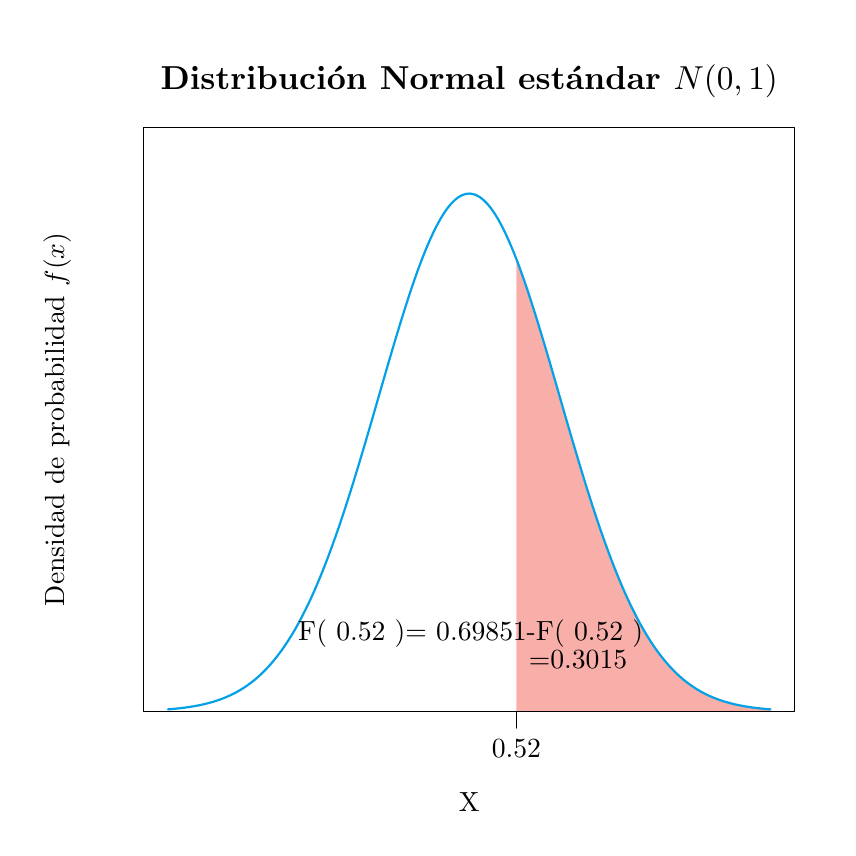
\begin{tikzpicture}[x=1pt,y=1pt]
\definecolor{fillColor}{RGB}{255,255,255}
\path[use as bounding box,fill=fillColor,fill opacity=0.00] (0,0) rectangle (289.08,289.08);
\begin{scope}
\path[clip] (  0.00,  0.00) rectangle (289.08,289.08);
\definecolor{drawColor}{RGB}{0,0,0}

\node[text=drawColor,anchor=base,inner sep=0pt, outer sep=0pt, scale=  1.20] at (159.54,266.89) {\bfseries Distribución Normal estándar $N(0,1)$};

\node[text=drawColor,anchor=base,inner sep=0pt, outer sep=0pt, scale=  1.00] at (159.54,  6.00) {X};

\node[text=drawColor,rotate= 90.00,anchor=base,inner sep=0pt, outer sep=0pt, scale=  1.00] at ( 13.20,147.54) {Densidad de probabilidad $f(x)$};
\end{scope}
\begin{scope}
\path[clip] (  0.00,  0.00) rectangle (289.08,289.08);
\definecolor{drawColor}{RGB}{0,0,0}

\path[draw=drawColor,line width= 0.4pt,line join=round,line cap=round] (176.59, 42.00) -- (176.59, 42.00);

\path[draw=drawColor,line width= 0.4pt,line join=round,line cap=round] (176.59, 42.00) -- (176.59, 36.00);

\node[text=drawColor,anchor=base,inner sep=0pt, outer sep=0pt, scale=  1.00] at (176.59, 25.20) {0.52};
\end{scope}
\begin{scope}
\path[clip] ( 42.00, 42.00) rectangle (277.08,253.08);
\definecolor{fillColor}{RGB}{238,50,36}

\path[fill=fillColor,fill opacity=0.39] (176.59, 42.00) --
	(176.59,205.47) --
	(177.90,201.97) --
	(179.21,198.30) --
	(180.52,194.48) --
	(181.83,190.50) --
	(183.14,186.40) --
	(184.45,182.19) --
	(185.76,177.88) --
	(187.08,173.50) --
	(188.39,169.05) --
	(189.70,164.56) --
	(191.01,160.04) --
	(192.32,155.50) --
	(193.63,150.96) --
	(194.94,146.44) --
	(196.25,141.94) --
	(197.57,137.49) --
	(198.88,133.09) --
	(200.19,128.75) --
	(201.50,124.48) --
	(202.81,120.30) --
	(204.12,116.22) --
	(205.43,112.23) --
	(206.74,108.35) --
	(208.06,104.59) --
	(209.37,100.95) --
	(210.68, 97.42) --
	(211.99, 94.03) --
	(213.30, 90.76) --
	(214.61, 87.63) --
	(215.92, 84.63) --
	(217.23, 81.77) --
	(218.55, 79.03) --
	(219.86, 76.43) --
	(221.17, 73.96) --
	(222.48, 71.62) --
	(223.79, 69.41) --
	(225.10, 67.33) --
	(226.41, 65.36) --
	(227.72, 63.51) --
	(229.04, 61.78) --
	(230.35, 60.16) --
	(231.66, 58.64) --
	(232.97, 57.23) --
	(234.28, 55.91) --
	(235.59, 54.69) --
	(236.90, 53.55) --
	(238.21, 52.50) --
	(239.53, 51.54) --
	(240.84, 50.64) --
	(242.15, 49.82) --
	(243.46, 49.06) --
	(244.77, 48.37) --
	(246.08, 47.74) --
	(247.39, 47.16) --
	(248.70, 46.63) --
	(250.02, 46.15) --
	(251.33, 45.71) --
	(252.64, 45.32) --
	(253.95, 44.96) --
	(255.26, 44.63) --
	(256.57, 44.34) --
	(257.88, 44.08) --
	(259.19, 43.84) --
	(260.51, 43.63) --
	(261.82, 43.44) --
	(263.13, 43.27) --
	(264.44, 43.12) --
	(265.75, 42.98) --
	(267.06, 42.86) --
	(268.37, 42.76) --
	(268.37, 42.00) --
	cycle;
\definecolor{drawColor}{RGB}{5,161,230}

\path[draw=drawColor,line width= 0.8pt,line join=round,line cap=round] ( 50.71, 42.76) --
	( 52.02, 42.86) --
	( 53.33, 42.98) --
	( 54.64, 43.12) --
	( 55.95, 43.27) --
	( 57.26, 43.44) --
	( 58.57, 43.63) --
	( 59.89, 43.84) --
	( 61.20, 44.08) --
	( 62.51, 44.34) --
	( 63.82, 44.63) --
	( 65.13, 44.96) --
	( 66.44, 45.32) --
	( 67.75, 45.71) --
	( 69.06, 46.15) --
	( 70.38, 46.63) --
	( 71.69, 47.16) --
	( 73.00, 47.74) --
	( 74.31, 48.37) --
	( 75.62, 49.06) --
	( 76.93, 49.82) --
	( 78.24, 50.64) --
	( 79.55, 51.54) --
	( 80.87, 52.50) --
	( 82.18, 53.55) --
	( 83.49, 54.69) --
	( 84.80, 55.91) --
	( 86.11, 57.23) --
	( 87.42, 58.64) --
	( 88.73, 60.16) --
	( 90.04, 61.78) --
	( 91.36, 63.51) --
	( 92.67, 65.36) --
	( 93.98, 67.33) --
	( 95.29, 69.41) --
	( 96.60, 71.62) --
	( 97.91, 73.96) --
	( 99.22, 76.43) --
	(100.53, 79.03) --
	(101.85, 81.77) --
	(103.16, 84.63) --
	(104.47, 87.63) --
	(105.78, 90.76) --
	(107.09, 94.03) --
	(108.40, 97.42) --
	(109.71,100.95) --
	(111.02,104.59) --
	(112.34,108.35) --
	(113.65,112.23) --
	(114.96,116.22) --
	(116.27,120.30) --
	(117.58,124.48) --
	(118.89,128.75) --
	(120.20,133.09) --
	(121.51,137.49) --
	(122.83,141.94) --
	(124.14,146.44) --
	(125.45,150.96) --
	(126.76,155.50) --
	(128.07,160.04) --
	(129.38,164.56) --
	(130.69,169.05) --
	(132.00,173.50) --
	(133.32,177.88) --
	(134.63,182.19) --
	(135.94,186.40) --
	(137.25,190.50) --
	(138.56,194.48) --
	(139.87,198.30) --
	(141.18,201.97) --
	(142.49,205.47) --
	(143.81,208.77) --
	(145.12,211.87) --
	(146.43,214.74) --
	(147.74,217.39) --
	(149.05,219.79) --
	(150.36,221.94) --
	(151.67,223.82) --
	(152.98,225.43) --
	(154.30,226.75) --
	(155.61,227.79) --
	(156.92,228.53) --
	(158.23,228.98) --
	(159.54,229.13) --
	(160.85,228.98) --
	(162.16,228.53) --
	(163.47,227.79) --
	(164.78,226.75) --
	(166.10,225.43) --
	(167.41,223.82) --
	(168.72,221.94) --
	(170.03,219.79) --
	(171.34,217.39) --
	(172.65,214.74) --
	(173.96,211.87) --
	(175.27,208.77) --
	(176.59,205.47) --
	(177.90,201.97) --
	(179.21,198.30) --
	(180.52,194.48) --
	(181.83,190.50) --
	(183.14,186.40) --
	(184.45,182.19) --
	(185.76,177.88) --
	(187.08,173.50) --
	(188.39,169.05) --
	(189.70,164.56) --
	(191.01,160.04) --
	(192.32,155.50) --
	(193.63,150.96) --
	(194.94,146.44) --
	(196.25,141.94) --
	(197.57,137.49) --
	(198.88,133.09) --
	(200.19,128.75) --
	(201.50,124.48) --
	(202.81,120.30) --
	(204.12,116.22) --
	(205.43,112.23) --
	(206.74,108.35) --
	(208.06,104.59) --
	(209.37,100.95) --
	(210.68, 97.42) --
	(211.99, 94.03) --
	(213.30, 90.76) --
	(214.61, 87.63) --
	(215.92, 84.63) --
	(217.23, 81.77) --
	(218.55, 79.03) --
	(219.86, 76.43) --
	(221.17, 73.96) --
	(222.48, 71.62) --
	(223.79, 69.41) --
	(225.10, 67.33) --
	(226.41, 65.36) --
	(227.72, 63.51) --
	(229.04, 61.78) --
	(230.35, 60.16) --
	(231.66, 58.64) --
	(232.97, 57.23) --
	(234.28, 55.91) --
	(235.59, 54.69) --
	(236.90, 53.55) --
	(238.21, 52.50) --
	(239.53, 51.54) --
	(240.84, 50.64) --
	(242.15, 49.82) --
	(243.46, 49.06) --
	(244.77, 48.37) --
	(246.08, 47.74) --
	(247.39, 47.16) --
	(248.70, 46.63) --
	(250.02, 46.15) --
	(251.33, 45.71) --
	(252.64, 45.32) --
	(253.95, 44.96) --
	(255.26, 44.63) --
	(256.57, 44.34) --
	(257.88, 44.08) --
	(259.19, 43.84) --
	(260.51, 43.63) --
	(261.82, 43.44) --
	(263.13, 43.27) --
	(264.44, 43.12) --
	(265.75, 42.98) --
	(267.06, 42.86) --
	(268.37, 42.76);
\definecolor{drawColor}{RGB}{0,0,0}

\node[text=drawColor,anchor=base,inner sep=0pt, outer sep=0pt, scale=  1.00] at (136.59, 67.64) {F( 0.52 )= 0.6985};

\node[text=drawColor,anchor=base,inner sep=0pt, outer sep=0pt, scale=  1.00] at (198.88, 67.64) {1-F( 0.52 )};

\node[text=drawColor,anchor=base,inner sep=0pt, outer sep=0pt, scale=  1.00] at (198.88, 57.61) {=0.3015};
\end{scope}
\begin{scope}
\path[clip] (  0.00,  0.00) rectangle (289.08,289.08);
\definecolor{drawColor}{RGB}{0,0,0}

\path[draw=drawColor,line width= 0.4pt,line join=round,line cap=round] ( 42.00, 42.00) --
	(277.08, 42.00) --
	(277.08,253.08) --
	( 42.00,253.08) --
	( 42.00, 42.00);
\end{scope}
\end{tikzpicture}
}}
	\mode<presentation>{\resizebox{0.5\textwidth}{!}{% Created by tikzDevice version 0.10.1 on 2016-05-16 22:15:26
% !TEX encoding = UTF-8 Unicode
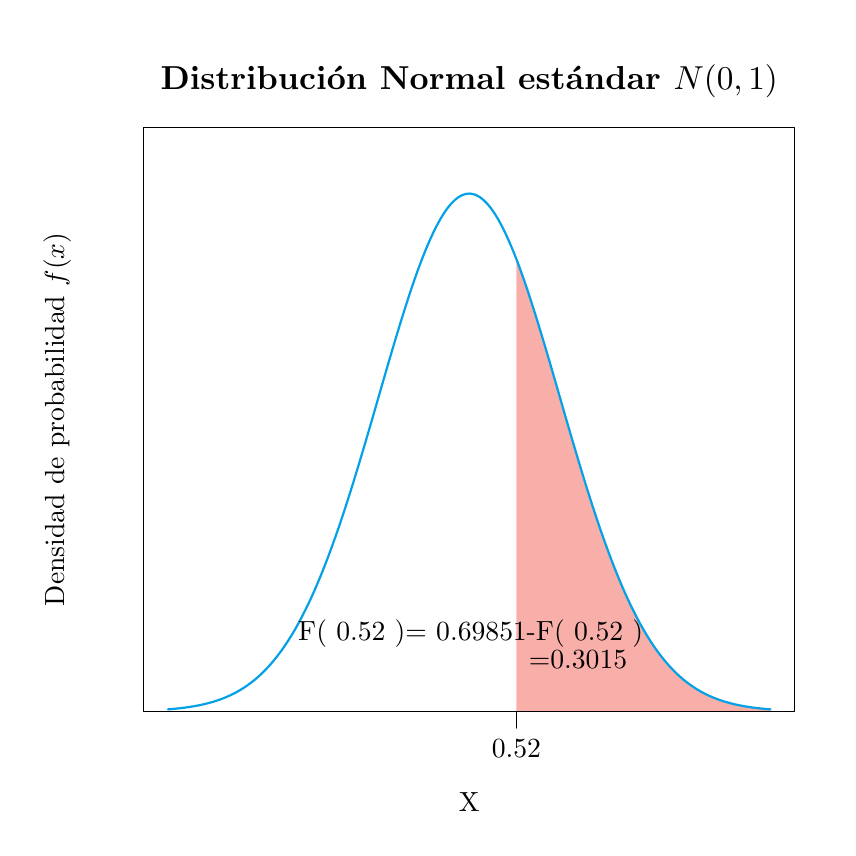
\begin{tikzpicture}[x=1pt,y=1pt]
\definecolor{fillColor}{RGB}{255,255,255}
\path[use as bounding box,fill=fillColor,fill opacity=0.00] (0,0) rectangle (289.08,289.08);
\begin{scope}
\path[clip] (  0.00,  0.00) rectangle (289.08,289.08);
\definecolor{drawColor}{RGB}{0,0,0}

\node[text=drawColor,anchor=base,inner sep=0pt, outer sep=0pt, scale=  1.20] at (159.54,266.89) {\bfseries Distribución Normal estándar $N(0,1)$};

\node[text=drawColor,anchor=base,inner sep=0pt, outer sep=0pt, scale=  1.00] at (159.54,  6.00) {X};

\node[text=drawColor,rotate= 90.00,anchor=base,inner sep=0pt, outer sep=0pt, scale=  1.00] at ( 13.20,147.54) {Densidad de probabilidad $f(x)$};
\end{scope}
\begin{scope}
\path[clip] (  0.00,  0.00) rectangle (289.08,289.08);
\definecolor{drawColor}{RGB}{0,0,0}

\path[draw=drawColor,line width= 0.4pt,line join=round,line cap=round] (176.59, 42.00) -- (176.59, 42.00);

\path[draw=drawColor,line width= 0.4pt,line join=round,line cap=round] (176.59, 42.00) -- (176.59, 36.00);

\node[text=drawColor,anchor=base,inner sep=0pt, outer sep=0pt, scale=  1.00] at (176.59, 25.20) {0.52};
\end{scope}
\begin{scope}
\path[clip] ( 42.00, 42.00) rectangle (277.08,253.08);
\definecolor{fillColor}{RGB}{238,50,36}

\path[fill=fillColor,fill opacity=0.39] (176.59, 42.00) --
	(176.59,205.47) --
	(177.90,201.97) --
	(179.21,198.30) --
	(180.52,194.48) --
	(181.83,190.50) --
	(183.14,186.40) --
	(184.45,182.19) --
	(185.76,177.88) --
	(187.08,173.50) --
	(188.39,169.05) --
	(189.70,164.56) --
	(191.01,160.04) --
	(192.32,155.50) --
	(193.63,150.96) --
	(194.94,146.44) --
	(196.25,141.94) --
	(197.57,137.49) --
	(198.88,133.09) --
	(200.19,128.75) --
	(201.50,124.48) --
	(202.81,120.30) --
	(204.12,116.22) --
	(205.43,112.23) --
	(206.74,108.35) --
	(208.06,104.59) --
	(209.37,100.95) --
	(210.68, 97.42) --
	(211.99, 94.03) --
	(213.30, 90.76) --
	(214.61, 87.63) --
	(215.92, 84.63) --
	(217.23, 81.77) --
	(218.55, 79.03) --
	(219.86, 76.43) --
	(221.17, 73.96) --
	(222.48, 71.62) --
	(223.79, 69.41) --
	(225.10, 67.33) --
	(226.41, 65.36) --
	(227.72, 63.51) --
	(229.04, 61.78) --
	(230.35, 60.16) --
	(231.66, 58.64) --
	(232.97, 57.23) --
	(234.28, 55.91) --
	(235.59, 54.69) --
	(236.90, 53.55) --
	(238.21, 52.50) --
	(239.53, 51.54) --
	(240.84, 50.64) --
	(242.15, 49.82) --
	(243.46, 49.06) --
	(244.77, 48.37) --
	(246.08, 47.74) --
	(247.39, 47.16) --
	(248.70, 46.63) --
	(250.02, 46.15) --
	(251.33, 45.71) --
	(252.64, 45.32) --
	(253.95, 44.96) --
	(255.26, 44.63) --
	(256.57, 44.34) --
	(257.88, 44.08) --
	(259.19, 43.84) --
	(260.51, 43.63) --
	(261.82, 43.44) --
	(263.13, 43.27) --
	(264.44, 43.12) --
	(265.75, 42.98) --
	(267.06, 42.86) --
	(268.37, 42.76) --
	(268.37, 42.00) --
	cycle;
\definecolor{drawColor}{RGB}{5,161,230}

\path[draw=drawColor,line width= 0.8pt,line join=round,line cap=round] ( 50.71, 42.76) --
	( 52.02, 42.86) --
	( 53.33, 42.98) --
	( 54.64, 43.12) --
	( 55.95, 43.27) --
	( 57.26, 43.44) --
	( 58.57, 43.63) --
	( 59.89, 43.84) --
	( 61.20, 44.08) --
	( 62.51, 44.34) --
	( 63.82, 44.63) --
	( 65.13, 44.96) --
	( 66.44, 45.32) --
	( 67.75, 45.71) --
	( 69.06, 46.15) --
	( 70.38, 46.63) --
	( 71.69, 47.16) --
	( 73.00, 47.74) --
	( 74.31, 48.37) --
	( 75.62, 49.06) --
	( 76.93, 49.82) --
	( 78.24, 50.64) --
	( 79.55, 51.54) --
	( 80.87, 52.50) --
	( 82.18, 53.55) --
	( 83.49, 54.69) --
	( 84.80, 55.91) --
	( 86.11, 57.23) --
	( 87.42, 58.64) --
	( 88.73, 60.16) --
	( 90.04, 61.78) --
	( 91.36, 63.51) --
	( 92.67, 65.36) --
	( 93.98, 67.33) --
	( 95.29, 69.41) --
	( 96.60, 71.62) --
	( 97.91, 73.96) --
	( 99.22, 76.43) --
	(100.53, 79.03) --
	(101.85, 81.77) --
	(103.16, 84.63) --
	(104.47, 87.63) --
	(105.78, 90.76) --
	(107.09, 94.03) --
	(108.40, 97.42) --
	(109.71,100.95) --
	(111.02,104.59) --
	(112.34,108.35) --
	(113.65,112.23) --
	(114.96,116.22) --
	(116.27,120.30) --
	(117.58,124.48) --
	(118.89,128.75) --
	(120.20,133.09) --
	(121.51,137.49) --
	(122.83,141.94) --
	(124.14,146.44) --
	(125.45,150.96) --
	(126.76,155.50) --
	(128.07,160.04) --
	(129.38,164.56) --
	(130.69,169.05) --
	(132.00,173.50) --
	(133.32,177.88) --
	(134.63,182.19) --
	(135.94,186.40) --
	(137.25,190.50) --
	(138.56,194.48) --
	(139.87,198.30) --
	(141.18,201.97) --
	(142.49,205.47) --
	(143.81,208.77) --
	(145.12,211.87) --
	(146.43,214.74) --
	(147.74,217.39) --
	(149.05,219.79) --
	(150.36,221.94) --
	(151.67,223.82) --
	(152.98,225.43) --
	(154.30,226.75) --
	(155.61,227.79) --
	(156.92,228.53) --
	(158.23,228.98) --
	(159.54,229.13) --
	(160.85,228.98) --
	(162.16,228.53) --
	(163.47,227.79) --
	(164.78,226.75) --
	(166.10,225.43) --
	(167.41,223.82) --
	(168.72,221.94) --
	(170.03,219.79) --
	(171.34,217.39) --
	(172.65,214.74) --
	(173.96,211.87) --
	(175.27,208.77) --
	(176.59,205.47) --
	(177.90,201.97) --
	(179.21,198.30) --
	(180.52,194.48) --
	(181.83,190.50) --
	(183.14,186.40) --
	(184.45,182.19) --
	(185.76,177.88) --
	(187.08,173.50) --
	(188.39,169.05) --
	(189.70,164.56) --
	(191.01,160.04) --
	(192.32,155.50) --
	(193.63,150.96) --
	(194.94,146.44) --
	(196.25,141.94) --
	(197.57,137.49) --
	(198.88,133.09) --
	(200.19,128.75) --
	(201.50,124.48) --
	(202.81,120.30) --
	(204.12,116.22) --
	(205.43,112.23) --
	(206.74,108.35) --
	(208.06,104.59) --
	(209.37,100.95) --
	(210.68, 97.42) --
	(211.99, 94.03) --
	(213.30, 90.76) --
	(214.61, 87.63) --
	(215.92, 84.63) --
	(217.23, 81.77) --
	(218.55, 79.03) --
	(219.86, 76.43) --
	(221.17, 73.96) --
	(222.48, 71.62) --
	(223.79, 69.41) --
	(225.10, 67.33) --
	(226.41, 65.36) --
	(227.72, 63.51) --
	(229.04, 61.78) --
	(230.35, 60.16) --
	(231.66, 58.64) --
	(232.97, 57.23) --
	(234.28, 55.91) --
	(235.59, 54.69) --
	(236.90, 53.55) --
	(238.21, 52.50) --
	(239.53, 51.54) --
	(240.84, 50.64) --
	(242.15, 49.82) --
	(243.46, 49.06) --
	(244.77, 48.37) --
	(246.08, 47.74) --
	(247.39, 47.16) --
	(248.70, 46.63) --
	(250.02, 46.15) --
	(251.33, 45.71) --
	(252.64, 45.32) --
	(253.95, 44.96) --
	(255.26, 44.63) --
	(256.57, 44.34) --
	(257.88, 44.08) --
	(259.19, 43.84) --
	(260.51, 43.63) --
	(261.82, 43.44) --
	(263.13, 43.27) --
	(264.44, 43.12) --
	(265.75, 42.98) --
	(267.06, 42.86) --
	(268.37, 42.76);
\definecolor{drawColor}{RGB}{0,0,0}

\node[text=drawColor,anchor=base,inner sep=0pt, outer sep=0pt, scale=  1.00] at (136.59, 67.64) {F( 0.52 )= 0.6985};

\node[text=drawColor,anchor=base,inner sep=0pt, outer sep=0pt, scale=  1.00] at (198.88, 67.64) {1-F( 0.52 )};

\node[text=drawColor,anchor=base,inner sep=0pt, outer sep=0pt, scale=  1.00] at (198.88, 57.61) {=0.3015};
\end{scope}
\begin{scope}
\path[clip] (  0.00,  0.00) rectangle (289.08,289.08);
\definecolor{drawColor}{RGB}{0,0,0}

\path[draw=drawColor,line width= 0.4pt,line join=round,line cap=round] ( 42.00, 42.00) --
	(277.08, 42.00) --
	(277.08,253.08) --
	( 42.00,253.08) --
	( 42.00, 42.00);
\end{scope}
\end{tikzpicture}
}}
\end{center}

\note{
Cuando tengamos que calcular probabilidades acumuladas por encima de un determinado valor, podemos hacerlo por medio de la probabilidad del
suceso contrario, ya que la función de distribución siempre mide probabilidades acumuladas por debajo de cada valor. 

Así, la probabilidad acumulada por encima de $0.52$, será 1 menos la probabilidad acumulada por debajo de dicho valor, que como hemos visto
en la tabla, valía $0.6985$, lo que nos da $0.3015$. Esto es lógico, ya que si el área total por debajo de la campana de Gauss es 1, el área
acumulada por encima de $0.52$ será 1 menos el área que quede por debajo de este valor. 
}
\end{frame}


%---------------------------------------------------------------------slide----
\begin{frame}
\frametitle{Tipificación}
Ya se ha visto cómo calcular probabilidades con una distribución normal estándar, pero \emph{¿qué hacer cuando la distribución normal no es la estándar?}
En tal caso hay que transformar la variable normal en una normal estándar.

\begin{teorema}[Tipificación]
Si $X$ es una variable que sigue una distribución de probabilidad Normal de media $\mu$ y desviación típica $\sigma$, $X\sim N(\mu,\sigma)$, entonces la variable resultante de restarle a $X$ su media $\mu$ y dividir por su desviación típica $\sigma$, sigue un modelo de distribución de probabilidad Normal estándar,
\[
X\sim N(\mu,\sigma) \Rightarrow Z=\frac{X-\mu}{\sigma}\sim N(0,1).
\]
Esta transformación lineal se conoce como \emph{transformación de tipificación} y la variable resultante $Z$ se conoce como \emph{normal
tipificada}.
\end{teorema} 

Así pues, para calcular probabilidades de una variable Normal que no sea la Normal estándar, se aplica primero la transformación de tipificación y después se puede utilizar la función de distribución de la Normal estándar.

\note{
Ya se ha visto cómo calcular probabilidades con una distribución normal estándar, pero \emph{¿qué hacer cuando la
distribución normal no es la estándar?}
En tal caso hay que transformar la variable normal en una normal estándar.
\begin{teorema}[Tipificación]
Si $X$ es una variable normal de media $\mu$ y desviación típica $\sigma$, entonces la variable resultante de restarle a $X$ su media y
dividir por su desviación típica, sigue un modelo de distribución normal estándar:
\[
X\sim N(\mu,\sigma) \Rightarrow Z=\frac{X-\mu}{\sigma}\sim N(0,1).
\]
Esta transformación lineal se conoce como \emph{transformación de tipificación} y la variable resultante $Z$ se conoce como \emph{normal
tipificada}.
\end{teorema} 

Así pues, para calcular probabilidades de una variable normal que no sea la normal estándar, tendremos que aplicar la transformación de
tipificación primero y después se puede utilizar la tabla de la función de distribución de la normal estándar.
}
\end{frame}


%---------------------------------------------------------------------slide----
\begin{frame}
\frametitle{Cálculo de probabilidades tipificando}
\framesubtitle{Ejemplo}
Supóngase que la nota de un examen sigue un modelo de distribución de probabilidad normal $N(\mu=6,\sigma=1.5)$. 
¿Qué porcentaje de suspensos habrá en la población?

Como $X$ no es la normal estándar, primero se le aplica la
transformación de tipificación $Z=\displaystyle \frac{X-\mu}{\sigma} = \frac{X-6}{1.5}$,
\[
P(X<5) = P\left(\frac{X-6}{1.5}<\frac{5-6}{1.5}\right) = P(Z<-0.67).
\]
Después se puede usar la tabla de la función de distribución de la Normal estándar:
\[
P(Z<-0.67) = F(-0.67) = 0.2514.
\]

Así pues, habrán suspendido el $25.14\%$ de los alumnos. 

\note{
Veamos un ejemplo. 

Supóngase que la nota de un examen sigue un modelo de distribución de probabilidad normal $N(\mu=6,\sigma=1.5)$. \emph{¿Qué porcentaje de
suspensos habrá en la población?}

Para responder a esta pregunta necesitamos calcular la probabilidad de que la nota sea inferior a 5. Como $X$ no es la normal estándar, se
le aplica la transformación de tipificación, que es $Z=\displaystyle \frac{X-\mu}{\sigma} = \frac{X-6}{1.5}$. Por tanto, 
\[
P(X<5) = P\left(\frac{X-6}{1.5}<\frac{5-6}{1.5}\right) = P(Z<-0.67).
\]
Después sólo queda mirar en tabla de la función de distribución de la normal estándar y observar que la probabilidad acumulada hasta el
$-0.67$ es $0.2514$.

Así pues, habrán suspendido el $25.14\%$ de los alumnos. 
}
\end{frame}


\subsection{Distribución Chi-cuadrado}

%---------------------------------------------------------------------slide----
\begin{frame}
\frametitle{Distribución de probabilidad chi-cuadrado $\chi^2(n)$}
\begin{definicion}[Distribución de probabilidad Chi-cuadrado $\chi^2(n)$]
Dadas $n$ variables aleatorias independientes $Z_1,\ldots,Z_n$, todas ellas siguiendo un modelo de distribución Normal estándar, entonces la variable
\[
\chi^2(n) = Z_1^2+\cdots +Z_n^2.
\]
sigue un modelo de distribución de probabilidad \emph{chi-cuadrado de $n$ grados de libertad}.
\end{definicion}

Su rango es $\mathbb{R}^+$ y su media y varianza valen
\[
\mu = n, \qquad \sigma^2 = 2n.
\]

Como se verá más adelante, la distribución chi-cuadrado juega un papel importante en la estimación de la varianza poblacional y en el
estudio de la relación entre variables cualitativas.

\note{
Las distribuciones que veremos a continuación son distribuciones que siguen algunos de los estadísticos observados en las muestras
aleatorias. Su principal utilidad se verá en el siguiente tema.

El primer modelo de distribución es el modelo chi-cuadrado.

Si  $Z_1,\ldots,Z_n$ son $n$ variables aleatorias normales estándar independientes, entonces
la suma de sus cuadrados sigue un modelo de distribución \emph{chi-cuadrado de $n$ grados de libertad}:
\[
\chi^2(n) = Z_1^2+\cdots +Z_n^2.
\]

Se cumple que su recorrido es  $\mathbb{R}^+$, su media vale $\mu=n$ y su varianza vale $\sigma^2 = 2n$.

Como se verá más adelante, la distribución chi-cuadrado juega un papel importante en la estimación de la varianza poblacional y en el
estudio de la relación entre variables cualitativas.
}
\end{frame}


%---------------------------------------------------------------------slide----
\begin{frame}
\frametitle{Función de densidad de la distribución chi-cuadrado}

\begin{center}
	\tikzsetnextfilename{variables_aleatorias_continuas/funcion_densidad_chi_cuadrado}
	\mode<article>{\resizebox{0.6\textwidth}{!}{%% Input file name: funcion_densidad_chi_cuadrado.fig
%% FIG version: 3.2
%% Orientation: Landscape
%% Justification: Flush Left
%% Units: Inches
%% Paper size: A4
%% Magnification: 100.0
%% Resolution: 1200ppi

\begin{pspicture}(6.68cm,3.48cm)(16.80cm,13.45cm)
\psset{unit=0.8cm}
%%
%% Depth: 2147483647
%%
\newrgbcolor{mycolor0}{1.00 0.50 0.31}\definecolor{mycolor0}{rgb}{1.00,0.50,0.31}
\newrgbcolor{mycolor1}{0.28 0.46 1.00}\definecolor{mycolor1}{rgb}{0.28,0.46,1.00}
\newrgbcolor{mycolor2}{0.56 0.93 0.56}\definecolor{mycolor2}{rgb}{0.56,0.93,0.56}
\newgray{mycolor3}{0.74}\definecolor{mycolor3}{gray}{0.74}
%%
%% Depth: 100
%%
\psset{linestyle=solid,linewidth=0.03175,linecolor=mycolor0,fillstyle=none}
\psline(10.91,15.28)(10.99,13.55)(11.08,12.15)(11.17,11.12)(11.27,10.34)(11.36,9.73)(11.46,9.25)(11.55,8.86)(11.64,8.54)(11.74,8.27)(11.83,8.05)(11.93,7.87)(12.02,7.71)(12.12,7.58)(12.21,7.47)(12.30,7.38)(12.40,7.30)(12.49,7.23)(12.59,7.17)(12.68,7.12)(12.78,7.08)(12.87,7.04)(12.96,7.01)(13.06,6.98)(13.15,6.96)(13.25,6.94)(13.34,6.92)(13.43,6.90)(13.53,6.89)(13.62,6.88)(13.72,6.87)(13.81,6.86)(13.91,6.85)(14.00,6.85)(14.09,6.84)(14.19,6.83)(14.28,6.83)(14.38,6.83)(14.47,6.82)(14.56,6.82)(14.66,6.82)(14.76,6.82)(14.85,6.81)(14.94,6.81)(15.04,6.81)(15.13,6.81)(15.23,6.81)(15.32,6.81)(15.41,6.81)(15.51,6.81)(15.60,6.81)(15.70,6.80)(15.79,6.80)(15.89,6.80)(15.98,6.80)(16.07,6.80)(16.17,6.80)(16.26,6.80)(16.36,6.80)(16.45,6.80)(16.54,6.80)(16.64,6.80)(16.73,6.80)(16.83,6.80)(16.92,6.80)(17.02,6.80)(17.11,6.80)(17.20,6.80)(17.30,6.80)(17.39,6.80)(17.49,6.80)(17.58,6.80)(17.68,6.80)(17.77,6.80)(17.86,6.80)(17.96,6.80)(18.05,6.80)(18.15,6.80)(18.24,6.80)(18.33,6.80)(18.43,6.80)(18.52,6.80)(18.62,6.80)(18.71,6.80)(18.81,6.80)(18.90,6.80)(18.99,6.80)(19.09,6.80)(19.18,6.80)(19.28,6.80)(19.37,6.80)(19.47,6.80)(19.56,6.80)(19.66,6.80)(19.75,6.80)(19.84,6.80)(19.94,6.80)
\psset{linecolor=black}
\psline(10.61,6.47)(20.28,6.47)
\psline(10.61,6.47)(10.61,6.26)
\psline(12.54,6.47)(12.54,6.26)
\psline(14.48,6.47)(14.48,6.26)
\psline(16.41,6.47)(16.41,6.26)
\psline(18.35,6.47)(18.35,6.26)
\psline(20.28,6.47)(20.28,6.26)
\rput(10.61,5.71){0}
\rput(12.54,5.71){5}
\rput(14.48,5.71){10}
\rput(16.41,5.71){15}
\rput(18.35,5.71){20}
\rput(20.28,5.71){25}
\psline(10.23,6.80)(10.23,14.95)
\psline(10.23,6.80)(10.02,6.80)
\psline(10.23,8.16)(10.02,8.16)
\psline(10.23,9.52)(10.02,9.52)
\psline(10.23,10.88)(10.02,10.88)
\psline(10.23,12.23)(10.02,12.23)
\psline(10.23,13.59)(10.02,13.59)
\psline(10.23,14.95)(10.02,14.95)
\rput{90}(9.73,6.80){0.00}
\rput{90}(9.73,8.16){0.05}
\rput{90}(9.73,9.52){0.10}
\rput{90}(9.73,10.88){0.15}
\rput{90}(9.73,12.23){0.20}
\rput{90}(9.73,13.59){0.25}
\rput{90}(9.73,14.95){0.30}
\psline(10.23,6.47)(20.31,6.47)(20.31,15.28)(10.23,15.28)(10.23,6.47)
\rput(15.27,15.99){Distintas distribuciones chi-cuadrado}
\rput(15.27,4.86){$X$}
\rput[l]{90}(8.86,9.54){Densidad $f(x)$}
\psset{linecolor=mycolor1}
\psline(10.61,6.80)(10.70,11.54)(10.80,12.73)(10.89,13.23)(10.99,13.38)(11.08,13.31)(11.17,13.11)(11.27,12.84)(11.36,12.51)(11.46,12.16)(11.55,11.81)(11.64,11.45)(11.74,11.10)(11.83,10.76)(11.93,10.44)(12.02,10.14)(12.12,9.85)(12.21,9.58)(12.30,9.34)(12.40,9.11)(12.49,8.90)(12.59,8.70)(12.68,8.52)(12.78,8.36)(12.87,8.21)(12.96,8.08)(13.06,7.95)(13.15,7.84)(13.25,7.74)(13.34,7.64)(13.43,7.56)(13.53,7.48)(13.62,7.41)(13.72,7.35)(13.81,7.30)(13.91,7.25)(14.00,7.20)(14.09,7.16)(14.19,7.12)(14.28,7.09)(14.38,7.06)(14.47,7.03)(14.56,7.01)(14.66,6.99)(14.76,6.97)(14.85,6.95)(14.94,6.93)(15.04,6.92)(15.13,6.91)(15.23,6.90)(15.32,6.89)(15.41,6.88)(15.51,6.87)(15.60,6.86)(15.70,6.85)(15.79,6.85)(15.89,6.84)(15.98,6.84)(16.07,6.83)(16.17,6.83)(16.26,6.83)(16.36,6.82)(16.45,6.82)(16.54,6.82)(16.64,6.82)(16.73,6.82)(16.83,6.81)(16.92,6.81)(17.02,6.81)(17.11,6.81)(17.20,6.81)(17.30,6.81)(17.39,6.81)(17.49,6.81)(17.58,6.81)(17.68,6.81)(17.77,6.80)(17.86,6.80)(17.96,6.80)(18.05,6.80)(18.15,6.80)(18.24,6.80)(18.33,6.80)(18.43,6.80)(18.52,6.80)(18.62,6.80)(18.71,6.80)(18.81,6.80)(18.90,6.80)(18.99,6.80)(19.09,6.80)(19.18,6.80)(19.28,6.80)(19.37,6.80)(19.47,6.80)(19.56,6.80)(19.66,6.80)(19.75,6.80)(19.84,6.80)(19.94,6.80)
\psset{linecolor=mycolor2}
\psline(10.61,6.80)(10.70,6.80)(10.80,6.80)(10.89,6.81)(10.99,6.82)(11.08,6.84)(11.17,6.88)(11.27,6.93)(11.36,6.99)(11.46,7.07)(11.55,7.17)(11.64,7.28)(11.74,7.40)(11.83,7.53)(11.93,7.67)(12.02,7.81)(12.12,7.96)(12.21,8.11)(12.30,8.26)(12.40,8.40)(12.49,8.54)(12.59,8.68)(12.68,8.80)(12.78,8.92)(12.87,9.02)(12.96,9.11)(13.06,9.20)(13.15,9.27)(13.25,9.33)(13.34,9.37)(13.43,9.41)(13.53,9.44)(13.62,9.45)(13.72,9.45)(13.81,9.45)(13.91,9.43)(14.00,9.41)(14.09,9.38)(14.19,9.34)(14.28,9.29)(14.38,9.24)(14.47,9.19)(14.56,9.13)(14.66,9.07)(14.76,9.00)(14.85,8.93)(14.94,8.86)(15.04,8.79)(15.13,8.71)(15.23,8.64)(15.32,8.57)(15.41,8.49)(15.51,8.42)(15.60,8.35)(15.70,8.28)(15.79,8.21)(15.89,8.14)(15.98,8.07)(16.07,8.01)(16.17,7.94)(16.26,7.88)(16.36,7.83)(16.45,7.77)(16.54,7.71)(16.64,7.66)(16.73,7.61)(16.83,7.56)(16.92,7.52)(17.02,7.47)(17.11,7.43)(17.20,7.39)(17.30,7.36)(17.39,7.32)(17.49,7.29)(17.58,7.26)(17.68,7.23)(17.77,7.20)(17.86,7.17)(17.96,7.15)(18.05,7.12)(18.15,7.10)(18.24,7.08)(18.33,7.06)(18.43,7.04)(18.52,7.02)(18.62,7.01)(18.71,6.99)(18.81,6.98)(18.90,6.97)(18.99,6.95)(19.09,6.94)(19.18,6.93)(19.28,6.92)(19.37,6.91)(19.47,6.90)(19.56,6.90)(19.66,6.89)(19.75,6.88)(19.84,6.87)(19.94,6.87)
\psset{linecolor=mycolor3}
\psline(10.23,6.80)(20.31,6.80)
\psset{linecolor=mycolor0}
\psline(18.17,14.53)(18.80,14.53)
\psset{linecolor=mycolor1}
\psline(18.17,14.11)(18.80,14.11)
\psset{linecolor=mycolor2}
\psline(18.17,13.68)(18.80,13.68)
\rput[lb](19,14.33){$\chi^2(1)$}
\rput[lb](19,13.91){$\chi^2(3)$}
\rput[lb](19,13.49){$\chi^2(10)$}
\end{pspicture}
%% End
}}
	\mode<presentation>{\resizebox{0.6\textwidth}{!}{%% Input file name: funcion_densidad_chi_cuadrado.fig
%% FIG version: 3.2
%% Orientation: Landscape
%% Justification: Flush Left
%% Units: Inches
%% Paper size: A4
%% Magnification: 100.0
%% Resolution: 1200ppi

\begin{pspicture}(6.68cm,3.48cm)(16.80cm,13.45cm)
\psset{unit=0.8cm}
%%
%% Depth: 2147483647
%%
\newrgbcolor{mycolor0}{1.00 0.50 0.31}\definecolor{mycolor0}{rgb}{1.00,0.50,0.31}
\newrgbcolor{mycolor1}{0.28 0.46 1.00}\definecolor{mycolor1}{rgb}{0.28,0.46,1.00}
\newrgbcolor{mycolor2}{0.56 0.93 0.56}\definecolor{mycolor2}{rgb}{0.56,0.93,0.56}
\newgray{mycolor3}{0.74}\definecolor{mycolor3}{gray}{0.74}
%%
%% Depth: 100
%%
\psset{linestyle=solid,linewidth=0.03175,linecolor=mycolor0,fillstyle=none}
\psline(10.91,15.28)(10.99,13.55)(11.08,12.15)(11.17,11.12)(11.27,10.34)(11.36,9.73)(11.46,9.25)(11.55,8.86)(11.64,8.54)(11.74,8.27)(11.83,8.05)(11.93,7.87)(12.02,7.71)(12.12,7.58)(12.21,7.47)(12.30,7.38)(12.40,7.30)(12.49,7.23)(12.59,7.17)(12.68,7.12)(12.78,7.08)(12.87,7.04)(12.96,7.01)(13.06,6.98)(13.15,6.96)(13.25,6.94)(13.34,6.92)(13.43,6.90)(13.53,6.89)(13.62,6.88)(13.72,6.87)(13.81,6.86)(13.91,6.85)(14.00,6.85)(14.09,6.84)(14.19,6.83)(14.28,6.83)(14.38,6.83)(14.47,6.82)(14.56,6.82)(14.66,6.82)(14.76,6.82)(14.85,6.81)(14.94,6.81)(15.04,6.81)(15.13,6.81)(15.23,6.81)(15.32,6.81)(15.41,6.81)(15.51,6.81)(15.60,6.81)(15.70,6.80)(15.79,6.80)(15.89,6.80)(15.98,6.80)(16.07,6.80)(16.17,6.80)(16.26,6.80)(16.36,6.80)(16.45,6.80)(16.54,6.80)(16.64,6.80)(16.73,6.80)(16.83,6.80)(16.92,6.80)(17.02,6.80)(17.11,6.80)(17.20,6.80)(17.30,6.80)(17.39,6.80)(17.49,6.80)(17.58,6.80)(17.68,6.80)(17.77,6.80)(17.86,6.80)(17.96,6.80)(18.05,6.80)(18.15,6.80)(18.24,6.80)(18.33,6.80)(18.43,6.80)(18.52,6.80)(18.62,6.80)(18.71,6.80)(18.81,6.80)(18.90,6.80)(18.99,6.80)(19.09,6.80)(19.18,6.80)(19.28,6.80)(19.37,6.80)(19.47,6.80)(19.56,6.80)(19.66,6.80)(19.75,6.80)(19.84,6.80)(19.94,6.80)
\psset{linecolor=black}
\psline(10.61,6.47)(20.28,6.47)
\psline(10.61,6.47)(10.61,6.26)
\psline(12.54,6.47)(12.54,6.26)
\psline(14.48,6.47)(14.48,6.26)
\psline(16.41,6.47)(16.41,6.26)
\psline(18.35,6.47)(18.35,6.26)
\psline(20.28,6.47)(20.28,6.26)
\rput(10.61,5.71){0}
\rput(12.54,5.71){5}
\rput(14.48,5.71){10}
\rput(16.41,5.71){15}
\rput(18.35,5.71){20}
\rput(20.28,5.71){25}
\psline(10.23,6.80)(10.23,14.95)
\psline(10.23,6.80)(10.02,6.80)
\psline(10.23,8.16)(10.02,8.16)
\psline(10.23,9.52)(10.02,9.52)
\psline(10.23,10.88)(10.02,10.88)
\psline(10.23,12.23)(10.02,12.23)
\psline(10.23,13.59)(10.02,13.59)
\psline(10.23,14.95)(10.02,14.95)
\rput{90}(9.73,6.80){0.00}
\rput{90}(9.73,8.16){0.05}
\rput{90}(9.73,9.52){0.10}
\rput{90}(9.73,10.88){0.15}
\rput{90}(9.73,12.23){0.20}
\rput{90}(9.73,13.59){0.25}
\rput{90}(9.73,14.95){0.30}
\psline(10.23,6.47)(20.31,6.47)(20.31,15.28)(10.23,15.28)(10.23,6.47)
\rput(15.27,15.99){Distintas distribuciones chi-cuadrado}
\rput(15.27,4.86){$X$}
\rput[l]{90}(8.86,9.54){Densidad $f(x)$}
\psset{linecolor=mycolor1}
\psline(10.61,6.80)(10.70,11.54)(10.80,12.73)(10.89,13.23)(10.99,13.38)(11.08,13.31)(11.17,13.11)(11.27,12.84)(11.36,12.51)(11.46,12.16)(11.55,11.81)(11.64,11.45)(11.74,11.10)(11.83,10.76)(11.93,10.44)(12.02,10.14)(12.12,9.85)(12.21,9.58)(12.30,9.34)(12.40,9.11)(12.49,8.90)(12.59,8.70)(12.68,8.52)(12.78,8.36)(12.87,8.21)(12.96,8.08)(13.06,7.95)(13.15,7.84)(13.25,7.74)(13.34,7.64)(13.43,7.56)(13.53,7.48)(13.62,7.41)(13.72,7.35)(13.81,7.30)(13.91,7.25)(14.00,7.20)(14.09,7.16)(14.19,7.12)(14.28,7.09)(14.38,7.06)(14.47,7.03)(14.56,7.01)(14.66,6.99)(14.76,6.97)(14.85,6.95)(14.94,6.93)(15.04,6.92)(15.13,6.91)(15.23,6.90)(15.32,6.89)(15.41,6.88)(15.51,6.87)(15.60,6.86)(15.70,6.85)(15.79,6.85)(15.89,6.84)(15.98,6.84)(16.07,6.83)(16.17,6.83)(16.26,6.83)(16.36,6.82)(16.45,6.82)(16.54,6.82)(16.64,6.82)(16.73,6.82)(16.83,6.81)(16.92,6.81)(17.02,6.81)(17.11,6.81)(17.20,6.81)(17.30,6.81)(17.39,6.81)(17.49,6.81)(17.58,6.81)(17.68,6.81)(17.77,6.80)(17.86,6.80)(17.96,6.80)(18.05,6.80)(18.15,6.80)(18.24,6.80)(18.33,6.80)(18.43,6.80)(18.52,6.80)(18.62,6.80)(18.71,6.80)(18.81,6.80)(18.90,6.80)(18.99,6.80)(19.09,6.80)(19.18,6.80)(19.28,6.80)(19.37,6.80)(19.47,6.80)(19.56,6.80)(19.66,6.80)(19.75,6.80)(19.84,6.80)(19.94,6.80)
\psset{linecolor=mycolor2}
\psline(10.61,6.80)(10.70,6.80)(10.80,6.80)(10.89,6.81)(10.99,6.82)(11.08,6.84)(11.17,6.88)(11.27,6.93)(11.36,6.99)(11.46,7.07)(11.55,7.17)(11.64,7.28)(11.74,7.40)(11.83,7.53)(11.93,7.67)(12.02,7.81)(12.12,7.96)(12.21,8.11)(12.30,8.26)(12.40,8.40)(12.49,8.54)(12.59,8.68)(12.68,8.80)(12.78,8.92)(12.87,9.02)(12.96,9.11)(13.06,9.20)(13.15,9.27)(13.25,9.33)(13.34,9.37)(13.43,9.41)(13.53,9.44)(13.62,9.45)(13.72,9.45)(13.81,9.45)(13.91,9.43)(14.00,9.41)(14.09,9.38)(14.19,9.34)(14.28,9.29)(14.38,9.24)(14.47,9.19)(14.56,9.13)(14.66,9.07)(14.76,9.00)(14.85,8.93)(14.94,8.86)(15.04,8.79)(15.13,8.71)(15.23,8.64)(15.32,8.57)(15.41,8.49)(15.51,8.42)(15.60,8.35)(15.70,8.28)(15.79,8.21)(15.89,8.14)(15.98,8.07)(16.07,8.01)(16.17,7.94)(16.26,7.88)(16.36,7.83)(16.45,7.77)(16.54,7.71)(16.64,7.66)(16.73,7.61)(16.83,7.56)(16.92,7.52)(17.02,7.47)(17.11,7.43)(17.20,7.39)(17.30,7.36)(17.39,7.32)(17.49,7.29)(17.58,7.26)(17.68,7.23)(17.77,7.20)(17.86,7.17)(17.96,7.15)(18.05,7.12)(18.15,7.10)(18.24,7.08)(18.33,7.06)(18.43,7.04)(18.52,7.02)(18.62,7.01)(18.71,6.99)(18.81,6.98)(18.90,6.97)(18.99,6.95)(19.09,6.94)(19.18,6.93)(19.28,6.92)(19.37,6.91)(19.47,6.90)(19.56,6.90)(19.66,6.89)(19.75,6.88)(19.84,6.87)(19.94,6.87)
\psset{linecolor=mycolor3}
\psline(10.23,6.80)(20.31,6.80)
\psset{linecolor=mycolor0}
\psline(18.17,14.53)(18.80,14.53)
\psset{linecolor=mycolor1}
\psline(18.17,14.11)(18.80,14.11)
\psset{linecolor=mycolor2}
\psline(18.17,13.68)(18.80,13.68)
\rput[lb](19,14.33){$\chi^2(1)$}
\rput[lb](19,13.91){$\chi^2(3)$}
\rput[lb](19,13.49){$\chi^2(10)$}
\end{pspicture}
%% End
}}
\end{center}

\note{
Aquí tenemos las gráfica de la función de densidad de varias distribuciones chi-cuadrado con distintos grados de libertad. Como se puede
apreciar, esta distribución, por ser la suma de cuadrados, no presenta valores negativos, y a diferencia de la normal, siempre es asimétrica
hacia la izquierda.
}
\end{frame}


%---------------------------------------------------------------------slide----
\begin{frame}
\frametitle{Propiedades de la distribución chi-cuadrado $\chi^2(n)$}
\begin{itemize}
\item No toma valores negativos.
\item Si $X\sim \chi^2(n)$ e $Y\sim \chi^2(m)$, entonces
\[
X+Y \sim \chi^2(n+m).
\]
\item Al aumentar el número de grados de libertad, se aproxima asintóticamente a una normal.
\end{itemize}

\note{
Algunas propiedades que tiene la distribución chi-cuadrado son:
\begin{itemize}
\item No toma valores negativos.
\item Si $X\sim \chi^2(n)$ e $Y\sim \chi^2(m)$, entonces
\[
X+Y \sim \chi^2(n+m).
\]
\item Al aumentar el número de grados de libertad, se aproxima asintóticamente a una normal.
\end{itemize}
}
\end{frame}


\subsection{Distribución T de Student}

%---------------------------------------------------------------------slide----
\begin{frame}
\frametitle{Distribución de probabilidad T de Student $T(n)$}

\begin{definicion}[Distribución de probabilidad T de Student $T(n)$]
Dada una variable $Z$ que sigue un modelo de distribución de probabilidad Normal estándar, $Z\sim N(0,1)$, y una variable $X$ que sigue un modelo de distribución de probabilidad Chi-cuadrado con $n$ grados de libertad, $X\sim \chi^2(n)$, independientes, la variable 
\[
T = \frac{Z}{\sqrt{X/n}},
\]
sigue un modelo de distribución de probabilidad \emph{T de Student de $n$ grados de libertad}.
\end{definicion}

Su rango es $\mathbb{R}$ y su media y varianza valen
\[
\mu = 0, \qquad \sigma^2 = \frac{n}{n-2} \mbox{ si $n>2$}.
\]

Como se verá más adelante, la distribución T de Student juega un papel importante en la estimación la media poblacional.

\note{
\begin{definicion}[Distribución T de Student $T(n)$]
Si  $Z\sim N(0,1)$ es una variable aleatoria normal estándar y $X\sim \chi^2(n)$ es una variable aleatoria chi-cuadrado de $n$ grados de
libertad, ambas independientes, entonces la variable
\[
T = \frac{Z}{\sqrt{X/n}},
\]
sigue un modelo de distribución \emph{T de Student de $n$ grados de libertad}.
\end{definicion}

Se cumple que su recorrido es $\mathbb{R}$ y su media vale $\mu=0$ y su varianza vale
\[
\sigma^2 = \frac{n}{n-2} \mbox{ si $n>2$}.
\]

Como se verá más adelante, la distribución T de Student juega un papel importante en la estimación la media poblacional.
}
\end{frame}


%---------------------------------------------------------------------slide----
\begin{frame}
\frametitle{Función de densidad de la distribución T de Student}

\begin{center}
	\tikzsetnextfilename{variables_aleatorias_continuas/funcion_densidad_t_student}
	\mode<article>{\resizebox{0.6\textwidth}{!}{%% Input file name: funcion_densidad_t_student.fig
%% FIG version: 3.2
%% Orientation: Landscape
%% Justification: Flush Left
%% Units: Inches
%% Paper size: A4
%% Magnification: 100.0
%% Resolution: 1200ppi

\begin{pspicture}(6.68cm,3.48cm)(16.66cm,13.45cm)
\psset{unit=0.8cm}
%%
%% Depth: 2147483647
%%
\newrgbcolor{mycolor0}{1.00 0.50 0.31}\definecolor{mycolor0}{rgb}{1.00,0.50,0.31}
\newrgbcolor{mycolor1}{0.28 0.46 1.00}\definecolor{mycolor1}{rgb}{0.28,0.46,1.00}
\newrgbcolor{mycolor2}{0.56 0.93 0.56}\definecolor{mycolor2}{rgb}{0.56,0.93,0.56}
\newgray{mycolor3}{0.74}\definecolor{mycolor3}{gray}{0.74}
%%
%% Depth: 100
%%
\psset{linestyle=solid,linewidth=0.03175,linecolor=mycolor0,fillstyle=none}
\psline(10.61,7.09)(10.70,7.11)(10.80,7.12)(10.89,7.13)(10.99,7.15)(11.08,7.16)(11.17,7.18)(11.27,7.19)(11.36,7.21)(11.46,7.23)(11.55,7.25)(11.64,7.27)(11.74,7.30)(11.83,7.32)(11.93,7.35)(12.02,7.38)(12.12,7.41)(12.21,7.44)(12.30,7.48)(12.40,7.52)(12.49,7.56)(12.59,7.61)(12.68,7.66)(12.78,7.72)(12.87,7.79)(12.96,7.85)(13.06,7.93)(13.15,8.01)(13.25,8.10)(13.34,8.21)(13.43,8.32)(13.53,8.45)(13.62,8.59)(13.72,8.74)(13.81,8.92)(13.91,9.11)(14.00,9.33)(14.09,9.57)(14.19,9.84)(14.28,10.13)(14.38,10.45)(14.47,10.80)(14.56,11.17)(14.66,11.56)(14.76,11.95)(14.85,12.33)(14.94,12.67)(15.04,12.96)(15.13,13.16)(15.23,13.27)(15.32,13.27)(15.41,13.16)(15.51,12.96)(15.60,12.67)(15.70,12.33)(15.79,11.95)(15.89,11.56)(15.98,11.17)(16.07,10.80)(16.17,10.45)(16.26,10.13)(16.36,9.84)(16.45,9.57)(16.54,9.33)(16.64,9.11)(16.73,8.92)(16.83,8.74)(16.92,8.59)(17.02,8.45)(17.11,8.32)(17.20,8.21)(17.30,8.10)(17.39,8.01)(17.49,7.93)(17.58,7.85)(17.68,7.79)(17.77,7.72)(17.86,7.66)(17.96,7.61)(18.05,7.56)(18.15,7.52)(18.24,7.48)(18.33,7.44)(18.43,7.41)(18.52,7.38)(18.62,7.35)(18.71,7.32)(18.81,7.30)(18.90,7.27)(18.99,7.25)(19.09,7.23)(19.18,7.21)(19.28,7.19)(19.37,7.18)(19.47,7.16)(19.56,7.15)(19.66,7.13)(19.75,7.12)(19.84,7.11)(19.94,7.09)
\psset{linecolor=black}
\psline(11.21,6.47)(19.34,6.47)
\psline(11.21,6.47)(11.21,6.26)
\psline(13.24,6.47)(13.24,6.26)
\psline(15.27,6.47)(15.27,6.26)
\psline(17.31,6.47)(17.31,6.26)
\psline(19.34,6.47)(19.34,6.26)
\rput(11.21,5.71){-4}
\rput(13.24,5.71){-2}
\rput(15.27,5.71){0}
\rput(17.31,5.71){2}
\rput(19.34,5.71){4}
\psline(10.23,6.80)(10.23,14.95)
\psline(10.23,6.80)(10.02,6.80)
\psline(10.23,8.84)(10.02,8.84)
\psline(10.23,10.88)(10.02,10.88)
\psline(10.23,12.91)(10.02,12.91)
\psline(10.23,14.95)(10.02,14.95)
\rput{90}(9.73,6.80){0.0}
\rput{90}(9.73,8.84){0.1}
\rput{90}(9.73,10.88){0.2}
\rput{90}(9.73,12.91){0.3}
\rput{90}(9.73,14.95){0.4}
\psline(10.23,6.47)(20.31,6.47)(20.31,15.28)(10.23,15.28)(10.23,6.47)
\rput(15.27,15.99){Distintas distribuciones t de student}
\rput(15.27,4.86){$X$}
\rput[l]{90}(8.86,9.54){Densidad $f(x)$}
\psset{linecolor=mycolor1}
\psline(10.61,6.92)(10.70,6.92)(10.80,6.93)(10.89,6.94)(10.99,6.96)(11.08,6.97)(11.17,6.98)(11.27,7.00)(11.36,7.01)(11.46,7.03)(11.55,7.05)(11.64,7.07)(11.74,7.10)(11.83,7.12)(11.93,7.15)(12.02,7.19)(12.12,7.22)(12.21,7.26)(12.30,7.31)(12.40,7.36)(12.49,7.41)(12.59,7.48)(12.68,7.55)(12.78,7.63)(12.87,7.72)(12.96,7.81)(13.06,7.92)(13.15,8.05)(13.25,8.19)(13.34,8.34)(13.43,8.52)(13.53,8.71)(13.62,8.93)(13.72,9.17)(13.81,9.43)(13.91,9.72)(14.00,10.04)(14.09,10.38)(14.19,10.74)(14.28,11.13)(14.38,11.53)(14.47,11.94)(14.56,12.36)(14.66,12.76)(14.76,13.14)(14.85,13.49)(14.94,13.79)(15.04,14.03)(15.13,14.20)(15.23,14.28)(15.32,14.28)(15.41,14.20)(15.51,14.03)(15.60,13.79)(15.70,13.49)(15.79,13.14)(15.89,12.76)(15.98,12.36)(16.07,11.94)(16.17,11.53)(16.26,11.13)(16.36,10.74)(16.45,10.38)(16.54,10.04)(16.64,9.72)(16.73,9.43)(16.83,9.17)(16.92,8.93)(17.02,8.71)(17.11,8.52)(17.20,8.34)(17.30,8.19)(17.39,8.05)(17.49,7.92)(17.58,7.81)(17.68,7.72)(17.77,7.63)(17.86,7.55)(17.96,7.48)(18.05,7.41)(18.15,7.36)(18.24,7.31)(18.33,7.26)(18.43,7.22)(18.52,7.19)(18.62,7.15)(18.71,7.12)(18.81,7.10)(18.90,7.07)(18.99,7.05)(19.09,7.03)(19.18,7.01)(19.28,7.00)(19.37,6.98)(19.47,6.97)(19.56,6.96)(19.66,6.94)(19.75,6.93)(19.84,6.92)(19.94,6.92)
\psset{linecolor=mycolor2}
\psline(10.61,6.82)(10.70,6.82)(10.80,6.82)(10.89,6.82)(10.99,6.83)(11.08,6.83)(11.17,6.84)(11.27,6.85)(11.36,6.85)(11.46,6.86)(11.55,6.87)(11.64,6.89)(11.74,6.90)(11.83,6.92)(11.93,6.94)(12.02,6.96)(12.12,6.99)(12.21,7.03)(12.30,7.07)(12.40,7.11)(12.49,7.17)(12.59,7.23)(12.68,7.30)(12.78,7.39)(12.87,7.49)(12.96,7.61)(13.06,7.74)(13.15,7.89)(13.25,8.06)(13.34,8.26)(13.43,8.48)(13.53,8.72)(13.62,9.00)(13.72,9.30)(13.81,9.63)(13.91,9.98)(14.00,10.36)(14.09,10.77)(14.19,11.19)(14.28,11.62)(14.38,12.06)(14.47,12.49)(14.56,12.92)(14.66,13.32)(14.76,13.69)(14.85,14.01)(14.94,14.29)(15.04,14.50)(15.13,14.65)(15.23,14.72)(15.32,14.72)(15.41,14.65)(15.51,14.50)(15.60,14.29)(15.70,14.01)(15.79,13.69)(15.89,13.32)(15.98,12.92)(16.07,12.49)(16.17,12.06)(16.26,11.62)(16.36,11.19)(16.45,10.77)(16.54,10.36)(16.64,9.98)(16.73,9.63)(16.83,9.30)(16.92,9.00)(17.02,8.72)(17.11,8.48)(17.20,8.26)(17.30,8.06)(17.39,7.89)(17.49,7.74)(17.58,7.61)(17.68,7.49)(17.77,7.39)(17.86,7.30)(17.96,7.23)(18.05,7.17)(18.15,7.11)(18.24,7.07)(18.33,7.03)(18.43,6.99)(18.52,6.96)(18.62,6.94)(18.71,6.92)(18.81,6.90)(18.90,6.89)(18.99,6.87)(19.09,6.86)(19.18,6.85)(19.28,6.85)(19.37,6.84)(19.47,6.83)(19.56,6.83)(19.66,6.82)(19.75,6.82)(19.84,6.82)(19.94,6.82)
\psset{linecolor=mycolor3}
\psline(10.23,6.80)(20.31,6.80)
\psset{linecolor=mycolor0}
\psline(18.14,14.53)(18.78,14.53)
\psset{linecolor=mycolor1}
\psline(18.14,14.11)(18.78,14.11)
\psset{linecolor=mycolor2}
\psline(18.14,13.68)(18.78,13.68)
\rput[l](19,14.42){$T(1)$}
\rput[l](19,14.00){$T(3)$}
\rput[l](19,13.57){$T(10)$}
\end{pspicture}
%% End
}}
	\mode<presentation>{\resizebox{0.6\textwidth}{!}{%% Input file name: funcion_densidad_t_student.fig
%% FIG version: 3.2
%% Orientation: Landscape
%% Justification: Flush Left
%% Units: Inches
%% Paper size: A4
%% Magnification: 100.0
%% Resolution: 1200ppi

\begin{pspicture}(6.68cm,3.48cm)(16.66cm,13.45cm)
\psset{unit=0.8cm}
%%
%% Depth: 2147483647
%%
\newrgbcolor{mycolor0}{1.00 0.50 0.31}\definecolor{mycolor0}{rgb}{1.00,0.50,0.31}
\newrgbcolor{mycolor1}{0.28 0.46 1.00}\definecolor{mycolor1}{rgb}{0.28,0.46,1.00}
\newrgbcolor{mycolor2}{0.56 0.93 0.56}\definecolor{mycolor2}{rgb}{0.56,0.93,0.56}
\newgray{mycolor3}{0.74}\definecolor{mycolor3}{gray}{0.74}
%%
%% Depth: 100
%%
\psset{linestyle=solid,linewidth=0.03175,linecolor=mycolor0,fillstyle=none}
\psline(10.61,7.09)(10.70,7.11)(10.80,7.12)(10.89,7.13)(10.99,7.15)(11.08,7.16)(11.17,7.18)(11.27,7.19)(11.36,7.21)(11.46,7.23)(11.55,7.25)(11.64,7.27)(11.74,7.30)(11.83,7.32)(11.93,7.35)(12.02,7.38)(12.12,7.41)(12.21,7.44)(12.30,7.48)(12.40,7.52)(12.49,7.56)(12.59,7.61)(12.68,7.66)(12.78,7.72)(12.87,7.79)(12.96,7.85)(13.06,7.93)(13.15,8.01)(13.25,8.10)(13.34,8.21)(13.43,8.32)(13.53,8.45)(13.62,8.59)(13.72,8.74)(13.81,8.92)(13.91,9.11)(14.00,9.33)(14.09,9.57)(14.19,9.84)(14.28,10.13)(14.38,10.45)(14.47,10.80)(14.56,11.17)(14.66,11.56)(14.76,11.95)(14.85,12.33)(14.94,12.67)(15.04,12.96)(15.13,13.16)(15.23,13.27)(15.32,13.27)(15.41,13.16)(15.51,12.96)(15.60,12.67)(15.70,12.33)(15.79,11.95)(15.89,11.56)(15.98,11.17)(16.07,10.80)(16.17,10.45)(16.26,10.13)(16.36,9.84)(16.45,9.57)(16.54,9.33)(16.64,9.11)(16.73,8.92)(16.83,8.74)(16.92,8.59)(17.02,8.45)(17.11,8.32)(17.20,8.21)(17.30,8.10)(17.39,8.01)(17.49,7.93)(17.58,7.85)(17.68,7.79)(17.77,7.72)(17.86,7.66)(17.96,7.61)(18.05,7.56)(18.15,7.52)(18.24,7.48)(18.33,7.44)(18.43,7.41)(18.52,7.38)(18.62,7.35)(18.71,7.32)(18.81,7.30)(18.90,7.27)(18.99,7.25)(19.09,7.23)(19.18,7.21)(19.28,7.19)(19.37,7.18)(19.47,7.16)(19.56,7.15)(19.66,7.13)(19.75,7.12)(19.84,7.11)(19.94,7.09)
\psset{linecolor=black}
\psline(11.21,6.47)(19.34,6.47)
\psline(11.21,6.47)(11.21,6.26)
\psline(13.24,6.47)(13.24,6.26)
\psline(15.27,6.47)(15.27,6.26)
\psline(17.31,6.47)(17.31,6.26)
\psline(19.34,6.47)(19.34,6.26)
\rput(11.21,5.71){-4}
\rput(13.24,5.71){-2}
\rput(15.27,5.71){0}
\rput(17.31,5.71){2}
\rput(19.34,5.71){4}
\psline(10.23,6.80)(10.23,14.95)
\psline(10.23,6.80)(10.02,6.80)
\psline(10.23,8.84)(10.02,8.84)
\psline(10.23,10.88)(10.02,10.88)
\psline(10.23,12.91)(10.02,12.91)
\psline(10.23,14.95)(10.02,14.95)
\rput{90}(9.73,6.80){0.0}
\rput{90}(9.73,8.84){0.1}
\rput{90}(9.73,10.88){0.2}
\rput{90}(9.73,12.91){0.3}
\rput{90}(9.73,14.95){0.4}
\psline(10.23,6.47)(20.31,6.47)(20.31,15.28)(10.23,15.28)(10.23,6.47)
\rput(15.27,15.99){Distintas distribuciones t de student}
\rput(15.27,4.86){$X$}
\rput[l]{90}(8.86,9.54){Densidad $f(x)$}
\psset{linecolor=mycolor1}
\psline(10.61,6.92)(10.70,6.92)(10.80,6.93)(10.89,6.94)(10.99,6.96)(11.08,6.97)(11.17,6.98)(11.27,7.00)(11.36,7.01)(11.46,7.03)(11.55,7.05)(11.64,7.07)(11.74,7.10)(11.83,7.12)(11.93,7.15)(12.02,7.19)(12.12,7.22)(12.21,7.26)(12.30,7.31)(12.40,7.36)(12.49,7.41)(12.59,7.48)(12.68,7.55)(12.78,7.63)(12.87,7.72)(12.96,7.81)(13.06,7.92)(13.15,8.05)(13.25,8.19)(13.34,8.34)(13.43,8.52)(13.53,8.71)(13.62,8.93)(13.72,9.17)(13.81,9.43)(13.91,9.72)(14.00,10.04)(14.09,10.38)(14.19,10.74)(14.28,11.13)(14.38,11.53)(14.47,11.94)(14.56,12.36)(14.66,12.76)(14.76,13.14)(14.85,13.49)(14.94,13.79)(15.04,14.03)(15.13,14.20)(15.23,14.28)(15.32,14.28)(15.41,14.20)(15.51,14.03)(15.60,13.79)(15.70,13.49)(15.79,13.14)(15.89,12.76)(15.98,12.36)(16.07,11.94)(16.17,11.53)(16.26,11.13)(16.36,10.74)(16.45,10.38)(16.54,10.04)(16.64,9.72)(16.73,9.43)(16.83,9.17)(16.92,8.93)(17.02,8.71)(17.11,8.52)(17.20,8.34)(17.30,8.19)(17.39,8.05)(17.49,7.92)(17.58,7.81)(17.68,7.72)(17.77,7.63)(17.86,7.55)(17.96,7.48)(18.05,7.41)(18.15,7.36)(18.24,7.31)(18.33,7.26)(18.43,7.22)(18.52,7.19)(18.62,7.15)(18.71,7.12)(18.81,7.10)(18.90,7.07)(18.99,7.05)(19.09,7.03)(19.18,7.01)(19.28,7.00)(19.37,6.98)(19.47,6.97)(19.56,6.96)(19.66,6.94)(19.75,6.93)(19.84,6.92)(19.94,6.92)
\psset{linecolor=mycolor2}
\psline(10.61,6.82)(10.70,6.82)(10.80,6.82)(10.89,6.82)(10.99,6.83)(11.08,6.83)(11.17,6.84)(11.27,6.85)(11.36,6.85)(11.46,6.86)(11.55,6.87)(11.64,6.89)(11.74,6.90)(11.83,6.92)(11.93,6.94)(12.02,6.96)(12.12,6.99)(12.21,7.03)(12.30,7.07)(12.40,7.11)(12.49,7.17)(12.59,7.23)(12.68,7.30)(12.78,7.39)(12.87,7.49)(12.96,7.61)(13.06,7.74)(13.15,7.89)(13.25,8.06)(13.34,8.26)(13.43,8.48)(13.53,8.72)(13.62,9.00)(13.72,9.30)(13.81,9.63)(13.91,9.98)(14.00,10.36)(14.09,10.77)(14.19,11.19)(14.28,11.62)(14.38,12.06)(14.47,12.49)(14.56,12.92)(14.66,13.32)(14.76,13.69)(14.85,14.01)(14.94,14.29)(15.04,14.50)(15.13,14.65)(15.23,14.72)(15.32,14.72)(15.41,14.65)(15.51,14.50)(15.60,14.29)(15.70,14.01)(15.79,13.69)(15.89,13.32)(15.98,12.92)(16.07,12.49)(16.17,12.06)(16.26,11.62)(16.36,11.19)(16.45,10.77)(16.54,10.36)(16.64,9.98)(16.73,9.63)(16.83,9.30)(16.92,9.00)(17.02,8.72)(17.11,8.48)(17.20,8.26)(17.30,8.06)(17.39,7.89)(17.49,7.74)(17.58,7.61)(17.68,7.49)(17.77,7.39)(17.86,7.30)(17.96,7.23)(18.05,7.17)(18.15,7.11)(18.24,7.07)(18.33,7.03)(18.43,6.99)(18.52,6.96)(18.62,6.94)(18.71,6.92)(18.81,6.90)(18.90,6.89)(18.99,6.87)(19.09,6.86)(19.18,6.85)(19.28,6.85)(19.37,6.84)(19.47,6.83)(19.56,6.83)(19.66,6.82)(19.75,6.82)(19.84,6.82)(19.94,6.82)
\psset{linecolor=mycolor3}
\psline(10.23,6.80)(20.31,6.80)
\psset{linecolor=mycolor0}
\psline(18.14,14.53)(18.78,14.53)
\psset{linecolor=mycolor1}
\psline(18.14,14.11)(18.78,14.11)
\psset{linecolor=mycolor2}
\psline(18.14,13.68)(18.78,13.68)
\rput[l](19,14.42){$T(1)$}
\rput[l](19,14.00){$T(3)$}
\rput[l](19,13.57){$T(10)$}
\end{pspicture}
%% End
}}
\end{center}

\note{
Aquí tenemos las gráfica de la función de densidad de varias distribuciones T de student con distintos grados de libertad. Como se puede
apreciar, esta distribución está centrada en el 0 y es muy parecida a la normal estándar, aunque un poco más platicúrtica. 
}
\end{frame}


%---------------------------------------------------------------------slide----
\begin{frame}
\frametitle{Propiedades de la distribución T de Student $T(n)$}
\begin{itemize}
\item La media, la mediana y la moda coinciden, $\mu=Me=Mo$.
\item Es simétrica, $g_1=0$.
\item Tiende asintóticamente a la distribución Normal estándar a medida que aumentan los grados de libertad.
En la práctica, para $n\geq 30$ ambas distribuciones son aproximadamente iguales.
\[
T(n)\stackrel{n\rightarrow \infty}{\approx}N(0,1).
\]
\end{itemize}

\note{
Algunas propiedades que tiene la distribución T de student son:
\begin{itemize}
	\item La media, la mediana y la moda coinciden, $\mu=Me=Mo$.
	\item Es simétrica, $g_1=0$.
	\item Tiende asintóticamente a la distribución Normal estándar a medida que aumentan los grados de libertad.
	En la práctica, para $n\geq 30$ ambas distribuciones son aproximadamente iguales.
	\[
	T(n)\stackrel{n\rightarrow \infty}{\approx}N(0,1).
	\]
\end{itemize}
}
\end{frame}


\subsection{Distribución F de Fisher-Snedecor}

%---------------------------------------------------------------------slide----
\begin{frame}
\frametitle{Distribución de probabilidad F de Fisher-Snedecor $F(m,n)$}
\begin{definicion}[Distribución de probabilidad F de Fisher-Snedecor $F(m,n)$]
Dadas dos variables independientes $X$ e $Y$, siguiendo modelos de distribución Chi-cuadrado con $m$ y $n$ grados de libertad respectivamente, $X\sim \chi^2(m)$ e $Y\sim \chi^2(n)$, entonces la variable
\[
F = \frac{X/m}{Y/n},
\]
sigue un modelo de distribución de probabilidad \emph{F de Fisher-Snedecor de $m$ y $n$ grados de libertad}.
\end{definicion}

Su rango es $\mathbb{R}^+$ y su media y varianza valen
\[
\mu = \frac{n}{n-2}, \qquad \sigma^2 =\frac{2n^2(m+n−2)}{m(n-2)^2(n-4)}\mbox{ si $n>4$}.
\]

Como se verá más adelante, la distribución F de Fisher-Snedecor juega un papel importante en la comparación de varianzas poblacionales y en el análisis de la varianza.

\note{
\begin{definicion}[Distribución F de Fisher-Snedecor $F(m,n)$]
Si  $X\sim \chi^2(m)$ es una variable aleatoria chi-cuadrado de $m$ grados de libertad e $Y\sim \chi^2(n)$ es otra variable aleatoria
chi-cuadrado de $n$ grados de libertad, ambas independientes, entonces la variable
\[
F = \frac{X/m}{Y/n},
\]
sigue un modelo de distribución \emph{F de Fisher-Snedecor de $m$ y $n$ grados de libertad}.
\end{definicion}

Se cumple que su recorrido es $\mathbb{R}^+$ y su media vale
\[
\mu = \frac{n}{n-2},
\]
y su varianza 
\[
\sigma^2 =\frac{2n^2(m+n−2)}{m(n-2)^2(n-4)}\mbox{ si $n>4$}.
\]

Como se verá más adelante, la distribución F de Fisher-Snedecor juega un papel importante en la comparación de varianzas poblacionales y en
el análisis de la varianza.
}
\end{frame}


%---------------------------------------------------------------------slide----
\begin{frame}
\frametitle{Función de densidad de la distribución F de Fisher-Snedecor $F(m,n)$}
\begin{center}
	\tikzsetnextfilename{variables_aleatorias_continuas/funcion_densidad_f_fisher}
	\mode<article>{\resizebox{0.6\textwidth}{!}{% Created by tikzDevice version 0.10.1 on 2016-05-08 18:26:22
% !TEX encoding = UTF-8 Unicode
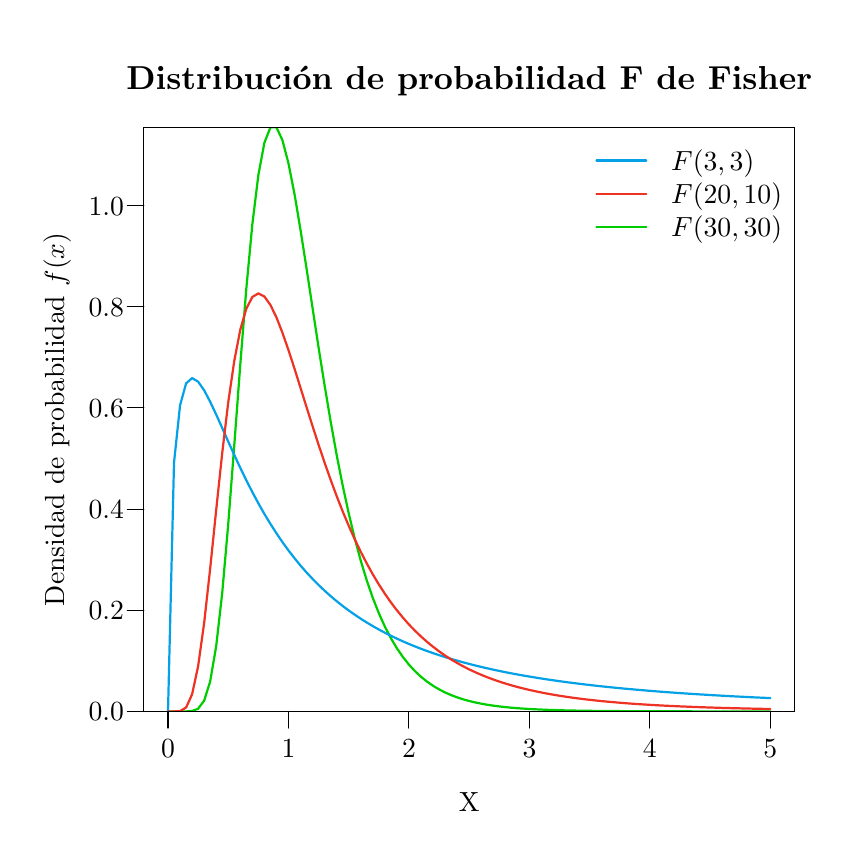
\begin{tikzpicture}[x=1pt,y=1pt]
\definecolor{fillColor}{RGB}{255,255,255}
\path[use as bounding box,fill=fillColor,fill opacity=0.00] (0,0) rectangle (289.08,289.08);
\begin{scope}
\path[clip] ( 42.00, 42.00) rectangle (277.08,253.08);
\definecolor{drawColor}{RGB}{0,205,0}

\path[draw=drawColor,line width= 0.8pt,line join=round,line cap=round] ( 50.71, 42.00) --
	( 52.88, 42.00) --
	( 55.06, 42.00) --
	( 57.24, 42.01) --
	( 59.41, 42.15) --
	( 61.59, 42.98) --
	( 63.77, 45.88) --
	( 65.94, 52.83) --
	( 68.12, 65.59) --
	( 70.30, 84.81) --
	( 72.47,109.69) --
	( 74.65,138.11) --
	( 76.83,167.37) --
	( 79.00,194.73) --
	( 81.18,218.02) --
	( 83.36,235.81) --
	( 85.53,247.47) --
	( 87.71,253.04) --
	( 89.89,253.08) --
	( 92.06,248.42) --
	( 94.24,240.04) --
	( 96.42,228.94) --
	( 98.59,216.01) --
	(100.77,202.06) --
	(102.95,187.72) --
	(105.12,173.50) --
	(107.30,159.77) --
	(109.48,146.78) --
	(111.65,134.71) --
	(113.83,123.63) --
	(116.01,113.57) --
	(118.18,104.53) --
	(120.36, 96.47) --
	(122.54, 89.32) --
	(124.71, 83.02) --
	(126.89, 77.50) --
	(129.07, 72.67) --
	(131.24, 68.47) --
	(133.42, 64.82) --
	(135.60, 61.66) --
	(137.77, 58.92) --
	(139.95, 56.56) --
	(142.13, 54.53) --
	(144.30, 52.78) --
	(146.48, 51.27) --
	(148.66, 49.97) --
	(150.83, 48.86) --
	(153.01, 47.91) --
	(155.19, 47.08) --
	(157.36, 46.38) --
	(159.54, 45.77) --
	(161.72, 45.25) --
	(163.89, 44.81) --
	(166.07, 44.42) --
	(168.25, 44.09) --
	(170.42, 43.81) --
	(172.60, 43.56) --
	(174.78, 43.35) --
	(176.95, 43.17) --
	(179.13, 43.02) --
	(181.31, 42.88) --
	(183.48, 42.77) --
	(185.66, 42.67) --
	(187.84, 42.58) --
	(190.01, 42.50) --
	(192.19, 42.44) --
	(194.37, 42.38) --
	(196.54, 42.33) --
	(198.72, 42.29) --
	(200.90, 42.25) --
	(203.07, 42.22) --
	(205.25, 42.20) --
	(207.43, 42.17) --
	(209.60, 42.15) --
	(211.78, 42.13) --
	(213.96, 42.12) --
	(216.13, 42.10) --
	(218.31, 42.09) --
	(220.49, 42.08) --
	(222.66, 42.07) --
	(224.84, 42.06) --
	(227.02, 42.05) --
	(229.19, 42.05) --
	(231.37, 42.04) --
	(233.55, 42.04) --
	(235.72, 42.03) --
	(237.90, 42.03) --
	(240.08, 42.03) --
	(242.25, 42.02) --
	(244.43, 42.02) --
	(246.61, 42.02) --
	(248.78, 42.02) --
	(250.96, 42.01) --
	(253.14, 42.01) --
	(255.31, 42.01) --
	(257.49, 42.01) --
	(259.67, 42.01) --
	(261.84, 42.01) --
	(264.02, 42.01) --
	(266.20, 42.01) --
	(268.37, 42.01);
\end{scope}
\begin{scope}
\path[clip] (  0.00,  0.00) rectangle (289.08,289.08);
\definecolor{drawColor}{RGB}{0,0,0}

\path[draw=drawColor,line width= 0.4pt,line join=round,line cap=round] ( 50.71, 42.00) -- (268.37, 42.00);

\path[draw=drawColor,line width= 0.4pt,line join=round,line cap=round] ( 50.71, 42.00) -- ( 50.71, 36.00);

\path[draw=drawColor,line width= 0.4pt,line join=round,line cap=round] ( 94.24, 42.00) -- ( 94.24, 36.00);

\path[draw=drawColor,line width= 0.4pt,line join=round,line cap=round] (137.77, 42.00) -- (137.77, 36.00);

\path[draw=drawColor,line width= 0.4pt,line join=round,line cap=round] (181.31, 42.00) -- (181.31, 36.00);

\path[draw=drawColor,line width= 0.4pt,line join=round,line cap=round] (224.84, 42.00) -- (224.84, 36.00);

\path[draw=drawColor,line width= 0.4pt,line join=round,line cap=round] (268.37, 42.00) -- (268.37, 36.00);

\node[text=drawColor,anchor=base,inner sep=0pt, outer sep=0pt, scale=  1.00] at ( 50.71, 25.20) {0};

\node[text=drawColor,anchor=base,inner sep=0pt, outer sep=0pt, scale=  1.00] at ( 94.24, 25.20) {1};

\node[text=drawColor,anchor=base,inner sep=0pt, outer sep=0pt, scale=  1.00] at (137.77, 25.20) {2};

\node[text=drawColor,anchor=base,inner sep=0pt, outer sep=0pt, scale=  1.00] at (181.31, 25.20) {3};

\node[text=drawColor,anchor=base,inner sep=0pt, outer sep=0pt, scale=  1.00] at (224.84, 25.20) {4};

\node[text=drawColor,anchor=base,inner sep=0pt, outer sep=0pt, scale=  1.00] at (268.37, 25.20) {5};

\path[draw=drawColor,line width= 0.4pt,line join=round,line cap=round] ( 42.00, 42.00) -- ( 42.00,224.78);

\path[draw=drawColor,line width= 0.4pt,line join=round,line cap=round] ( 42.00, 42.00) -- ( 36.00, 42.00);

\path[draw=drawColor,line width= 0.4pt,line join=round,line cap=round] ( 42.00, 78.56) -- ( 36.00, 78.56);

\path[draw=drawColor,line width= 0.4pt,line join=round,line cap=round] ( 42.00,115.11) -- ( 36.00,115.11);

\path[draw=drawColor,line width= 0.4pt,line join=round,line cap=round] ( 42.00,151.67) -- ( 36.00,151.67);

\path[draw=drawColor,line width= 0.4pt,line join=round,line cap=round] ( 42.00,188.23) -- ( 36.00,188.23);

\path[draw=drawColor,line width= 0.4pt,line join=round,line cap=round] ( 42.00,224.78) -- ( 36.00,224.78);

\node[text=drawColor,anchor=base east,inner sep=0pt, outer sep=0pt, scale=  1.00] at ( 34.80, 38.56) {0.0};

\node[text=drawColor,anchor=base east,inner sep=0pt, outer sep=0pt, scale=  1.00] at ( 34.80, 75.11) {0.2};

\node[text=drawColor,anchor=base east,inner sep=0pt, outer sep=0pt, scale=  1.00] at ( 34.80,111.67) {0.4};

\node[text=drawColor,anchor=base east,inner sep=0pt, outer sep=0pt, scale=  1.00] at ( 34.80,148.23) {0.6};

\node[text=drawColor,anchor=base east,inner sep=0pt, outer sep=0pt, scale=  1.00] at ( 34.80,184.78) {0.8};

\node[text=drawColor,anchor=base east,inner sep=0pt, outer sep=0pt, scale=  1.00] at ( 34.80,221.34) {1.0};

\path[draw=drawColor,line width= 0.4pt,line join=round,line cap=round] ( 42.00, 42.00) --
	(277.08, 42.00) --
	(277.08,253.08) --
	( 42.00,253.08) --
	( 42.00, 42.00);
\end{scope}
\begin{scope}
\path[clip] (  0.00,  0.00) rectangle (289.08,289.08);
\definecolor{drawColor}{RGB}{0,0,0}

\node[text=drawColor,anchor=base,inner sep=0pt, outer sep=0pt, scale=  1.20] at (159.54,266.89) {\bfseries Distribución de probabilidad F de Fisher};

\node[text=drawColor,anchor=base,inner sep=0pt, outer sep=0pt, scale=  1.00] at (159.54,  6.00) {X};

\node[text=drawColor,rotate= 90.00,anchor=base,inner sep=0pt, outer sep=0pt, scale=  1.00] at ( 13.20,147.54) {Densidad de probabilidad $f(x)$};
\end{scope}
\begin{scope}
\path[clip] ( 42.00, 42.00) rectangle (277.08,253.08);
\definecolor{drawColor}{RGB}{5,161,230}

\path[draw=drawColor,line width= 0.8pt,line join=round,line cap=round] ( 50.71, 42.00) --
	( 52.88,131.91) --
	( 55.06,152.59) --
	( 57.24,160.53) --
	( 59.41,162.46) --
	( 61.59,161.16) --
	( 63.77,158.04) --
	( 65.94,153.92) --
	( 68.12,149.28) --
	( 70.30,144.42) --
	( 72.47,139.52) --
	( 74.65,134.70) --
	( 76.83,130.02) --
	( 79.00,125.54) --
	( 81.18,121.26) --
	( 83.36,117.21) --
	( 85.53,113.38) --
	( 87.71,109.78) --
	( 89.89,106.38) --
	( 92.06,103.18) --
	( 94.24,100.18) --
	( 96.42, 97.36) --
	( 98.59, 94.71) --
	(100.77, 92.22) --
	(102.95, 89.89) --
	(105.12, 87.69) --
	(107.30, 85.62) --
	(109.48, 83.67) --
	(111.65, 81.84) --
	(113.83, 80.11) --
	(116.01, 78.48) --
	(118.18, 76.95) --
	(120.36, 75.50) --
	(122.54, 74.13) --
	(124.71, 72.83) --
	(126.89, 71.61) --
	(129.07, 70.45) --
	(131.24, 69.35) --
	(133.42, 68.31) --
	(135.60, 67.32) --
	(137.77, 66.38) --
	(139.95, 65.49) --
	(142.13, 64.64) --
	(144.30, 63.84) --
	(146.48, 63.07) --
	(148.66, 62.34) --
	(150.83, 61.64) --
	(153.01, 60.98) --
	(155.19, 60.35) --
	(157.36, 59.74) --
	(159.54, 59.17) --
	(161.72, 58.61) --
	(163.89, 58.09) --
	(166.07, 57.58) --
	(168.25, 57.10) --
	(170.42, 56.64) --
	(172.60, 56.19) --
	(174.78, 55.77) --
	(176.95, 55.36) --
	(179.13, 54.97) --
	(181.31, 54.60) --
	(183.48, 54.24) --
	(185.66, 53.89) --
	(187.84, 53.56) --
	(190.01, 53.24) --
	(192.19, 52.93) --
	(194.37, 52.63) --
	(196.54, 52.35) --
	(198.72, 52.08) --
	(200.90, 51.81) --
	(203.07, 51.56) --
	(205.25, 51.31) --
	(207.43, 51.07) --
	(209.60, 50.84) --
	(211.78, 50.62) --
	(213.96, 50.41) --
	(216.13, 50.20) --
	(218.31, 50.01) --
	(220.49, 49.81) --
	(222.66, 49.63) --
	(224.84, 49.45) --
	(227.02, 49.27) --
	(229.19, 49.10) --
	(231.37, 48.94) --
	(233.55, 48.78) --
	(235.72, 48.63) --
	(237.90, 48.48) --
	(240.08, 48.34) --
	(242.25, 48.20) --
	(244.43, 48.07) --
	(246.61, 47.93) --
	(248.78, 47.81) --
	(250.96, 47.68) --
	(253.14, 47.56) --
	(255.31, 47.45) --
	(257.49, 47.34) --
	(259.67, 47.23) --
	(261.84, 47.12) --
	(264.02, 47.02) --
	(266.20, 46.92) --
	(268.37, 46.82);
\definecolor{drawColor}{RGB}{238,50,36}

\path[draw=drawColor,line width= 0.8pt,line join=round,line cap=round] ( 50.71, 42.00) --
	( 52.88, 42.00) --
	( 55.06, 42.12) --
	( 57.24, 43.41) --
	( 59.41, 48.17) --
	( 61.59, 58.32) --
	( 63.77, 73.99) --
	( 65.94, 93.59) --
	( 68.12,114.80) --
	( 70.30,135.39) --
	( 72.47,153.67) --
	( 74.65,168.66) --
	( 76.83,179.94) --
	( 79.00,187.54) --
	( 81.18,191.76) --
	( 83.36,193.05) --
	( 85.53,191.93) --
	( 87.71,188.89) --
	( 89.89,184.39) --
	( 92.06,178.84) --
	( 94.24,172.57) --
	( 96.42,165.87) --
	( 98.59,158.94) --
	(100.77,151.96) --
	(102.95,145.07) --
	(105.12,138.35) --
	(107.30,131.87) --
	(109.48,125.69) --
	(111.65,119.82) --
	(113.83,114.28) --
	(116.01,109.08) --
	(118.18,104.22) --
	(120.36, 99.68) --
	(122.54, 95.46) --
	(124.71, 91.54) --
	(126.89, 87.90) --
	(129.07, 84.54) --
	(131.24, 81.42) --
	(133.42, 78.55) --
	(135.60, 75.89) --
	(137.77, 73.43) --
	(139.95, 71.17) --
	(142.13, 69.08) --
	(144.30, 67.15) --
	(146.48, 65.37) --
	(148.66, 63.72) --
	(150.83, 62.20) --
	(153.01, 60.80) --
	(155.19, 59.50) --
	(157.36, 58.31) --
	(159.54, 57.20) --
	(161.72, 56.18) --
	(163.89, 55.23) --
	(166.07, 54.35) --
	(168.25, 53.54) --
	(170.42, 52.79) --
	(172.60, 52.09) --
	(174.78, 51.44) --
	(176.95, 50.84) --
	(179.13, 50.29) --
	(181.31, 49.77) --
	(183.48, 49.29) --
	(185.66, 48.84) --
	(187.84, 48.42) --
	(190.01, 48.03) --
	(192.19, 47.67) --
	(194.37, 47.33) --
	(196.54, 47.02) --
	(198.72, 46.73) --
	(200.90, 46.45) --
	(203.07, 46.20) --
	(205.25, 45.96) --
	(207.43, 45.73) --
	(209.60, 45.52) --
	(211.78, 45.33) --
	(213.96, 45.15) --
	(216.13, 44.97) --
	(218.31, 44.81) --
	(220.49, 44.66) --
	(222.66, 44.52) --
	(224.84, 44.39) --
	(227.02, 44.26) --
	(229.19, 44.14) --
	(231.37, 44.03) --
	(233.55, 43.93) --
	(235.72, 43.83) --
	(237.90, 43.74) --
	(240.08, 43.65) --
	(242.25, 43.57) --
	(244.43, 43.49) --
	(246.61, 43.42) --
	(248.78, 43.35) --
	(250.96, 43.28) --
	(253.14, 43.22) --
	(255.31, 43.16) --
	(257.49, 43.11) --
	(259.67, 43.06) --
	(261.84, 43.01) --
	(264.02, 42.96) --
	(266.20, 42.92) --
	(268.37, 42.88);
\definecolor{drawColor}{RGB}{5,161,230}

\path[draw=drawColor,line width= 0.8pt,line join=round,line cap=round] (205.54,241.08) -- (223.54,241.08);
\definecolor{drawColor}{RGB}{238,50,36}

\path[draw=drawColor,line width= 0.8pt,line join=round,line cap=round] (205.54,229.08) -- (223.54,229.08);
\definecolor{drawColor}{RGB}{0,205,0}

\path[draw=drawColor,line width= 0.8pt,line join=round,line cap=round] (205.54,217.08) -- (223.54,217.08);
\definecolor{drawColor}{RGB}{0,0,0}

\node[text=drawColor,anchor=base west,inner sep=0pt, outer sep=0pt, scale=  1.00] at (232.54,237.64) {$F(3,3)$};

\node[text=drawColor,anchor=base west,inner sep=0pt, outer sep=0pt, scale=  1.00] at (232.54,225.64) {$F(20,10)$};

\node[text=drawColor,anchor=base west,inner sep=0pt, outer sep=0pt, scale=  1.00] at (232.54,213.64) {$F(30,30)$};
\end{scope}
\begin{scope}
\path[clip] (  0.00,  0.00) rectangle (289.08,289.08);
\definecolor{drawColor}{RGB}{0,0,0}

\path[draw=drawColor,line width= 0.4pt,line join=round,line cap=round] ( 42.00, 42.00) --
	(277.08, 42.00) --
	(277.08,253.08) --
	( 42.00,253.08) --
	( 42.00, 42.00);
\end{scope}
\end{tikzpicture}
}}
	\mode<presentation>{\resizebox{0.6\textwidth}{!}{% Created by tikzDevice version 0.10.1 on 2016-05-08 18:26:22
% !TEX encoding = UTF-8 Unicode
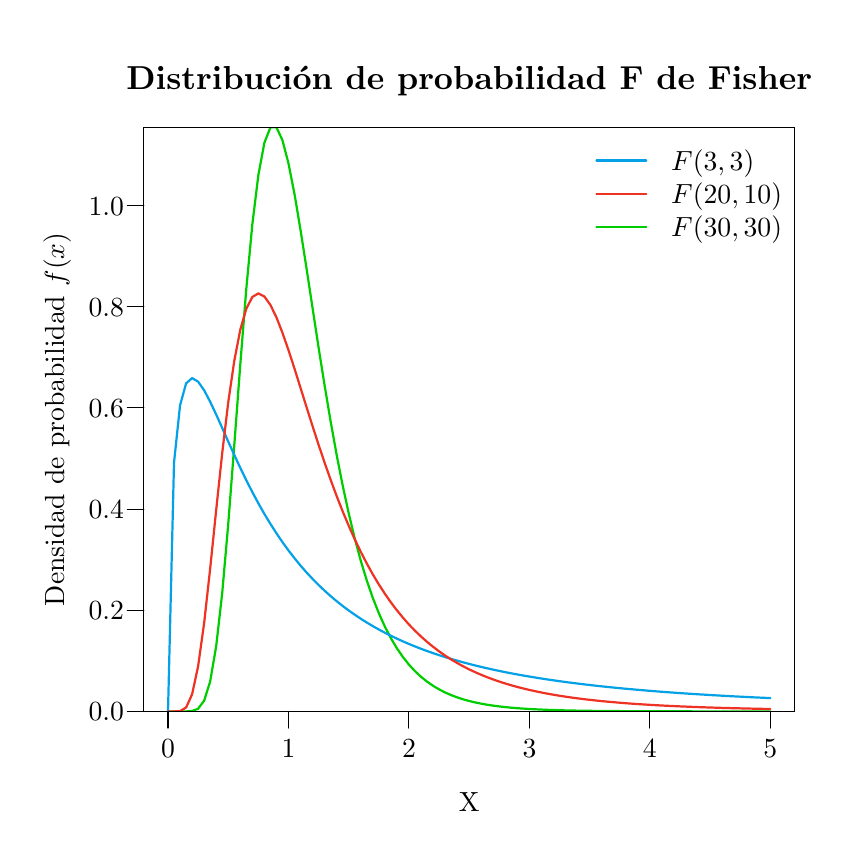
\begin{tikzpicture}[x=1pt,y=1pt]
\definecolor{fillColor}{RGB}{255,255,255}
\path[use as bounding box,fill=fillColor,fill opacity=0.00] (0,0) rectangle (289.08,289.08);
\begin{scope}
\path[clip] ( 42.00, 42.00) rectangle (277.08,253.08);
\definecolor{drawColor}{RGB}{0,205,0}

\path[draw=drawColor,line width= 0.8pt,line join=round,line cap=round] ( 50.71, 42.00) --
	( 52.88, 42.00) --
	( 55.06, 42.00) --
	( 57.24, 42.01) --
	( 59.41, 42.15) --
	( 61.59, 42.98) --
	( 63.77, 45.88) --
	( 65.94, 52.83) --
	( 68.12, 65.59) --
	( 70.30, 84.81) --
	( 72.47,109.69) --
	( 74.65,138.11) --
	( 76.83,167.37) --
	( 79.00,194.73) --
	( 81.18,218.02) --
	( 83.36,235.81) --
	( 85.53,247.47) --
	( 87.71,253.04) --
	( 89.89,253.08) --
	( 92.06,248.42) --
	( 94.24,240.04) --
	( 96.42,228.94) --
	( 98.59,216.01) --
	(100.77,202.06) --
	(102.95,187.72) --
	(105.12,173.50) --
	(107.30,159.77) --
	(109.48,146.78) --
	(111.65,134.71) --
	(113.83,123.63) --
	(116.01,113.57) --
	(118.18,104.53) --
	(120.36, 96.47) --
	(122.54, 89.32) --
	(124.71, 83.02) --
	(126.89, 77.50) --
	(129.07, 72.67) --
	(131.24, 68.47) --
	(133.42, 64.82) --
	(135.60, 61.66) --
	(137.77, 58.92) --
	(139.95, 56.56) --
	(142.13, 54.53) --
	(144.30, 52.78) --
	(146.48, 51.27) --
	(148.66, 49.97) --
	(150.83, 48.86) --
	(153.01, 47.91) --
	(155.19, 47.08) --
	(157.36, 46.38) --
	(159.54, 45.77) --
	(161.72, 45.25) --
	(163.89, 44.81) --
	(166.07, 44.42) --
	(168.25, 44.09) --
	(170.42, 43.81) --
	(172.60, 43.56) --
	(174.78, 43.35) --
	(176.95, 43.17) --
	(179.13, 43.02) --
	(181.31, 42.88) --
	(183.48, 42.77) --
	(185.66, 42.67) --
	(187.84, 42.58) --
	(190.01, 42.50) --
	(192.19, 42.44) --
	(194.37, 42.38) --
	(196.54, 42.33) --
	(198.72, 42.29) --
	(200.90, 42.25) --
	(203.07, 42.22) --
	(205.25, 42.20) --
	(207.43, 42.17) --
	(209.60, 42.15) --
	(211.78, 42.13) --
	(213.96, 42.12) --
	(216.13, 42.10) --
	(218.31, 42.09) --
	(220.49, 42.08) --
	(222.66, 42.07) --
	(224.84, 42.06) --
	(227.02, 42.05) --
	(229.19, 42.05) --
	(231.37, 42.04) --
	(233.55, 42.04) --
	(235.72, 42.03) --
	(237.90, 42.03) --
	(240.08, 42.03) --
	(242.25, 42.02) --
	(244.43, 42.02) --
	(246.61, 42.02) --
	(248.78, 42.02) --
	(250.96, 42.01) --
	(253.14, 42.01) --
	(255.31, 42.01) --
	(257.49, 42.01) --
	(259.67, 42.01) --
	(261.84, 42.01) --
	(264.02, 42.01) --
	(266.20, 42.01) --
	(268.37, 42.01);
\end{scope}
\begin{scope}
\path[clip] (  0.00,  0.00) rectangle (289.08,289.08);
\definecolor{drawColor}{RGB}{0,0,0}

\path[draw=drawColor,line width= 0.4pt,line join=round,line cap=round] ( 50.71, 42.00) -- (268.37, 42.00);

\path[draw=drawColor,line width= 0.4pt,line join=round,line cap=round] ( 50.71, 42.00) -- ( 50.71, 36.00);

\path[draw=drawColor,line width= 0.4pt,line join=round,line cap=round] ( 94.24, 42.00) -- ( 94.24, 36.00);

\path[draw=drawColor,line width= 0.4pt,line join=round,line cap=round] (137.77, 42.00) -- (137.77, 36.00);

\path[draw=drawColor,line width= 0.4pt,line join=round,line cap=round] (181.31, 42.00) -- (181.31, 36.00);

\path[draw=drawColor,line width= 0.4pt,line join=round,line cap=round] (224.84, 42.00) -- (224.84, 36.00);

\path[draw=drawColor,line width= 0.4pt,line join=round,line cap=round] (268.37, 42.00) -- (268.37, 36.00);

\node[text=drawColor,anchor=base,inner sep=0pt, outer sep=0pt, scale=  1.00] at ( 50.71, 25.20) {0};

\node[text=drawColor,anchor=base,inner sep=0pt, outer sep=0pt, scale=  1.00] at ( 94.24, 25.20) {1};

\node[text=drawColor,anchor=base,inner sep=0pt, outer sep=0pt, scale=  1.00] at (137.77, 25.20) {2};

\node[text=drawColor,anchor=base,inner sep=0pt, outer sep=0pt, scale=  1.00] at (181.31, 25.20) {3};

\node[text=drawColor,anchor=base,inner sep=0pt, outer sep=0pt, scale=  1.00] at (224.84, 25.20) {4};

\node[text=drawColor,anchor=base,inner sep=0pt, outer sep=0pt, scale=  1.00] at (268.37, 25.20) {5};

\path[draw=drawColor,line width= 0.4pt,line join=round,line cap=round] ( 42.00, 42.00) -- ( 42.00,224.78);

\path[draw=drawColor,line width= 0.4pt,line join=round,line cap=round] ( 42.00, 42.00) -- ( 36.00, 42.00);

\path[draw=drawColor,line width= 0.4pt,line join=round,line cap=round] ( 42.00, 78.56) -- ( 36.00, 78.56);

\path[draw=drawColor,line width= 0.4pt,line join=round,line cap=round] ( 42.00,115.11) -- ( 36.00,115.11);

\path[draw=drawColor,line width= 0.4pt,line join=round,line cap=round] ( 42.00,151.67) -- ( 36.00,151.67);

\path[draw=drawColor,line width= 0.4pt,line join=round,line cap=round] ( 42.00,188.23) -- ( 36.00,188.23);

\path[draw=drawColor,line width= 0.4pt,line join=round,line cap=round] ( 42.00,224.78) -- ( 36.00,224.78);

\node[text=drawColor,anchor=base east,inner sep=0pt, outer sep=0pt, scale=  1.00] at ( 34.80, 38.56) {0.0};

\node[text=drawColor,anchor=base east,inner sep=0pt, outer sep=0pt, scale=  1.00] at ( 34.80, 75.11) {0.2};

\node[text=drawColor,anchor=base east,inner sep=0pt, outer sep=0pt, scale=  1.00] at ( 34.80,111.67) {0.4};

\node[text=drawColor,anchor=base east,inner sep=0pt, outer sep=0pt, scale=  1.00] at ( 34.80,148.23) {0.6};

\node[text=drawColor,anchor=base east,inner sep=0pt, outer sep=0pt, scale=  1.00] at ( 34.80,184.78) {0.8};

\node[text=drawColor,anchor=base east,inner sep=0pt, outer sep=0pt, scale=  1.00] at ( 34.80,221.34) {1.0};

\path[draw=drawColor,line width= 0.4pt,line join=round,line cap=round] ( 42.00, 42.00) --
	(277.08, 42.00) --
	(277.08,253.08) --
	( 42.00,253.08) --
	( 42.00, 42.00);
\end{scope}
\begin{scope}
\path[clip] (  0.00,  0.00) rectangle (289.08,289.08);
\definecolor{drawColor}{RGB}{0,0,0}

\node[text=drawColor,anchor=base,inner sep=0pt, outer sep=0pt, scale=  1.20] at (159.54,266.89) {\bfseries Distribución de probabilidad F de Fisher};

\node[text=drawColor,anchor=base,inner sep=0pt, outer sep=0pt, scale=  1.00] at (159.54,  6.00) {X};

\node[text=drawColor,rotate= 90.00,anchor=base,inner sep=0pt, outer sep=0pt, scale=  1.00] at ( 13.20,147.54) {Densidad de probabilidad $f(x)$};
\end{scope}
\begin{scope}
\path[clip] ( 42.00, 42.00) rectangle (277.08,253.08);
\definecolor{drawColor}{RGB}{5,161,230}

\path[draw=drawColor,line width= 0.8pt,line join=round,line cap=round] ( 50.71, 42.00) --
	( 52.88,131.91) --
	( 55.06,152.59) --
	( 57.24,160.53) --
	( 59.41,162.46) --
	( 61.59,161.16) --
	( 63.77,158.04) --
	( 65.94,153.92) --
	( 68.12,149.28) --
	( 70.30,144.42) --
	( 72.47,139.52) --
	( 74.65,134.70) --
	( 76.83,130.02) --
	( 79.00,125.54) --
	( 81.18,121.26) --
	( 83.36,117.21) --
	( 85.53,113.38) --
	( 87.71,109.78) --
	( 89.89,106.38) --
	( 92.06,103.18) --
	( 94.24,100.18) --
	( 96.42, 97.36) --
	( 98.59, 94.71) --
	(100.77, 92.22) --
	(102.95, 89.89) --
	(105.12, 87.69) --
	(107.30, 85.62) --
	(109.48, 83.67) --
	(111.65, 81.84) --
	(113.83, 80.11) --
	(116.01, 78.48) --
	(118.18, 76.95) --
	(120.36, 75.50) --
	(122.54, 74.13) --
	(124.71, 72.83) --
	(126.89, 71.61) --
	(129.07, 70.45) --
	(131.24, 69.35) --
	(133.42, 68.31) --
	(135.60, 67.32) --
	(137.77, 66.38) --
	(139.95, 65.49) --
	(142.13, 64.64) --
	(144.30, 63.84) --
	(146.48, 63.07) --
	(148.66, 62.34) --
	(150.83, 61.64) --
	(153.01, 60.98) --
	(155.19, 60.35) --
	(157.36, 59.74) --
	(159.54, 59.17) --
	(161.72, 58.61) --
	(163.89, 58.09) --
	(166.07, 57.58) --
	(168.25, 57.10) --
	(170.42, 56.64) --
	(172.60, 56.19) --
	(174.78, 55.77) --
	(176.95, 55.36) --
	(179.13, 54.97) --
	(181.31, 54.60) --
	(183.48, 54.24) --
	(185.66, 53.89) --
	(187.84, 53.56) --
	(190.01, 53.24) --
	(192.19, 52.93) --
	(194.37, 52.63) --
	(196.54, 52.35) --
	(198.72, 52.08) --
	(200.90, 51.81) --
	(203.07, 51.56) --
	(205.25, 51.31) --
	(207.43, 51.07) --
	(209.60, 50.84) --
	(211.78, 50.62) --
	(213.96, 50.41) --
	(216.13, 50.20) --
	(218.31, 50.01) --
	(220.49, 49.81) --
	(222.66, 49.63) --
	(224.84, 49.45) --
	(227.02, 49.27) --
	(229.19, 49.10) --
	(231.37, 48.94) --
	(233.55, 48.78) --
	(235.72, 48.63) --
	(237.90, 48.48) --
	(240.08, 48.34) --
	(242.25, 48.20) --
	(244.43, 48.07) --
	(246.61, 47.93) --
	(248.78, 47.81) --
	(250.96, 47.68) --
	(253.14, 47.56) --
	(255.31, 47.45) --
	(257.49, 47.34) --
	(259.67, 47.23) --
	(261.84, 47.12) --
	(264.02, 47.02) --
	(266.20, 46.92) --
	(268.37, 46.82);
\definecolor{drawColor}{RGB}{238,50,36}

\path[draw=drawColor,line width= 0.8pt,line join=round,line cap=round] ( 50.71, 42.00) --
	( 52.88, 42.00) --
	( 55.06, 42.12) --
	( 57.24, 43.41) --
	( 59.41, 48.17) --
	( 61.59, 58.32) --
	( 63.77, 73.99) --
	( 65.94, 93.59) --
	( 68.12,114.80) --
	( 70.30,135.39) --
	( 72.47,153.67) --
	( 74.65,168.66) --
	( 76.83,179.94) --
	( 79.00,187.54) --
	( 81.18,191.76) --
	( 83.36,193.05) --
	( 85.53,191.93) --
	( 87.71,188.89) --
	( 89.89,184.39) --
	( 92.06,178.84) --
	( 94.24,172.57) --
	( 96.42,165.87) --
	( 98.59,158.94) --
	(100.77,151.96) --
	(102.95,145.07) --
	(105.12,138.35) --
	(107.30,131.87) --
	(109.48,125.69) --
	(111.65,119.82) --
	(113.83,114.28) --
	(116.01,109.08) --
	(118.18,104.22) --
	(120.36, 99.68) --
	(122.54, 95.46) --
	(124.71, 91.54) --
	(126.89, 87.90) --
	(129.07, 84.54) --
	(131.24, 81.42) --
	(133.42, 78.55) --
	(135.60, 75.89) --
	(137.77, 73.43) --
	(139.95, 71.17) --
	(142.13, 69.08) --
	(144.30, 67.15) --
	(146.48, 65.37) --
	(148.66, 63.72) --
	(150.83, 62.20) --
	(153.01, 60.80) --
	(155.19, 59.50) --
	(157.36, 58.31) --
	(159.54, 57.20) --
	(161.72, 56.18) --
	(163.89, 55.23) --
	(166.07, 54.35) --
	(168.25, 53.54) --
	(170.42, 52.79) --
	(172.60, 52.09) --
	(174.78, 51.44) --
	(176.95, 50.84) --
	(179.13, 50.29) --
	(181.31, 49.77) --
	(183.48, 49.29) --
	(185.66, 48.84) --
	(187.84, 48.42) --
	(190.01, 48.03) --
	(192.19, 47.67) --
	(194.37, 47.33) --
	(196.54, 47.02) --
	(198.72, 46.73) --
	(200.90, 46.45) --
	(203.07, 46.20) --
	(205.25, 45.96) --
	(207.43, 45.73) --
	(209.60, 45.52) --
	(211.78, 45.33) --
	(213.96, 45.15) --
	(216.13, 44.97) --
	(218.31, 44.81) --
	(220.49, 44.66) --
	(222.66, 44.52) --
	(224.84, 44.39) --
	(227.02, 44.26) --
	(229.19, 44.14) --
	(231.37, 44.03) --
	(233.55, 43.93) --
	(235.72, 43.83) --
	(237.90, 43.74) --
	(240.08, 43.65) --
	(242.25, 43.57) --
	(244.43, 43.49) --
	(246.61, 43.42) --
	(248.78, 43.35) --
	(250.96, 43.28) --
	(253.14, 43.22) --
	(255.31, 43.16) --
	(257.49, 43.11) --
	(259.67, 43.06) --
	(261.84, 43.01) --
	(264.02, 42.96) --
	(266.20, 42.92) --
	(268.37, 42.88);
\definecolor{drawColor}{RGB}{5,161,230}

\path[draw=drawColor,line width= 0.8pt,line join=round,line cap=round] (205.54,241.08) -- (223.54,241.08);
\definecolor{drawColor}{RGB}{238,50,36}

\path[draw=drawColor,line width= 0.8pt,line join=round,line cap=round] (205.54,229.08) -- (223.54,229.08);
\definecolor{drawColor}{RGB}{0,205,0}

\path[draw=drawColor,line width= 0.8pt,line join=round,line cap=round] (205.54,217.08) -- (223.54,217.08);
\definecolor{drawColor}{RGB}{0,0,0}

\node[text=drawColor,anchor=base west,inner sep=0pt, outer sep=0pt, scale=  1.00] at (232.54,237.64) {$F(3,3)$};

\node[text=drawColor,anchor=base west,inner sep=0pt, outer sep=0pt, scale=  1.00] at (232.54,225.64) {$F(20,10)$};

\node[text=drawColor,anchor=base west,inner sep=0pt, outer sep=0pt, scale=  1.00] at (232.54,213.64) {$F(30,30)$};
\end{scope}
\begin{scope}
\path[clip] (  0.00,  0.00) rectangle (289.08,289.08);
\definecolor{drawColor}{RGB}{0,0,0}

\path[draw=drawColor,line width= 0.4pt,line join=round,line cap=round] ( 42.00, 42.00) --
	(277.08, 42.00) --
	(277.08,253.08) --
	( 42.00,253.08) --
	( 42.00, 42.00);
\end{scope}
\end{tikzpicture}
}}
\end{center}

\note{
Aquí tenemos las gráfica de la función de densidad de varias distribuciones F de Fisher con distintos grados de libertad. Como se puede
apreciar, al igual que la distribución chi-cuadrado, no presenta valores negativos, y siempre es asimétrica hacia la izquierda.
}
\end{frame}


%---------------------------------------------------------------------slide----
\begin{frame}
\frametitle{Propiedades de la distribución F de Fisher-Snedecor $F(m,n)$}
\begin{itemize}
\item No está definida para valores negativos.
\item De la definición se deduce que
\[
F(m,n) =\frac{1}{F(n,m)}
\]
de manera que si llamamos $f(m,n)_p$ al valor que cumple que $P(F(m,n)≤f(m,n)_p)=p$, entonces se cumple
\[                                          
f(m,n)_p =\frac{1}{f(n,m)_{1−p}}
\]
Esto resulta muy útil para utilizar las tablas de su función de  distribución.
\end{itemize}

\note{
Algunas propiedades que tiene la distribución F de Fisher son:
\begin{itemize}
\item No está definida para valores negativos.
\item De la definición se deduce que
\[
F(m,n) =\frac{1}{F(n,m)}
\]
de manera que si llamamos $f(m,n)_p$ al valor que cumple que $P(F(m,n)≤f(m,n)_p)=p$, entonces se cumple
\[                                          
f(m,n)_p =\frac{1}{f(n,m)_{1−p}}
\]
Esto resulta muy útil para utilizar las tablas de su función de distribución.
\end{itemize}
}
\end{frame}
